% Options for packages loaded elsewhere
\PassOptionsToPackage{unicode}{hyperref}
\PassOptionsToPackage{hyphens}{url}
%
\documentclass[
]{article}
\title{Comparing human and model-based forecasts of COVID-19 in Germany and Poland}
\author{}
\date{\vspace{-2.5em}}

\usepackage{amsmath,amssymb}
\usepackage{lmodern}
\usepackage{iftex}
\ifPDFTeX
  \usepackage[T1]{fontenc}
  \usepackage[utf8]{inputenc}
  \usepackage{textcomp} % provide euro and other symbols
\else % if luatex or xetex
  \usepackage{unicode-math}
  \defaultfontfeatures{Scale=MatchLowercase}
  \defaultfontfeatures[\rmfamily]{Ligatures=TeX,Scale=1}
\fi
% Use upquote if available, for straight quotes in verbatim environments
\IfFileExists{upquote.sty}{\usepackage{upquote}}{}
\IfFileExists{microtype.sty}{% use microtype if available
  \usepackage[]{microtype}
  \UseMicrotypeSet[protrusion]{basicmath} % disable protrusion for tt fonts
}{}
\makeatletter
\@ifundefined{KOMAClassName}{% if non-KOMA class
  \IfFileExists{parskip.sty}{%
    \usepackage{parskip}
  }{% else
    \setlength{\parindent}{0pt}
    \setlength{\parskip}{6pt plus 2pt minus 1pt}}
}{% if KOMA class
  \KOMAoptions{parskip=half}}
\makeatother
\usepackage{xcolor}
\IfFileExists{xurl.sty}{\usepackage{xurl}}{} % add URL line breaks if available
\IfFileExists{bookmark.sty}{\usepackage{bookmark}}{\usepackage{hyperref}}
\hypersetup{
  pdftitle={Comparing human and model-based forecasts of COVID-19 in Germany and Poland},
  hidelinks,
  pdfcreator={LaTeX via pandoc}}
\urlstyle{same} % disable monospaced font for URLs
\usepackage[margin=1in]{geometry}
\usepackage{longtable,booktabs,array}
\usepackage{calc} % for calculating minipage widths
% Correct order of tables after \paragraph or \subparagraph
\usepackage{etoolbox}
\makeatletter
\patchcmd\longtable{\par}{\if@noskipsec\mbox{}\fi\par}{}{}
\makeatother
% Allow footnotes in longtable head/foot
\IfFileExists{footnotehyper.sty}{\usepackage{footnotehyper}}{\usepackage{footnote}}
\makesavenoteenv{longtable}
\usepackage{graphicx}
\makeatletter
\def\maxwidth{\ifdim\Gin@nat@width>\linewidth\linewidth\else\Gin@nat@width\fi}
\def\maxheight{\ifdim\Gin@nat@height>\textheight\textheight\else\Gin@nat@height\fi}
\makeatother
% Scale images if necessary, so that they will not overflow the page
% margins by default, and it is still possible to overwrite the defaults
% using explicit options in \includegraphics[width, height, ...]{}
\setkeys{Gin}{width=\maxwidth,height=\maxheight,keepaspectratio}
% Set default figure placement to htbp
\makeatletter
\def\fps@figure{htbp}
\makeatother
\setlength{\emergencystretch}{3em} % prevent overfull lines
\providecommand{\tightlist}{%
  \setlength{\itemsep}{0pt}\setlength{\parskip}{0pt}}
\setcounter{secnumdepth}{5}
\newlength{\cslhangindent}
\setlength{\cslhangindent}{1.5em}
\newlength{\csllabelwidth}
\setlength{\csllabelwidth}{3em}
\newlength{\cslentryspacingunit} % times entry-spacing
\setlength{\cslentryspacingunit}{\parskip}
\newenvironment{CSLReferences}[2] % #1 hanging-ident, #2 entry spacing
 {% don't indent paragraphs
  \setlength{\parindent}{0pt}
  % turn on hanging indent if param 1 is 1
  \ifodd #1
  \let\oldpar\par
  \def\par{\hangindent=\cslhangindent\oldpar}
  \fi
  % set entry spacing
  \setlength{\parskip}{#2\cslentryspacingunit}
 }%
 {}
\usepackage{calc}
\newcommand{\CSLBlock}[1]{#1\hfill\break}
\newcommand{\CSLLeftMargin}[1]{\parbox[t]{\csllabelwidth}{#1}}
\newcommand{\CSLRightInline}[1]{\parbox[t]{\linewidth - \csllabelwidth}{#1}\break}
\newcommand{\CSLIndent}[1]{\hspace{\cslhangindent}#1}
\usepackage{float}
\usepackage{booktabs}
\usepackage{longtable}
\usepackage{array}
\usepackage{multirow}
\usepackage{wrapfig}
\usepackage{colortbl}
\usepackage{pdflscape}
\usepackage{tabu}
\usepackage{threeparttable}
\usepackage{threeparttablex}
\usepackage[normalem]{ulem}
\usepackage{makecell}
\usepackage{xcolor}
\ifLuaTeX
  \usepackage{selnolig}  % disable illegal ligatures
\fi

\begin{document}
\maketitle

{
\setcounter{tocdepth}{2}
\tableofcontents
}
\emph{Anonymous Alpaca and many friends}

\hypertarget{abstract-max-200-words-no-subheadings}{%
\section{Abstract (max 200 words, no subheadings)}\label{abstract-max-200-words-no-subheadings}}

Model-based forecasts, which have played an important role in shaping public policy throughout the COVID-19 pandemic, represent an implicit combination of model assumptions and the researcher's subjective opinion. This work analyses and compares human opinion against model-derived insights to discern relative strengths and weaknesses of both approaches. We compared purely opinion-derived forecasts of cases and deaths from COVID-19 in Germany and Poland, elicited from researchers and volunteers, against predictions from two semi-mechanistic epidemiological models. We also compared these forecasts against an ensemble of model-based, but expert-tuned, forecasts, submitted to the German and Polish Forecast Hub by other research institutions. In addition, we examined the effects of our contributions to the performance of the Hub ensemble. We found aggregated crowd forecasts to outperform all other methods when predicting cases (Weighted Interval Score relative to the Hub ensemble: 0.89), but not when predicting deaths (rel. WIS 1.26). Crowd forecasts were noticeably more overconfident (55\% and 75\% coverage of the 90\% prediction intervals for cases and deaths, respectively) than model-based predictions. Performance of the semi-mechanistic models was good short-term, but deteriorated quickly over time when assumptions were no longer met.

\hypertarget{introduction}{%
\section{Introduction}\label{introduction}}

Infectious disease forecasting has a long tradition and has helped inform public health decisions about (among others) influenza (e.g. McGowan et al. 2019; Reich et al. 2019; Shaman and Karspeck 2012; Biggerstaff et al. 2016), dengue fever (e.g. Johansson et al. 2019; Yamana, Kandula, and Shaman 2016; Colón-González et al. 2021), ebola (e.g. Viboud et al. 2018; Funk et al. 2019), chikungunya (e.g. Del Valle et al. 2018; Farrow et al. 2017) and now COVID-19 (e.g. Funk et al. 2020; Cramer et al. 2020; Cramer et al. 2021; Bracher, Wolffram, et al. 2021; Hub 2021). The aggregation of forecasts of COVID-19 cases, hospitalisations or deaths from multiple teams has created opportunities to compare the predictive performance of different models. Yet it has been difficult to discern which factors lead to good COVID-19 forecasts. Answering this question is complicated by the varying and generally unobserved degree of manual expert intervention. Model-based forecasts usually represent an implicit combination of human judgement and model-derived insights, in the sense that forecasts have been generated with the help of epidemiological or statistical models, but throughout the process were manually changed and adjusted according to the researchers' judgement.

Previous work has examined human predictions in various contexts, such as geopolitics (Tetlock et al. 2014; Atanasov et al. 2016), meta-science (Hoogeveen, Sarafoglou, and Wagenmakers 2020; {``Replication {Markets} -- {Reliable} Research Replicates\ldots you Can Bet on It.''} n.d.), sports (Servan-Schreiber et al. 2004) and epidemiology Recchia, Freeman, and Spiegelhalter (2021). Several prediction platforms (Metaculus 2020; {``Hypermind \textbar{} {Supercollective} Intelligence for Decision Makers''} n.d.; {``{CSET Foretell}''} n.d.) and prediction markets ({``{PredictIt}''} n.d.) have been created to collate expert and non-expert predictions. However, with the notable exception of Farrow et al., these crowd forecasts were not designed to be evaluated alongside model-based forecasts and usually follow their own (often binary) formats. Farrow et al.~found that humans could outperform computer models at predicting the 2014/15 and 2015/16 flu season in the US, a setting where the disease was well known and information about previous seasons was available. They tended to do slightly worse at predicting the 2014/15 outbreak of chikungunya in the Americas, a disease previously largely unobserved and unknown there and then.

In this study, we attempt to further shed light on the role of human judgement and model-derived insight and analyse respective strengths and weaknesses. To allow for a direct comparison on an equal footing we employ a novel approach that elicits full probabilistic forecasts (Held, Meyer, and Bracher 2017) from participants, rather than constructing a predictive distribution from individual point predictions.

\hypertarget{methods}{%
\section{Methods}\label{methods}}

We created a crowd-sourced forecast (``crowd forecast''), elicited from participants through a web application (N. I. Bosse et al. 2020), as well as two semi-mechanistic models (``renewal model'' and ``convolution model'') informed by basic assumptions about COVID-19 epidemiology. Forecasts were created in real time over a period of 21 weeks from October 12th 2020 until March 1st 2021 and submitted to the German and Polish Forecast hub (Bracher, Wolffram, et al. 2021). All code and tools necessary to generate the forecasts and make a forecast submission are available in the \texttt{covid.german.forecasts} R package (N. Bosse et al. 2020). This repository also contains a record of all forecasts submitted to the German and Polish Forecast Hub. Forecasts were evaluated using a variety of scoring metrics and compared among each other and against an ensemble of all other models submitted to the Forecast Hub.

\hypertarget{forecast-targets-and-interaction-with-the-german-and-polish-forecast-hub}{%
\subsection{Forecast targets and interaction with the German and Polish Forecast Hub}\label{forecast-targets-and-interaction-with-the-german-and-polish-forecast-hub}}

The German and Polish Forecast Hub elicits predictions for various COVID-19 related forecast targets from different research institutions every week. Forecasts had to be made every Monday (with submissions allowed until Tuesday 3pm) using data available until Monday 11.59pm. We submitted forecasts for incident and cumulative weekly reported numbers of cases and deaths from COVID-19 on a national level in Germany and Poland over a one to four week forecast horizon. Weeks were defined as epiweeks starting on Sunday and ending on Saturday, meaning that forecast horizons were in fact 5, 12, 19 and 26 days. Submissions were required in a quantile-based format with 23 quantiles at levels 0.01, 0.025, 0.05, 0.10, 0.15, \ldots, 0.95, 0.975, 0.99. Forecasts submitted to the Forecast Hub were combined to different ensembles every week, with the median ensemble being the default ensemble shown on all official Forecast hub visualisations.

Data on daily reported test positive cases and deaths linked to COVID-19 were provided by the organisers of the German and Polish forecast hub. Until December 14th 2020 these data were sourced from the European Centre for Disease Control (ECDC) ({``Download Historical Data (to 14 {December} 2020) on the Daily Number of New Reported {COVID}-19 Cases and Deaths Worldwide''} 2020). After ECDC stopped publishing daily data, observations were sourced from the Robert Koch Institute (RKI) and the Polish Ministry of Health for the remainder of the submission period ({``{RKI} - {Coronavirus SARS}-{CoV}-2 - {Aktueller Lage}-/{Situationsbericht} Des {RKI} Zu {COVID}-19''} n.d.). These data are subject to reporting artefacts (such as a delayed case reporting in Poland on the 24th November ({``Rozbieżności w statystykach koronawirusa. 22 tys. przypadków będą doliczone do ogólnej liczby wyników''} 16:07:56+0100)), changes in reporting over time and variation in testing regimes (e.g.~in Germany from the 11th of November on (Ärzteblatt 2020)).

\hypertarget{crowd-forecasts}{%
\subsection{Crowd forecasts}\label{crowd-forecasts}}

Our crowd forecasts were created as an ensemble of forecasts made by individual participants every week through a web application (\url{https://cmmid-lshtm.shinyapps.io/crowd-forecast/}). Forecasts were allowed until 12pm on Tuesdays, but participants were asked to only use information available until Monday. The application was built using the shiny and golem R packages (Fay et al. 2021; Chang et al. 2021) and is available in the \texttt{crowdforecastr} R package (N. I. Bosse et al. 2020). To make a forecast in the application participants could select a predictive distribution, with the default being log-normal, and adjust the median and the width of the uncertainty by either interacting with a figure showing their forecast or providing numerical values. The baseline shown was a repetition of the last known observation with constant uncertainty around it computed as the standard deviation of the last four changes in log observed forecasts (i.e.~as \texttt{sd(c(log(value4)\ -\ log(value3),\ log(value3)\ -\ log(value2),\ ...))}).
Our interface also allowed participants to view the observed data, and their forecasts, on a logarithmic scale and presented additional contextual COVID-19 data sourced from ({``{COVID}-19 {Data Explorer}''} n.d.). These data included e.g.~notifications of both test positive COVID-19 cases and COVID-19 linked deaths and the number of COVID-19 tests conducted over time.

Forecasts were stored in a Google Sheet and downloaded, cleaned and processed every week for submission. If a forecaster had submitted multiple predictions for a single target, only the latest submission was kept. Information on the chosen distribution as well as the parameters for median and width were used to obtain the required set of 23 quantiles from that distribution. Forecasts from all forecasters were then aggregated using an unweighted quantile-wise mean. On a few occasions, individual forecasts were assessed as clearly erroneous by visual inspection and subsequently removed before aggregation.

Participants were recruited mostly within the Centre of Mathematical Modeling of Infectious Diseases at the London School of Hygiene \& Tropical Medicine, but participants were also invited personally or via social media to submit predictions. Depending on whether they had a background in either statistics, forecasting or epidemiology, participants were asked to self-identify as `experts' or `non-experts.'

\hypertarget{model-based-forecasts}{%
\subsection{Model-based forecasts}\label{model-based-forecasts}}

We used two models from the \texttt{EpiNow2} R package (version 1.3.3) as our model-based forecasts (Abbott, Hellewell, et al. 2020). The first of these models, here called ``renewal model,'' used the renewal equation (Fraser 2007) to predict reported cases and deaths. It estimated the effective reproduction number \(R_t\) (the average number of people each infected person is expected to infect in turn) and models future infections as a weighted sum of past infection multiplied by \(R_t\). \(R_t\) was assumed to stay constant beyond the forecast horizon, roughly corresponding to continuing the latest exponential trend in infections. On the 9th of November we altered the date when \(R_t\) was assumed to be constant from two weeks prior to the date of the forecast to the forecast date. Reported notifications were obtained by convolving predicted infections over data-based delay distributions (Abbott, Hellewell, et al. 2020; DOI n.d.; {``Evaluating the Use of the Reproduction Number as an Epidemiological Tool, Using Spatio-Temporal Trends of the {Covid}-19 Outbreak in {England} \textbar{} {medRxiv}''} n.d.) to model the time between infection and report date or death. The renewal model was used to predict cases as well as deaths with forecasts being generated for each target separately, meaning that \(R_t\) was forecast once from reported cases and once from reported deaths. Death forecasts from the renewal model were therefore not informed by past cases. One submission of the renewal model on December 28th 2020 was delayed and therefore not included in the official Forecast hub ensemble.

The second model (``convolution model'') was only used to forecast deaths and was added later, starting December 7th 2020 (with the first forecast from December 7th suffering from a software bug and therefore disregarded in all further analyses). The convolution model was submitted, but never included in the official Forecast hub ensemble due to concerns that it could be too similar to the renewal model. The convolution model predicted deaths as a fraction of infected people who would die with some delay, by using a convolution of reported cases with a distribution that described the delay from case report to death and a scaling factor (the case-fatality ratio). Both the renewal and the convolution model used daily observations and assumed a negative binomial observation model with a multiplicative day-of-the-week effect (Abbott, Hellewell, et al. 2020). Line list data used to inform the prior for the delay from symptom onset to test positive case report or death in the model-based forecasts was sourced from (Xu et al., n.d.) with data available up to the 1st of August. All model fitting was done using Markov-chain Monte Carlo (MCMC) in stan (Stan Development Team 2020) with each location and forecast target being fit separately. More details are available in the supplementary information.

\hypertarget{analysis}{%
\subsection{Analysis}\label{analysis}}

For the main analysis we focused on two week ahead predictions, as predictions beyond this horizon are often unreliable due to rapidly changing conditions (Bracher, Wolffram, et al. 2021). Forecasts for cases were scored using the full period from October 2020 until March 2021. To ensure comparability between models, all death forecasts were scored using only the period from December 14th on, where all models including the convolution model were available. To ensure robustness of our results we conducted a sensitivity analysis where all forecasts (including cases) were scored only over the later period where forecasts were available (see Section \ref{sensitivity-analysis} in the SI). Results remained broadly unchanged.

Forecasts were analysed using the following scoring metrics: The weighted interval score (WIS) (Bracher, Ray, et al. 2021), the absolute error, relative bias, and empirical coverage of the 50\% and 90\% prediction intervals. The WIS is a proper scoring rule (Gneiting and Raftery 2007) and can be understood as a generalisation of the absolute error to quantile-based forecasts. It can be decomposed into three separate penalties: forecast spread (i.e.~uncertainty of forecasts), over-prediction and under-prediction - lower values are always better. While the over- and under-prediction components of the WIS capture the amount of over-prediction and under-prediction in absolute terms, we also look at a relative tendency to make biased forecasts. The bias metric we use captures how much probability mass of the forecast was above or below the true value and therefore represents a general tendency to over- or under-predict in relative terms. It is bound between -1 (all quantiles of the predictive distribution are below the observed value) and 1 (all quantiles are above the observed value). Empirical coverage is the percentage of observed values that fall inside a given prediction interval (e.g.~how many observed values fall inside all 50\% prediction intervals). Scoring metrics are explained in more detail in Table \ref{tab:scoring-metrics} in the SI. All scores were calculated using the \texttt{scoringutils} R package (N. Bosse 2020).

At all stages of the evaluation our forecasts were compared to the median ensemble of all other models submitted to the German and Polish Forecast Hub (``Hub ensemble''). This ``Hub ensemble'' was retrospectively computed and excludes all our models. It therefore differs from the official Hub ensemble (here called ``hub-ensemble-realised'') which included crowd forecasts as well as renewal model forecasts.

The ensemble that we call ``Hub ensemble'' in this paper differs from the

in that we removed our forecasts to allow for a more straightforward comparison. To enhance interpretability of scores we mainly report WIS relative to the Hub ensemble in the main text, i.e.~we divided all scores by those achieved by the Hub ensemble on the same set of forecasts. In addition to comparing our forecasts against the hub ensemble excluding our models, we also assessed the impact of our forecasts on the performance of the forecasting hub by recalculating separate versions of the Hub ensemble with only some (or all) of our forecasts included.

Versions that included either all of our models (``hub-ensemble-with-all'') or only one of them (``hub-ensemble-with-X'') were computed retrospectively.

\hypertarget{results}{%
\section{Results}\label{results}}

\hypertarget{crowd-forecast-participation}{%
\subsection{Crowd forecast participation}\label{crowd-forecast-participation}}

A total number of 32 participants submitted forecasts, 17 of those self-identified as `expert.' The median number of forecasters for any given forecast target was 6, the minimum 2 and the maximum 10. The mean number of submissions from an individual forecaster was 4.7 but the median number was only one - most participants dropped out after their first submission. Only two participants submitted a forecast every single week, both of whom are authors on this study.

\begin{figure}[H]
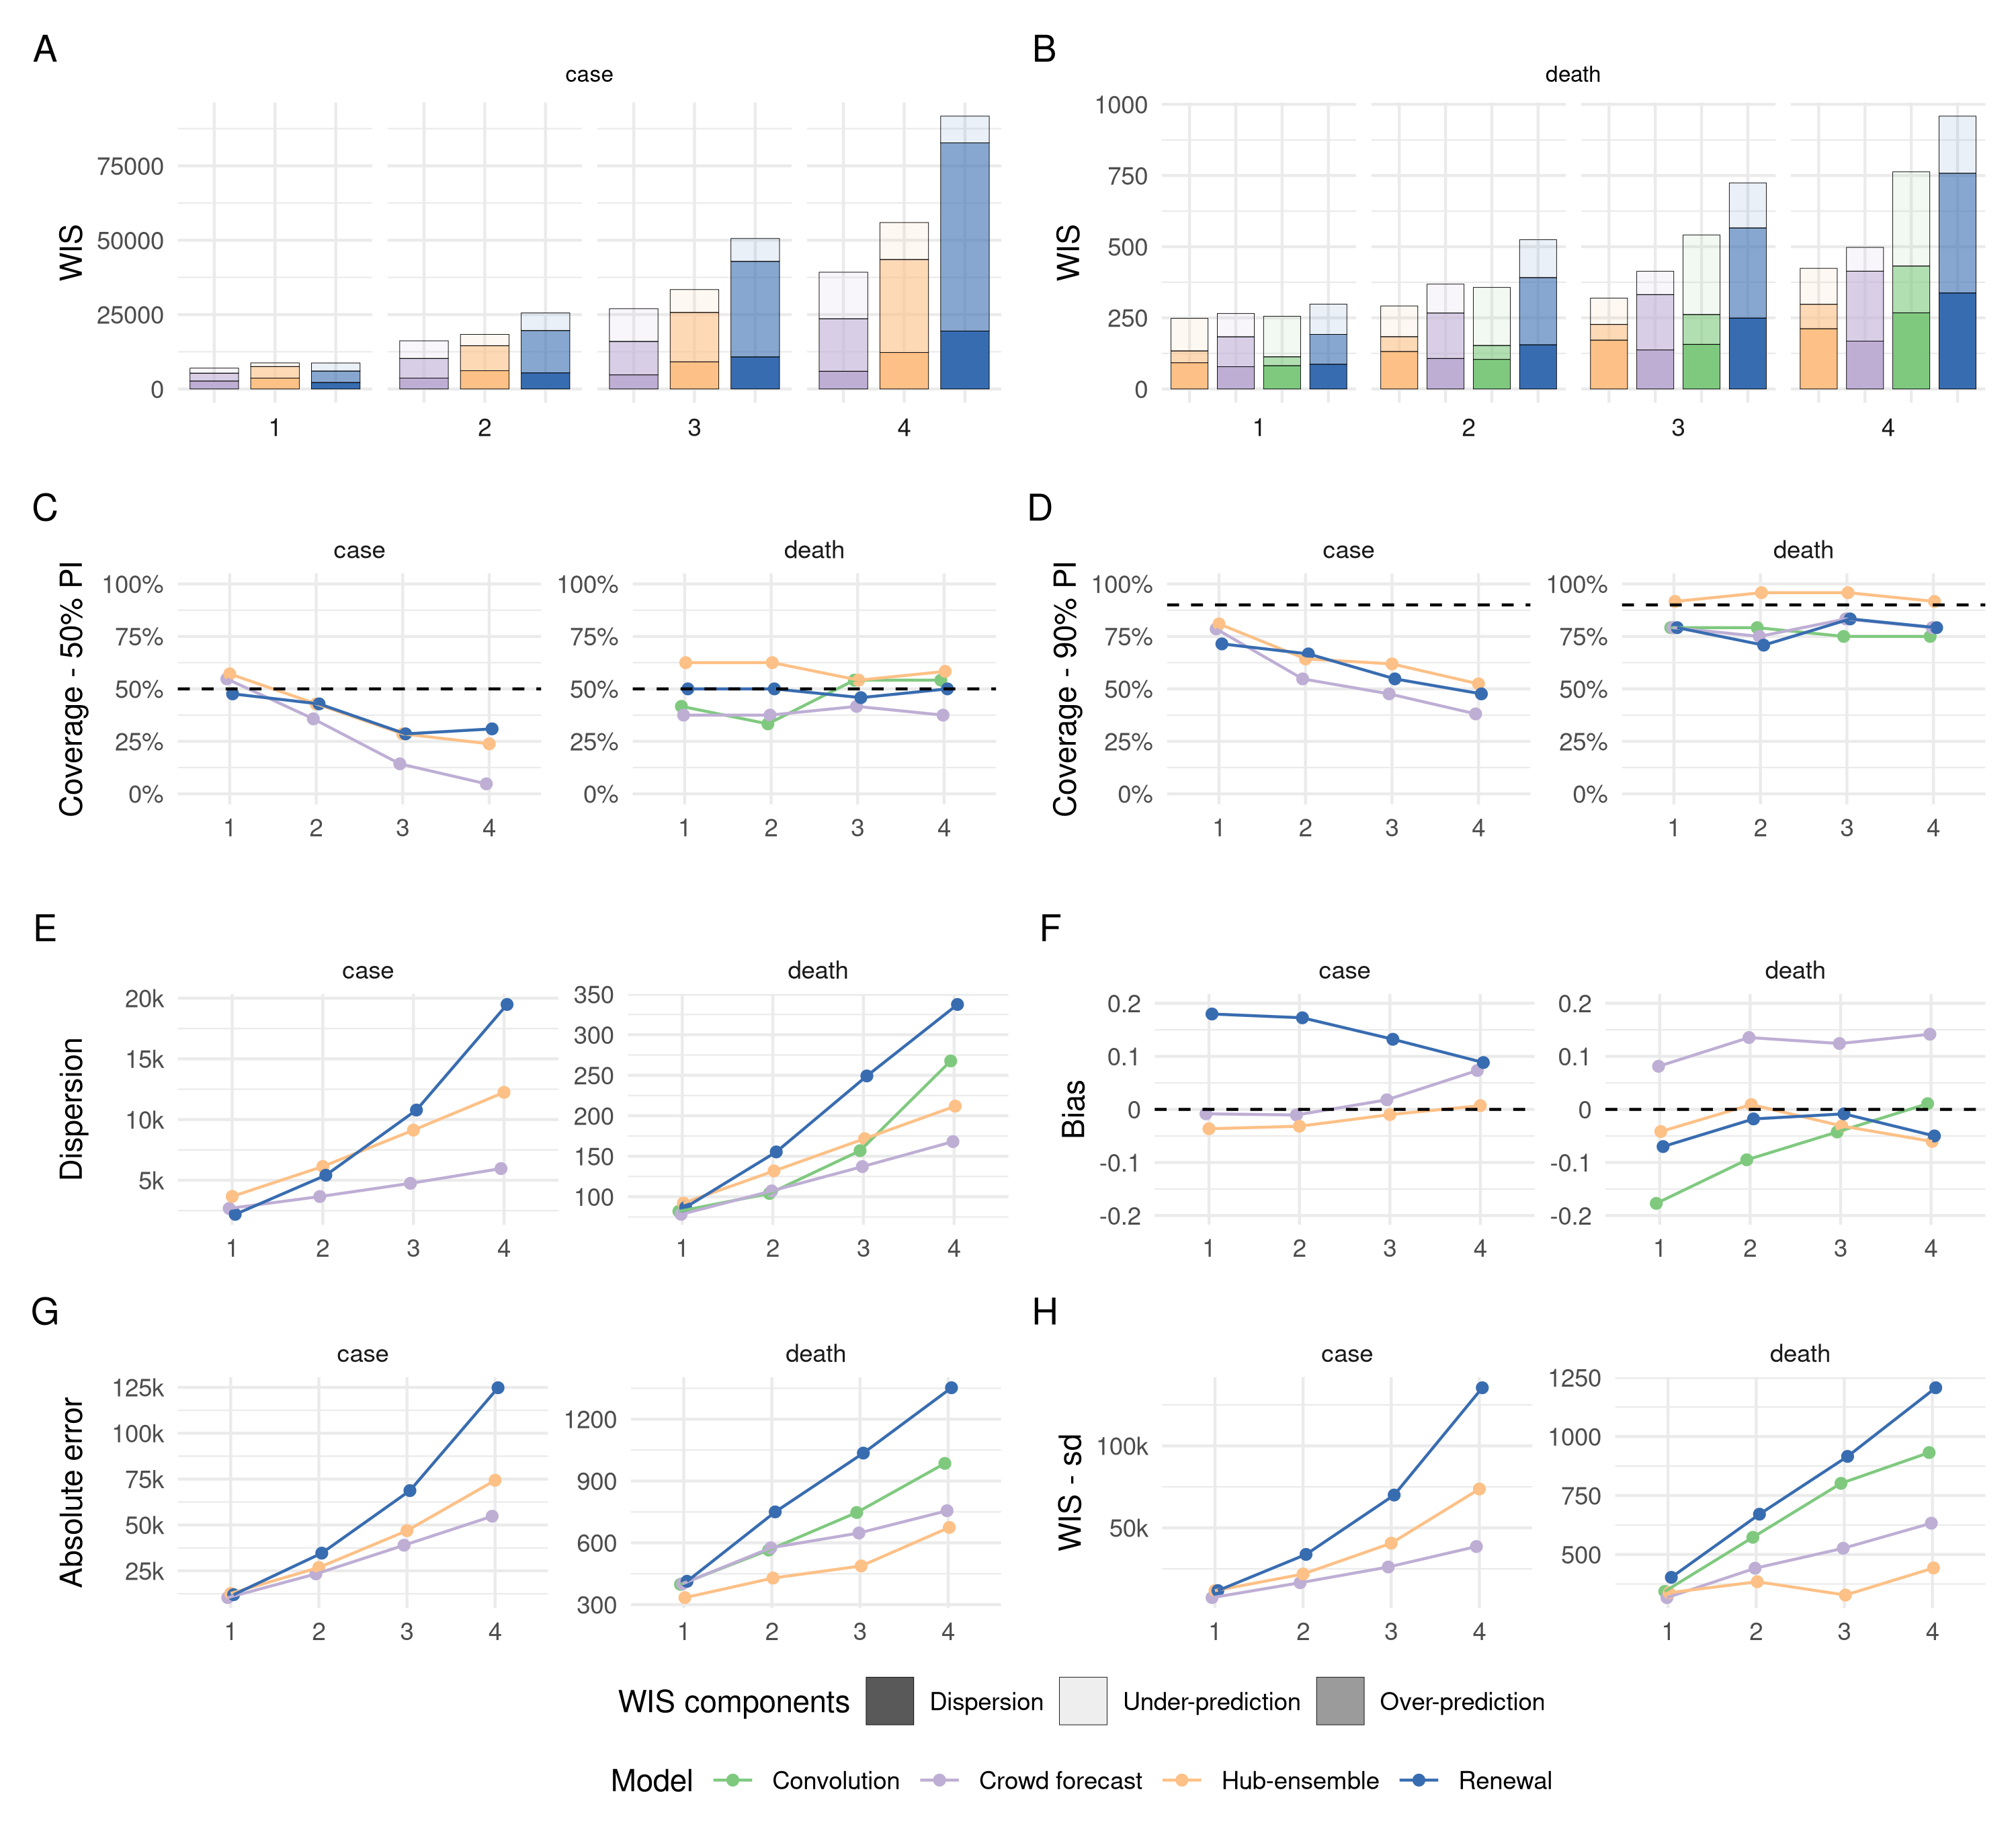
\includegraphics[width=1\linewidth,]{../analysis/plots/aggregate-performance-all-v4} \caption{Visualisation of aggregate performance metrics across forecast horizons. A, B: mean weighted interval score (WIS, lower indicates better performance) across horizons. WIS is decomposed into its components dispersion, over-prediction and under-prediction. C: Empirical coverage of the 50\% prediction intervals (50\% coverage is perfect). D: Empirical coverage of the 90\% prediction intervals. E: Dispersion (same as in panel A, B). Higher values mean greater dispersion of the forecast and imply ceteris paribus a worse score. F: Bias, i.e. general (relative) tendency to over- or underpredict. Values are between -1 (complete under-prediction) and 1 (complete over-prediction) and 0 ideally. G: Absolute error of the median forecast (lower is better). H. Standard deviation of all WIS values for different horizons}\label{fig:agg-performance-all}
\end{figure}

\begin{figure}[H]
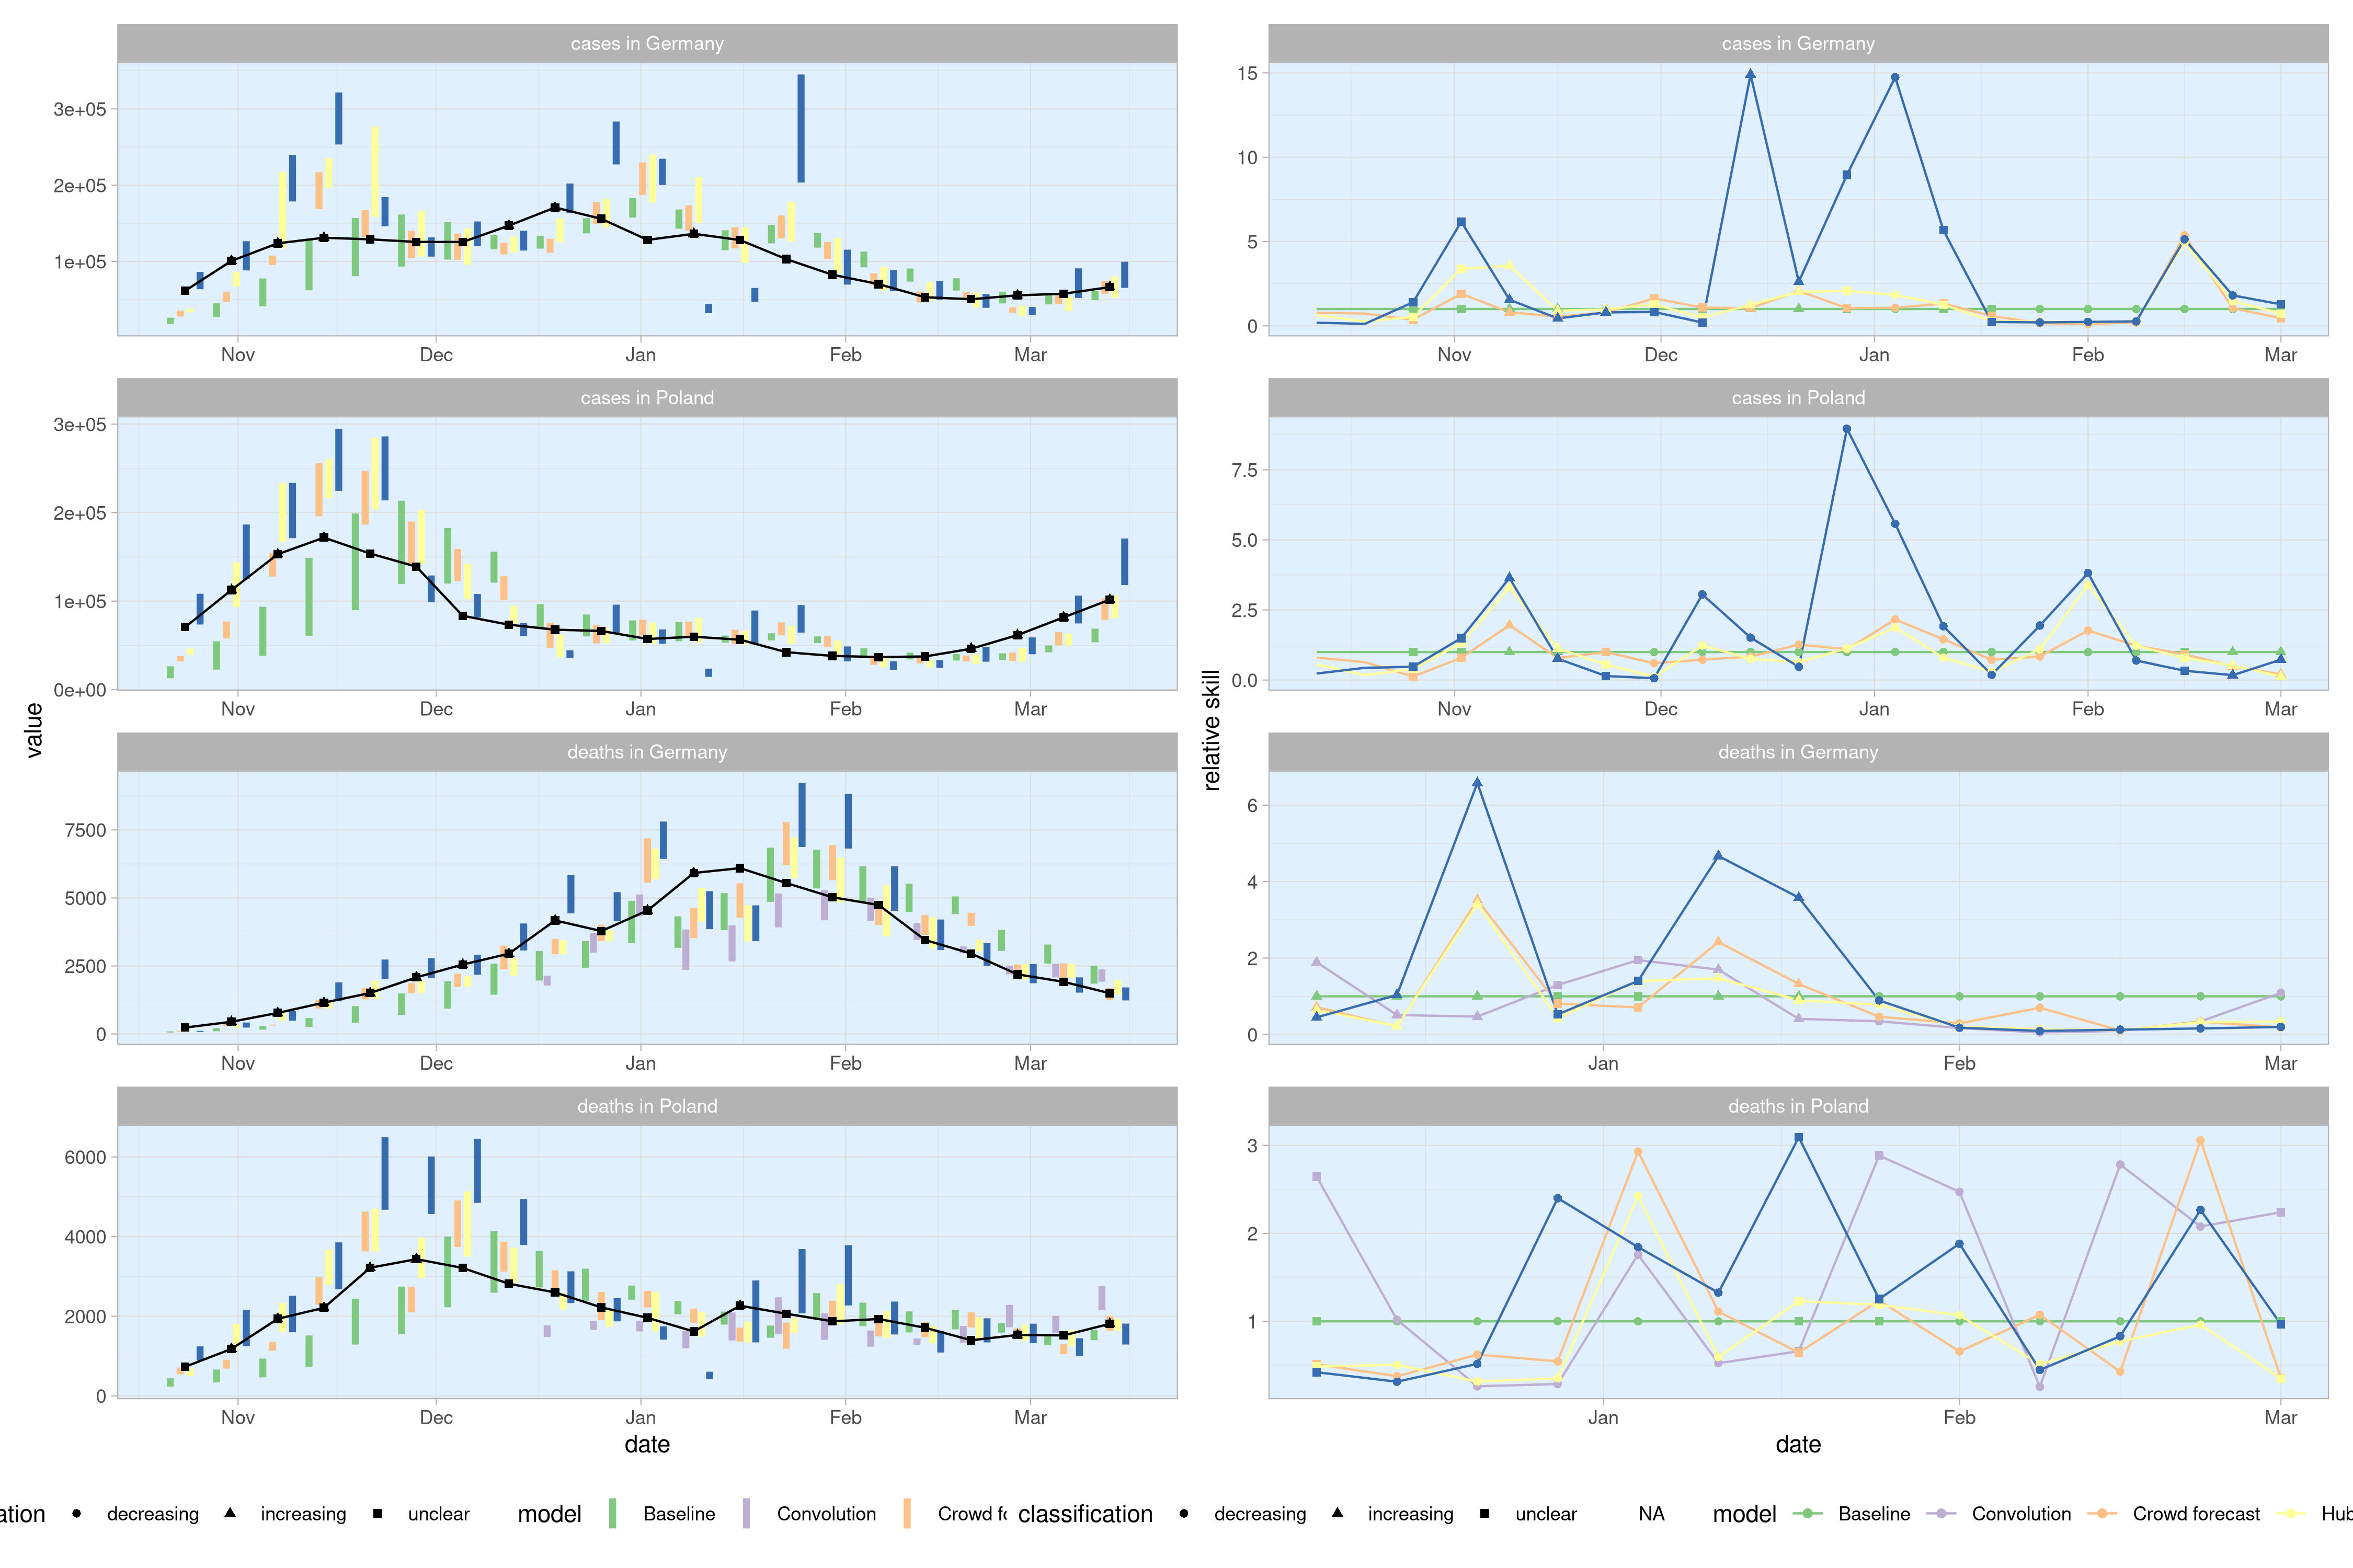
\includegraphics[width=1\linewidth,]{../analysis/plots/figure-forecasts-2} \caption{A, C: Visualisation of 50\% prediction intervals of two week ahead forecasts against the true observed values. Forecasts that were not scored (because there was no complete set of death forecasts available) are greyed out. B, D: Visualisation of corresponding WIS.}\label{fig:forecasts-and-truth}
\end{figure}

\hypertarget{case-forecasts}{%
\subsection{Case Forecasts}\label{case-forecasts}}

For cases, crowd forecasts had a lower mean weighted interval score (WIS, lower values indicate better performance) than both the renewal model and the Hub ensemble across all forecast horizons (Figure \ref{fig:agg-performance-all}A) and locations (Figure \ref{fig:performance-locations-rel}A). For two week ahead forecasts, mean WIS relative to the Hub ensemble (= 1) was 0.89 for crowd forecasts and 1.40 for the renewal model (Table \ref{tab:score-table-2}). Across all forecasting approaches, locations and forecast horizons, the distribution of WIS values was right-skewed, and average performance was heavily influenced by outliers (Figure \ref{fig:distribution-scores}). Overall, low variance in forecast performance was closely linked with good mean performance (Figures \ref{fig:agg-performance-all}H and and \ref{fig:agg-performance-all}A), suggesting that the ability to avoid large errors was an important factor in determining overall performance. The impact of outlier values was especially pronounced for the renewal model, which had more outliers (Figure \ref{fig:distribution-scores}, as well as the highest standard deviation of WIS values (relative WIS sd 1.54 at the two weeks ahead horizon), while the ensemble of crowd forecasts (rel. WIS sd 0.76) and the Hub ensemble (= 1) showed more stable performance.

To varying degrees, all models exhibited trend-following behaviour and were rarely able to predict a change in trend before it had happened. For example, all models failed to predict the change in trend from increase to decrease that happened in early November\ldots{} in Germany and severely overshot (Figure \ref{fig:forecasts-and-truth}A). This was most striking for the renewal model, which extrapolated unconstrained exponential growth based on the recent past of observations. The Hub ensemble and the crowd forecast, which had both been under-predicting throughout October, also failed to predict the change in trend after cases peaked, but less severely so. Human forecasters, possibly aware of the semi-lockdown announced on November 2nd 2020 (Deutsche Welle (www.dw.com) n.d.) and the change in the testing regime (with stricter test criteria) on November 11th 2020 (Ärzteblatt 2020), were fastest to adapt to the new trend, and the Hub ensemble slowest. In December, cases rose again in Germany, with all models under-predicting this growth to varying extents. As in October, the renewal model captured the phase of exponential growth in cases slightly better than other approaches, but again overshot when reported case numbers fell over Christmas. The large variance in predictions in January in Germany (severe under-prediction followed by severe over-prediction) may in part be caused by the fact that the renewal model operated on daily data and therefore was susceptible to fluctuations in daily reporting around Christmas that would not have influenced on weekly reporting. Similar trends in performance were evident in Poland, with the crowd forecast quickest at adapting to the change in trend in November. In general, there were fewer large outlier forecasts in Poland and in particular the renewal model performed more in line with other forecasts there.

All forecasting approaches, including the Hub ensemble, were overconfident and showed lower than nominal coverage (meaning that 50\% (90\%) prediction intervals generally covered less than 50\% (90\%) of the actually observed values) (Figure \ref{fig:agg-performance-all}C and \ref{fig:agg-performance-all}D). Coverage for all forecasts deteriorated with increasing forecast horizon, indicating that all forecasting approaches struggled to quantify uncertainty appropriately for case forecasts. This was especially an issue for crowd forecasts, which were markedly sharper (i.e., narrower) than other approaches (Figure \ref{fig:agg-performance-all}E) and only showed a small increase in uncertainty across forecast horizons. In spite of good performance in terms of the absolute error (Figure \ref{fig:agg-performance-all}G), excessive sharpness led to forecasts which were severely overconfident (covering only 36\% and 55\% of observations with their 50\% and 90\% prediction intervals at a two week horizon, and only 5\% and 38\% four weeks ahead) (Figure \ref{fig:agg-performance-all}C,D and Tables \ref{tab:score-table-2} and \ref{tab:score-table-4}). Despite worse performance in terms of absolute error (Figure \ref{fig:agg-performance-all}G), the renewal model achieved better calibration (comparable to the Hub ensemble), as uncertainty increased rapidly and non-linearly across forecast horizons.

The renewal model exhibited a noticeable tendency towards over-predicting reported cases across all horizons. The crowd forecast tended to over-predict at longer forecast horizons, whereas the Hub ensemble showed no systematic bias (Figure \ref{fig:agg-performance-all}F). Regardless of a general relative tendency to over-predict, all forecasting approaches incurred larger absolute penalties from over- than from under-prediction (see decomposition of the WIS into absolute penalties for over-prediction, under-prediction and dispersion in Figures \ref{fig:agg-performance-all}A and \ref{fig:agg-performance-all}B and Tables \ref{tab:score-table-2} and \ref{tab:score-table-4}), implying that over-prediction (e.g.~when missing a peak) tended to be more costly in terms of the WIS.

Generally, trends in overall performance were broadly similar across locations (Figures \ref{fig:performance-locations} and \ref{fig:performance-locations-rel}).
Due to the differing population sizes and numbers of notifications in Germany and Poland absolute scores were difficult to compare directly. However, relative to the Hub ensemble, the crowd forecasts performed noticeably better in Germany than in Poland and the renewal model better in Poland than in Germany (Figure \ref{fig:performance-locations-rel}A and \ref{fig:performance-locations-rel}G).

\hypertarget{death-forecasts}{%
\subsection{Death Forecasts}\label{death-forecasts}}

For deaths, the Hub ensemble outperformed the crowd forecasts as well as our model-based approaches across all forecast horizons and locations (Figure \ref{fig:agg-performance-all}B, Figure \ref{fig:performance-locations}B). Relative WIS values for the models two weeks ahead were 1.22 (convolution model), 1.26 (crowd forecast), 1 (Hub ensemble) and 1.79 (renewal model). The crowd forecasts performed better than the renewal model across all forecast horizons and locations (Figure \ref{fig:agg-performance-all}B, Figure \ref{fig:performance-locations}B), and also better than the convolution model three and four weeks ahead. Poor performance of the renewal model, especially at longer horizons, indicates that an approach that does not know about past cases, but instead estimates and projects a separate \(R_t\) trace from deaths, is not well suited for the task. The convolution model was able to outperform both the renewal model and the crowd forecasts at shorter forecast horizons (where the delay between cases and deaths means that future deaths are largely informed by present cases), but saw performance deteriorate at three and four weeks ahead (where case predictions from the renewal model were increasingly used to inform death predictions) (Figure \ref{fig:agg-performance-all}B, Table \ref{tab:score-table-4}).

Theoretical considerations suggest that predicting a change in trend may be easier for deaths than for cases (as past cases, hospitalisations and other data can be used as predictors). Even though all forecasts generally struggled with this, there were some instances where changing trends were well captured or even anticipated. In Poland, for example, the Hub ensemble was able to capture or even anticipate the peak in deaths in December quite well (whereas the renewal model and crowd forecast did not). The renewal model, which mostly exhibited trend-following behaviour, correctly predicted another increase in weekly deaths in mid-January (potentially based on changes in daily deaths, as the renewal model did not know about past cases). In Germany in early January, all models predicted a decrease in deaths two to three weeks before it actually happened. Predictions from the renewal model at that time were likely strongly influenced by an unexpected drop in reported deaths on December XXth. The other forecasting approaches and in particular, the convolution model may have been affected by potentially under-reported case numbers around Christmas. When the decrease that all models had predicted to happen in early January failed to materialise, the renewal model and the crowd forecast noticeably over-corrected and over-predicted deaths in the following weeks, while the Hub ensemble, and to a slightly lesser degree, the convolution model were able to capture the downturn well when it finally happened at the end of January.

Death forecasts, generally, showed greater coverage of the 50\% and 90\% prediction intervals than case forecasts and no decrease in coverage across forecast horizons, indicating that it might be easier to appropriately quantify uncertainty for death forecasts. The Hub ensemble had the greatest coverage, with empirical coverage of the 50\% and 90\% prediction intervals exceeding 50\%, and 90\%, respectively, across all forecast horizons. Coverage for the crowd forecasts and our model-based approaches was generally lower than that of the Hub ensemble and mostly slightly lower than nominal coverage (Figure \ref{fig:agg-performance-all}C and \ref{fig:agg-performance-all}D). As for cases, the crowd forecast tended to be the sharpest and uncertainty increased most slowly across forecast horizons, and the renewal model forecasts generally were widest. The convolution model was relatively sharp for short forecast horizons, but had rapidly (and non-linearly) increasing uncertainty for longer forecast horizons, driven by increasing uncertainty in the underlying case forecasts.

For deaths, the ensemble of crowd forecasts had a consistent tendency to over-predict \ref{fig:agg-performance-all}F. The convolution model had a strong tendency to under-predict, which steadily decreased for longer forecast horizons. The renewal model (which over-predicted for cases) and the Hub ensemble slightly tended towards under-prediction. For deaths, absolute over- and under-prediction penalties were more in line with a general relative tendency to over- or under-predict than for cases (Figure \ref{fig:agg-performance-all}A, \ref{fig:agg-performance-all}B and Tables \ref{tab:score-table-2}, \ref{tab:score-table-4}).

\begin{figure}[H]
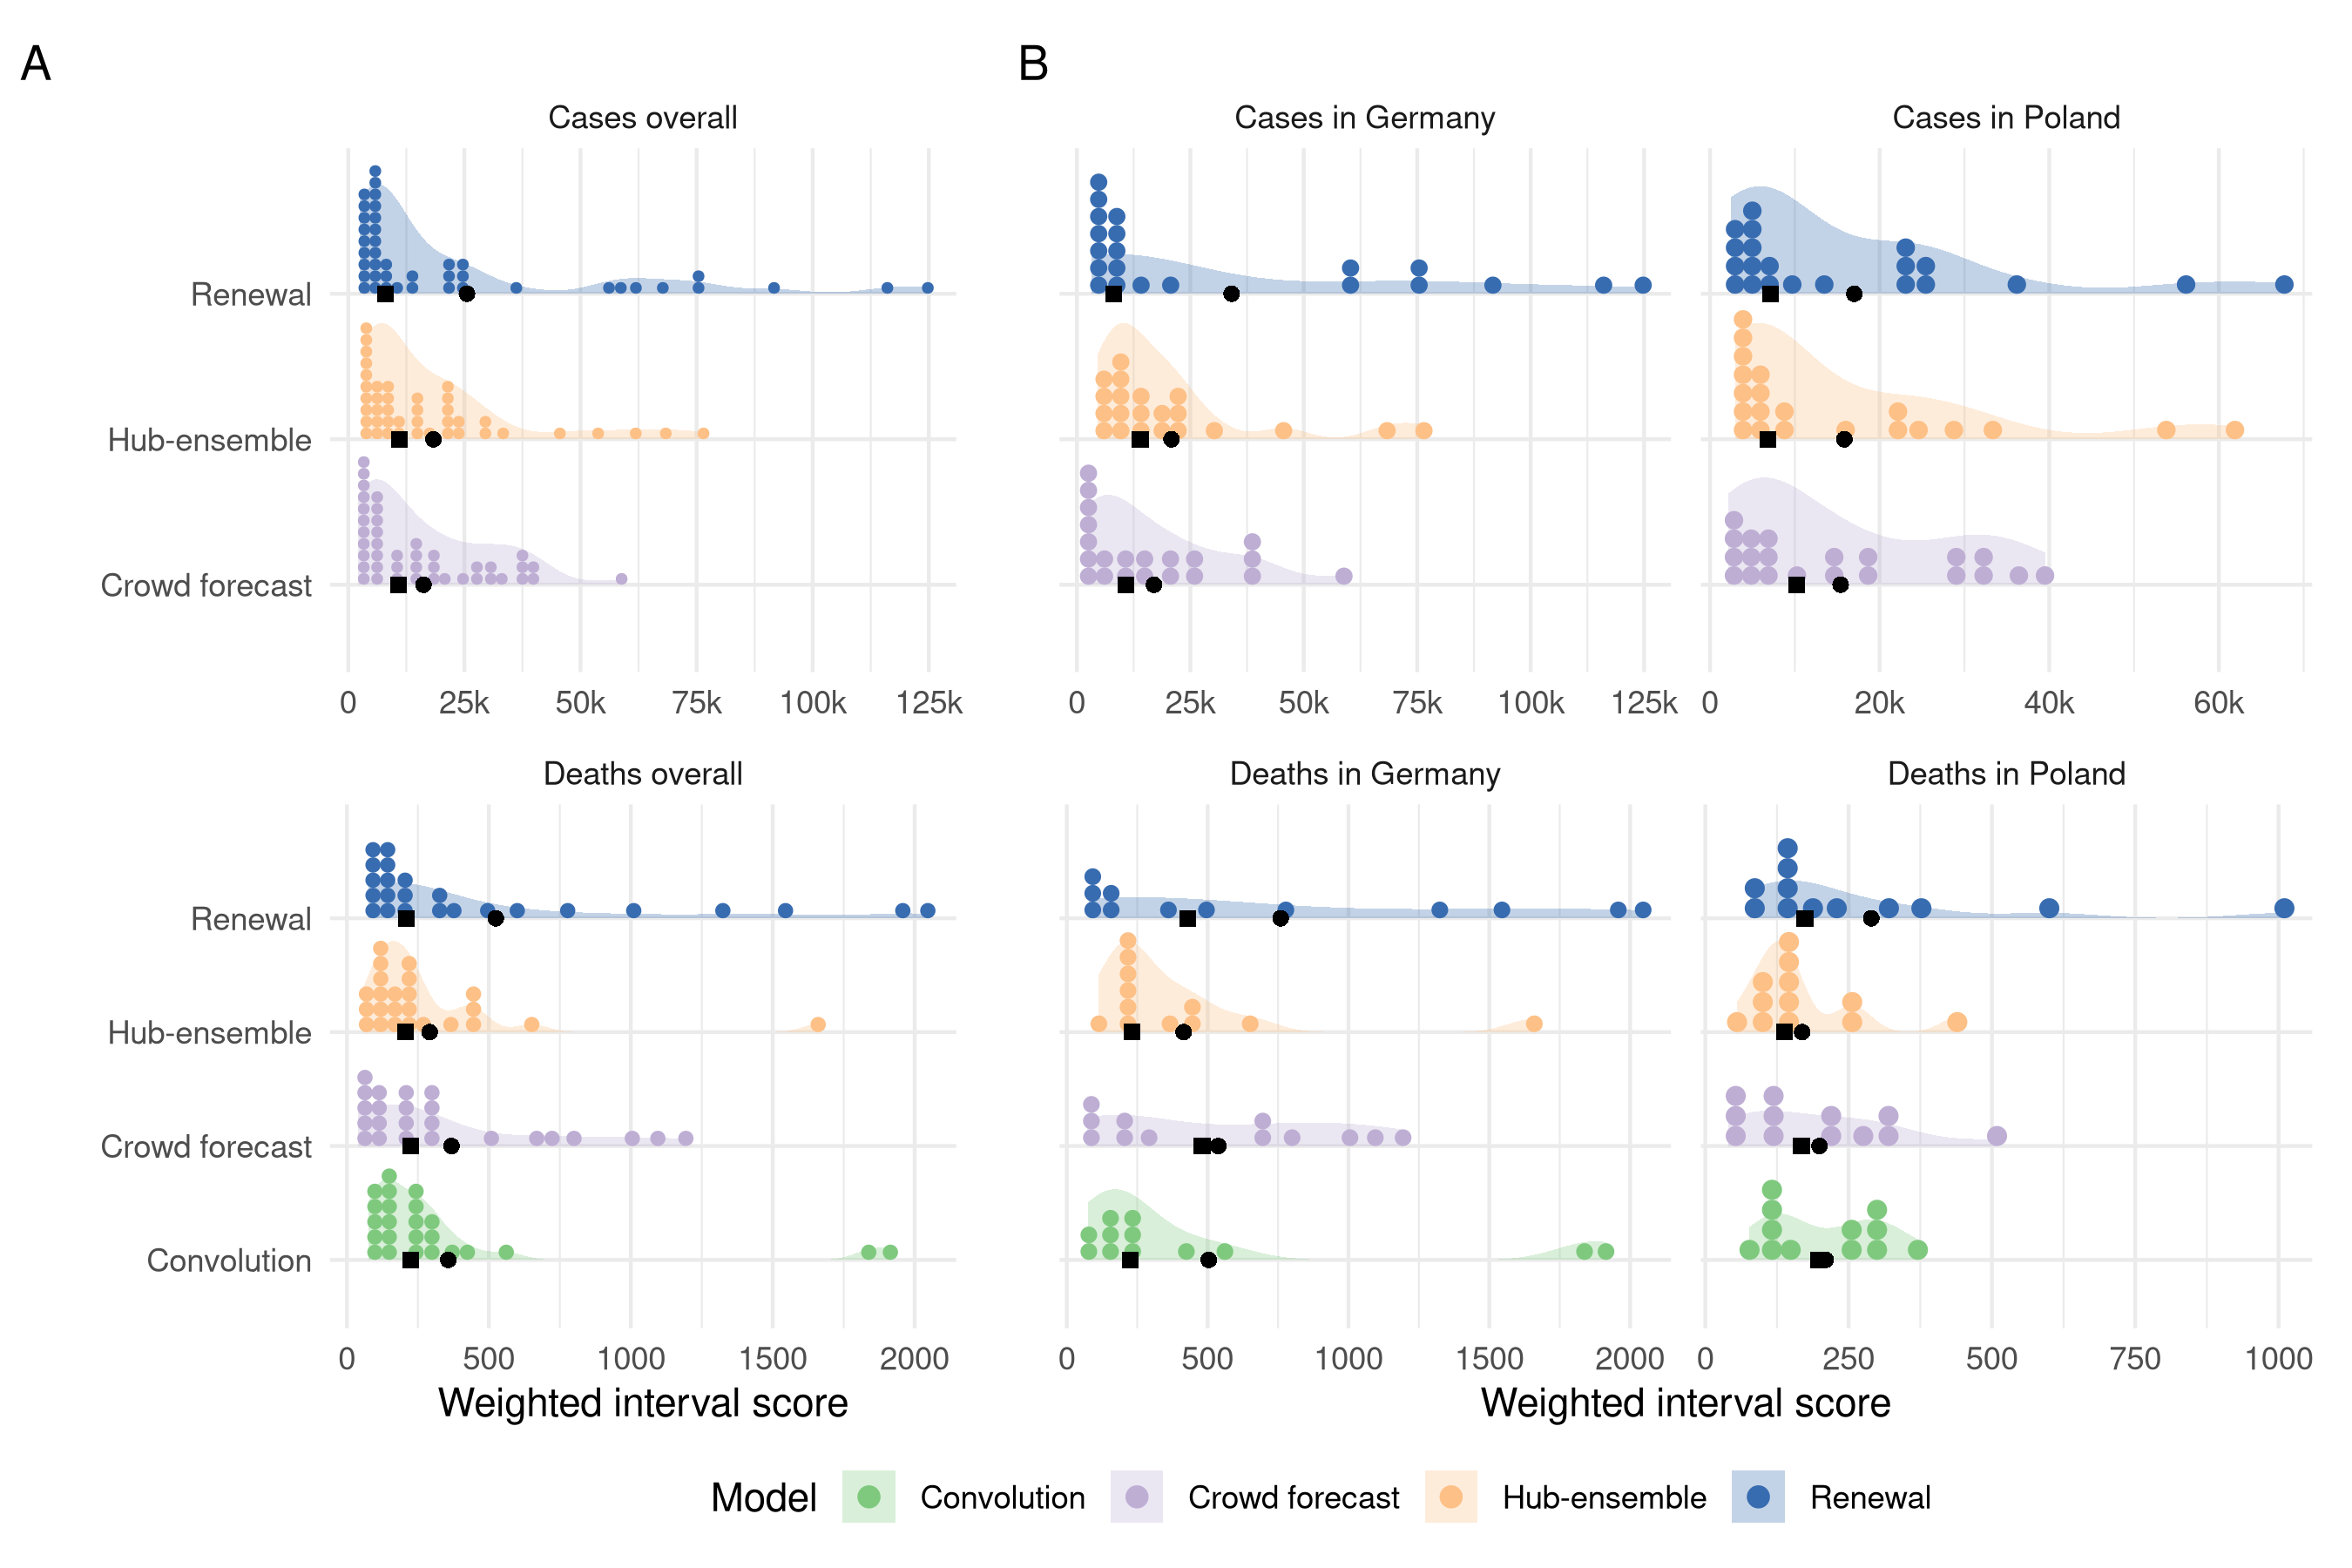
\includegraphics[width=1\linewidth,]{../analysis/plots/distribution_scores_wis-2} \caption{A: Distribution of weighted interval scores for two week ahead forecasts of the different models and forecast targets. B: Distribution of WIS separate by country.}\label{fig:distribution-scores}
\end{figure}

\begin{figure}[H]
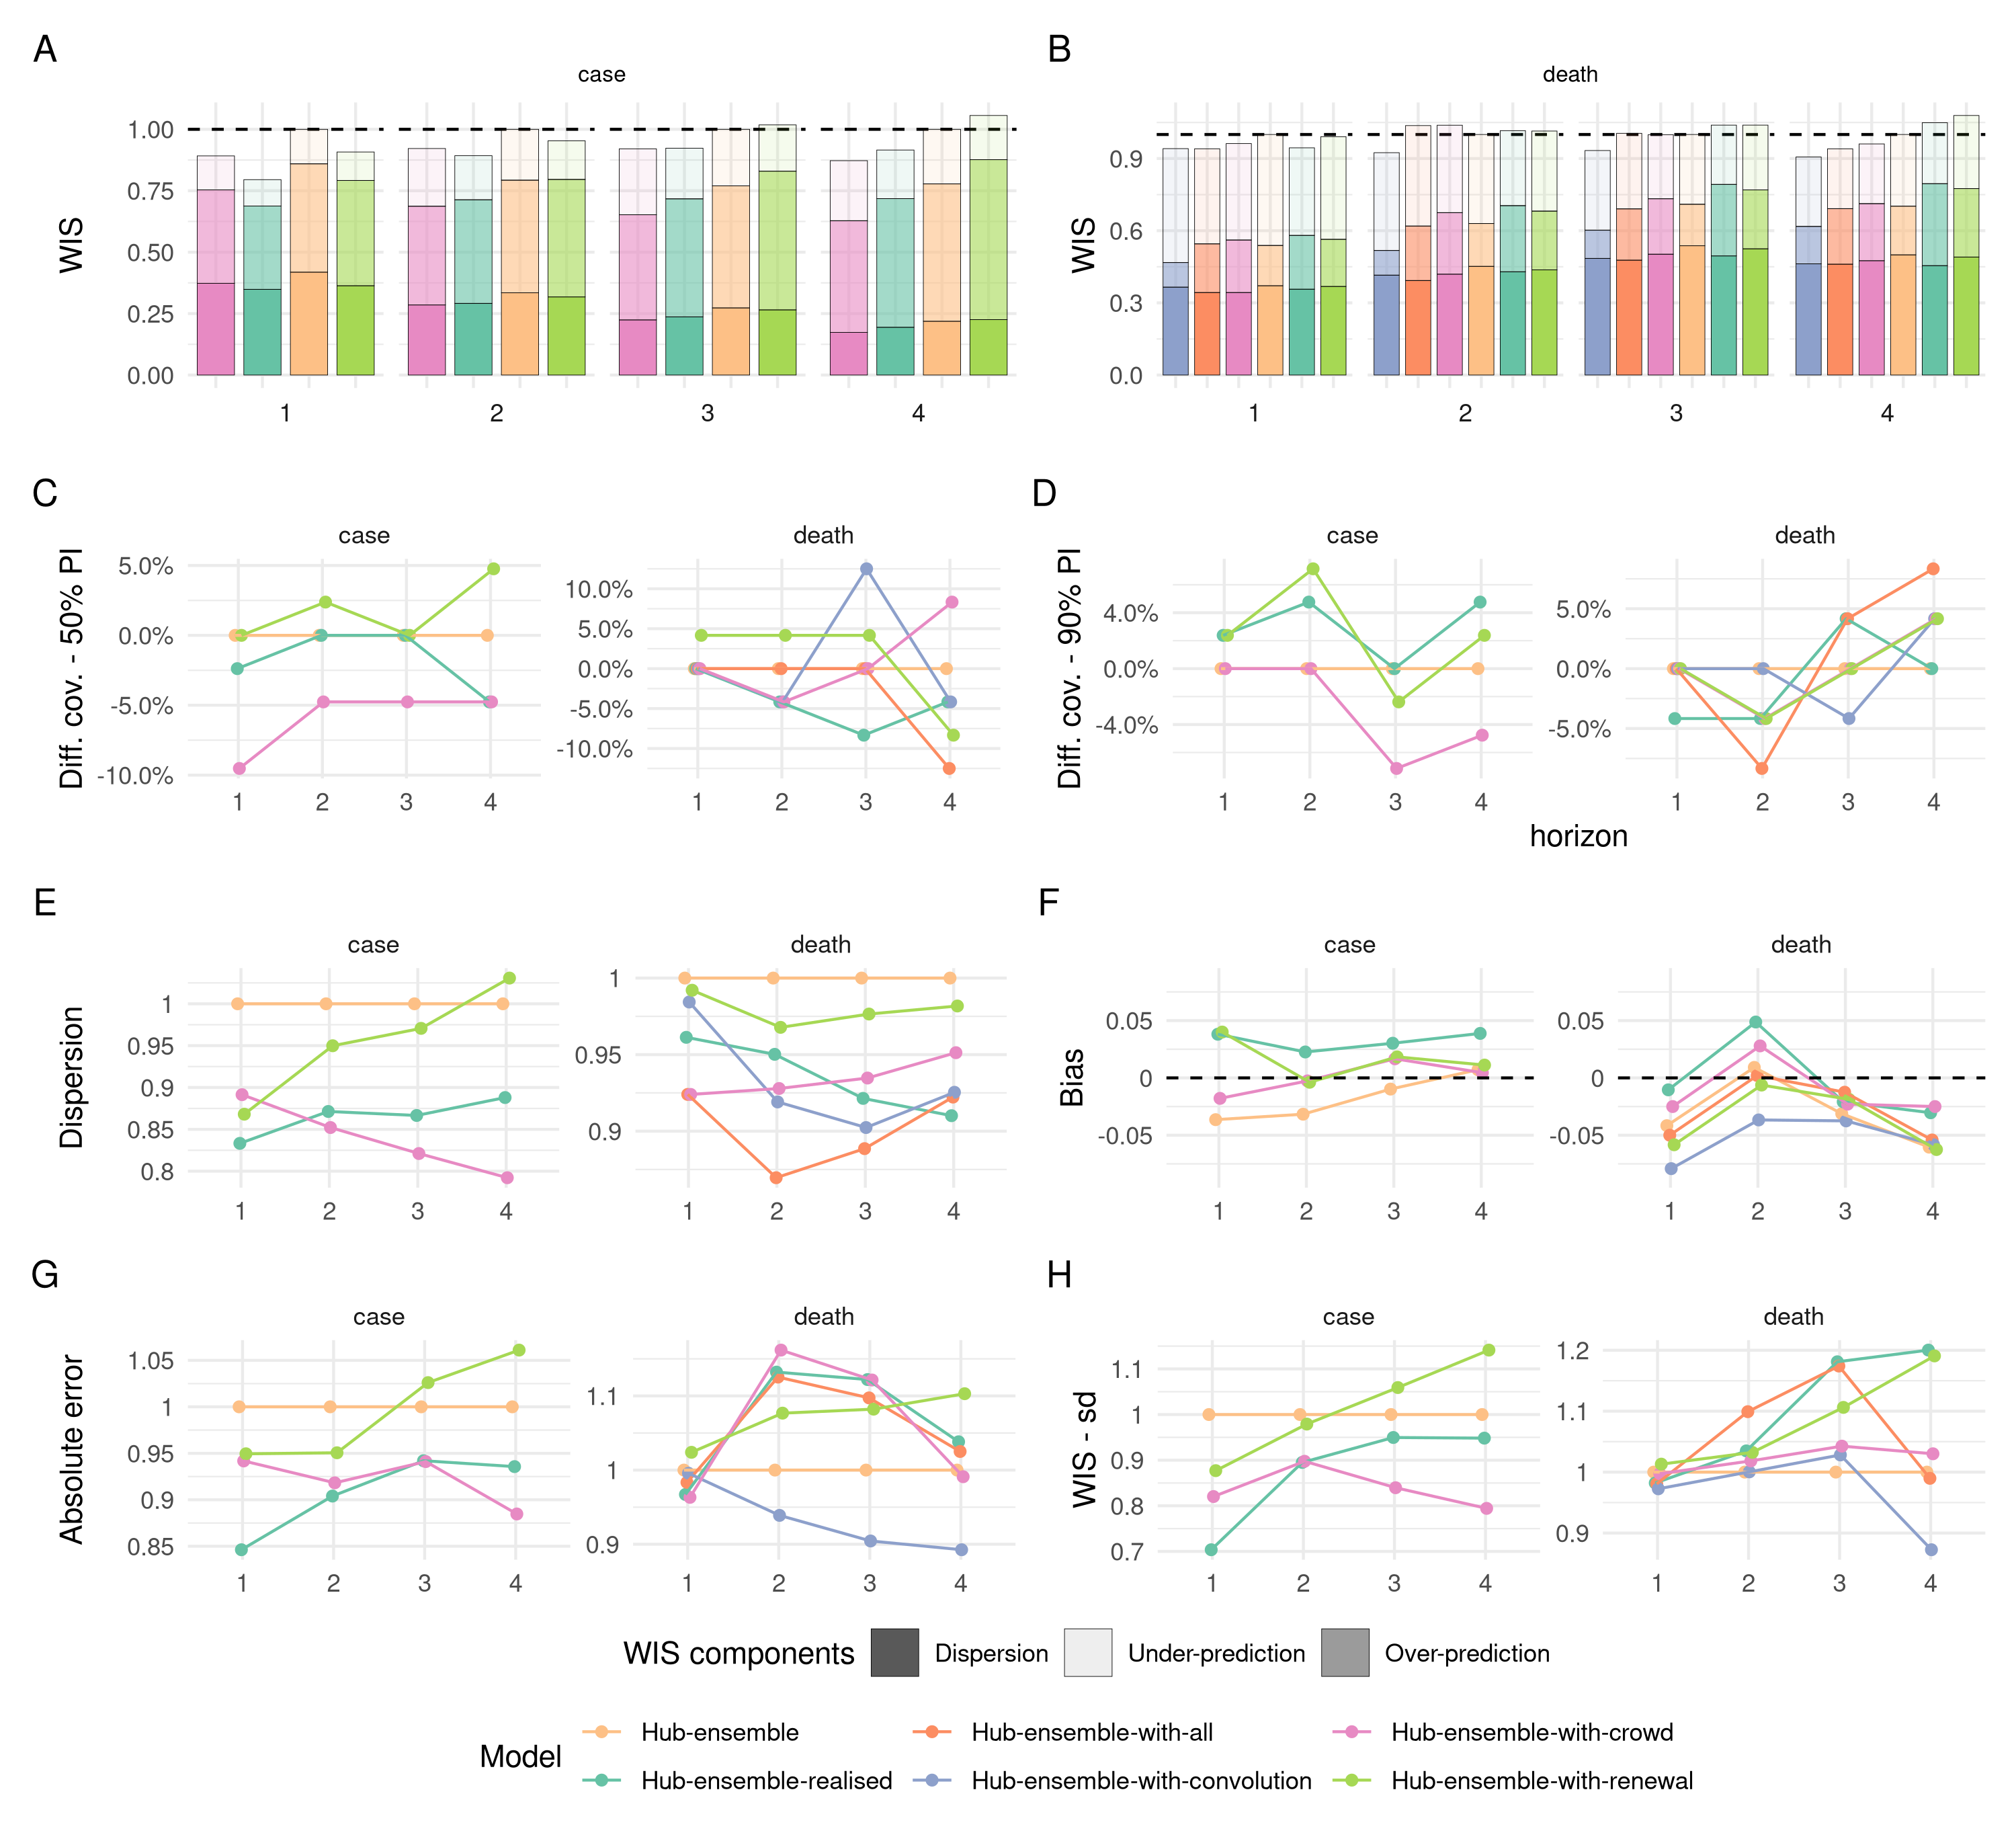
\includegraphics[width=1\linewidth,]{../analysis/plots/aggregate-performance-rel-ensemble-v4} \caption{Visualisation of aggregate performance metrics across forecast horizons for the different versions of the Hub median ensemble. “Hub-ensemble” excludes all our models, Hub-ensemble-all includes all of our models, “Hub-ensemble-real” is the real hub-ensemble with the renewal model and the crowd forecasts included. Values (except for Bias) are computed as differences to the Hub ensemble excluding our contributions. For Coverage, this is an absolute difference, for other metrics this is a percentage difference. A: mean weighted interval score (WIS) across horizons. B: median WIS. C: Absolute error of the median forecast. D: Standard deviation of the WIS. E: Dispersion (higher values mean greater spread of the forecast). F: Bias, i.e. general tendency to over- or underpredict. Values are between -1 (complete under-prediction) and 1 (complete over-prediction) and 0 ideally. G: Empirical coverage of the 50\% prediction intervals. F: Empirical coverage of the 90\% prediction intervals}\label{fig:agg-performance-ensemble}
\end{figure}

\hypertarget{contribution-to-the-forecast-hub}{%
\subsection{Contribution to the Forecast Hub}\label{contribution-to-the-forecast-hub}}

Of our three models, only the renewal model and the crowd forecast were included in the official Forecast Hub median ensemble (``hub-ensemble-realised''), while the convolution model was never included as it was deemed too similar to the existing renewal model, thus potentially introducing bias. In the official Hub ensemble, there were on average 7.1 models included (including our own), with a median of 7, a minimum of 4 (on December 28 2020 over the Christmas period) and a maximum of 10. Versions that included either all of our models (``hub-ensemble-with-all'') or only one of them (``hub-ensemble-with-X'') were computed retrospectively. An overview of all models and ensemble versions is shown in Table \ref{tab:table-ensemble-versions} in the SI.

For cases, our contributions (compared to the Hub ensemble without our contributions) consistently improved performance across all forecasting horizons (rel. WIS 0.9 two weeks ahead, Table \ref{tab:score-table-ensemble-2}). Contributions from the crowd forecasts alone also were positive across all forecast horizons, while contributions from the renewal model became negative for longer horizons (rel. WIS 1.02 three weeks ahead, 1.06 four weeks ahead). The realised ensemble including both models performed better or equal compared to all versions with only one model included for up to three weeks ahead, suggesting synergistic effects. Only for four week ahead predictions would removing the renewal model have improved performance (Table \ref{tab:score-table-ensemble-4}).

For deaths, contributions from the renewal model and crowd forecast together improved performance only for one week ahead predictions and showed an increasingly negative impact on performance for longer horizons (rel. WIS of the hub-ensemble-realised 1.01 two weeks ahead, 1.05 four weeks ahead, Tables \ref{tab:score-table-ensemble-2} and \ref{tab:score-table-ensemble-4}). Individual contributions from both the renewal model and the crowd forecast were largely negative, while a version of the Hub ensemble with only the convolution model included would have performed consistently better across all forecast horizons (with the positive impact increasing for longer horizons). This is especially interesting as the convolution model performed consistently worse than the pre-existing Hub ensemble (Figure \ref{fig:agg-performance-all}) and especially worse for longer horizons.

We also considered the impact of our contributions on the mean, rather than the median ensemble.
General trends were similar, with the notable exception of the convolution model, which had a consistently positive impact on the median ensemble, but a mixed and mostly slightly negative impact on the mean ensemble (Figures \ref{fig:agg-performance-ensemble}B and \ref{fig:agg-performance-ensemble-mean}B). This may happen if a model is more correct directionally relative to the pre-existing ensemble, but overshoots in absolute terms, thereby moving the ensemble too far. For both the mean and the median ensemble, changes in performance from adding or removing models were of a similar order of magnitude, suggesting that at least in this instance, with a relatively small ensemble size, the median ensemble was not necessarily more `robust' to changes than the mean ensemble. However, the ensemble version with all our forecasts included (``hub-ensemble-with-all'') tended to perform relatively better for the median ensemble than the mean ensemble, suggesting that adding more models may be more beneficial or `safer' for the median than for the mean ensemble as directional errors can more easily cancel out than errors in absolute terms.

\hypertarget{discussion}{%
\section{Discussion}\label{discussion}}

Epidemiological forecasting usually represents a mix between human insight and model-based assumptions. In this study, we compared purely opinion-derived forecasts of cases and deaths from COVID-19 in Germany and Poland, elicited from a crowd of researchers and volunteers against predictions from two semi-mechanistic epidemiological models. In spite of the small number of participants and a general tendency to be overconfident, crowd forecasts consistently outperformed our epidemiological models as well as the Hub ensemble when forecasting cases but not when forecasting deaths. This suggests that humans are relatively good at foreseeing trends that are hard to model but may struggle to form an intuition for the exact relationship between cases and deaths.

Past studies have evaluated the performance of model-based forecasting approaches as well as human experts and non-experts in various contexts. However, most of these studies either focused only on the evaluation of (expert-tuned) model-based approaches (e.g. Funk et al. 2020; Cramer et al. 2020; Cramer et al. 2021), or exclusively on human forecasts Recchia, Freeman, and Spiegelhalter (2021). In contrast, we directly compared human and model-based forecasts. This is similar to the approach taken by Farrow et al. (2017), but extends it in several ways. While Farrow et al.~only asked for point predictions and constructed a probabilistic forecast from these, we asked participants to quantify their uncertainty directly, allowing us to compare human forecasts and models without any further assumptions, as well as to analyse aspects of the forecasts like overconfidence. In addition, we compared crowd forecasts to two semi-mechanistic models informed by basic epidemiological knowledge of COVID-19, allowing us to assess not only relative performance but also to analyse qualitative differences between human judgement and model-derived insight. In terms of interpretability of the results, exact knowledge of our two models, as well as focus on a limited set of targets and locations was a major advantage of our study compared to larger studies conducted by the Forecast Hubs (Cramer et al. 2020; Cramer et al. 2021; Bracher, Wolffram, et al. 2021; Hub 2021; Funk et al. 2020).

The good performance of crowd forecasts we found is in line with results from Farrow et al.~who also report strong performance of human predictions in past Flu challenges despite difficulties to recruit a large number of participants. The advantage of crowd forecasts we observed over our semi-mechanistic models is likely in part explained by the fact that we compared an ensemble of crowd forecasts with single models. However, this probably explains only part of the difference and performance relative to the Hub ensemble strongly suggests that human insight is valuable when predicting highly volatile and hard-to-predict quantities such as case numbers. Relatively good performance of our semi-mechanistic models short-term, but not longer-term, suggests that model-based forecasts are helpful to extrapolate from current conditions, but require some form of human intervention or additional assumptions to inform forecasts when conditions change over time. This human intervention may be particularly important when dealing with artefacts in reporting and data anomalies (and especially when using daily, rather than weekly data). The large variance in predictions in January in Germany for example (severe under-prediction followed by severe over-prediction, see Figure \ref{fig:forecasts-and-truth}A), may in part be caused by the fact that the renewal model operated on daily data and therefore was susceptible to fluctuations in daily reporting around Christmas that would not have influenced on weekly reporting. While we were not able to observe how expert opinion informed other models submitted to the Forecast Hub, conversations with the Hub organisers suggest that forecasts tended to benefit from a large degree of human intervention. Unfortunately, we were not able to test a scenario in which users were asked to alter an existing model output. We can therefore make no conclusive statements about the direct effects of researchers tuning their models, rather than create a new forecast from a naive baseline.

Conversely, our results suggest that human intervention may be less beneficial when forecasting deaths (especially at shorter horizons, when deaths are largely dependent on already observed cases), which benefits from the ability to model the delays and exact epidemiological relationships between different leading and lagged indicators. Relatively good performance of the convolution model, especially compared to the poor performance of the renewal model on deaths (which used only deaths to estimate and predict the effective reproduction number) underlines the importance of including leading indicators such as cases as a predictor for deaths.

Given the low number of participants in our study, it is difficult to generalise conclusions about crowd predictions to other settings. In particular, our crowd forecasting application was not developed to a high standard of user friendliness. This may have precluded interested parties from submitting forecasts. The low number of participants presumably resulted in higher variance of forecasts, but also potentially in better average forecast performance. Motivating forecasters to contribute regularly proved challenging, especially given that the majority of our participants were from the UK and had little connection to Germany and even less to Poland. In addition, lack of effective outreach played an important role, as did a lack of time and resources to design the interface in a way that is appealing enough to attract large audiences outside of academia. Using an R shiny app as an interface arguably created some limits to user experience and performance, influencing the number of participants. On the other hand, it facilitated quick development and allows us to provide our crowd forecasting tooling as an open source R package, meaning that it is available for others to use, and to further develop, in their context.

In general, our results support the use of ensembles, rather than individual models to inform public health policies, as these provide consistently good performance and largely avoid particularly bad outlier forecasts. Our results also suggest that at least for a small median ensemble like the German and Polish Forecast Hub ensemble adding more models may increase performance in most instances (with the version of the hub ensemble that includes all our contributions (``hub-ensemble-with-all'') outperforming the realised official hub ensemble in almost all instances). We often found contributions to an ensemble to be beneficial even in instances where the forecasting approach entering the ensemble performed consistently worse than the pre-existing ensemble. Including more models may be easier when using a median ensemble, as extreme forecasts tend to have less of an influence there. Individual models, however, can still have a place in informing public policy. As an average, ensembles show the consensus opinion, which implies that in contrast to single models, they are not likely to reveal information, e.g.~about future changes in trend, that is not in some way `obvious' to the majority of forecasters.

In the context of evaluating different models and the merits of human intervention, what constitutes a `good' forecast very much depends on the purpose of that forecast. Policymakers may care much more about certain types of errors, (e.g.~under-prediction) than others in a way not captured by the weighted interval score. Also, it is helpful to distinguish between `forecasts' and `projections.' For example, the outperformance of the crowd forecasts on cases and in general on longer forecast horizons is perhaps not surprising, given that humans could factor in an expectation of future changes in conditions (e.g.~future policy interventions, adherence to these interventions, testing policy, and the evolution of new disease variants) while our model-based forecasts could not. However, if the aim of a forecast is to inform policy and decision making, then attempting to factor in the interventions one is meant to inform may be problematic (and conversely, arguing for or against interventions based on predictions may be difficult depending on what the forecast assumes about future interventions). In that sense, crowd forecasts can be understood as forecasts, whereas our model predictions may be better understood as projections that show what would happen in the absence of any events that could change the trend. This may pose a problem in the context of a forecast hub if teams have a different understanding about the purpose of a forecast. Projections that are meant to inform policy makers about possible scenarios may be different from forecasts meant to inform the general public, and yet again different from forecasts submitted with the goal of advancing open research and in order to allow public scrutiny and discussion about the merits of different approaches.

Further work should explore the effects of human intervention on model-based forecasts in more detail. Model-based forecasts could be used as an input to human judgement, with researchers adjusting predictions generated by models. Seeing a model-based forecasts could help humans calibrate uncertainty better, while allowing for manual intervention to adapt spurious trend predictions. Tools need to be developed to facilitate this process at a larger scale. Human insight could also be used as an input to models. Such a `hybrid' forecasting approach could for example ask humans to predict the trend of the effective reproduction number \(R_t\) or the doubling rate (i.e.~how the epidemic evolves) into the future and use this to estimate the exact number of cases, hospitalisations or deaths this would imply. This approach seems especially promising for forecasting deaths if a model can accurately describe delay distributions and epidemiological relationships between different parameters. In light of severe overconfidence, yet good performance in terms of the absolute error, post-processing of human forecasts to adjust and widen confidence intervals may be another promising approach. Crowd forecasting in general could benefit greatly from the availability of tools suitable to appeal to a greater audience. Given the good performance we and previous authors observed in spite of the limited resources available and the small number of participants, this seems worthwhile for researchers and policymakers to further develop and explore.

\hypertarget{appendix-supplementary-information}{%
\appendix}


\hypertarget{supplementary-information}{%
\section{Supplementary information}\label{supplementary-information}}

\hypertarget{scoring-metrics-used}{%
\subsection{Scoring metrics used}\label{scoring-metrics-used}}

\begin{longtable}[t]{>{\raggedright\arraybackslash}p{2.5cm}>{\raggedright\arraybackslash}p{13.0cm}}
\caption{\label{tab:scoring-metrics}Overview of the scoring metrics used.}\\
\toprule
Metric & Explanation\\
\midrule
\endfirsthead
\caption[]{\label{tab:scoring-metrics}Overview of the scoring metrics used. \textit{(continued)}}\\
\toprule
Metric & Explanation\\
\midrule
\endhead

\endfoot
\bottomrule
\endlastfoot
WIS (Weighted) interval score & The weighted interval score (smaller values are better) is a proper scoring rule for quantile forecasts. It converges to the continuos ranked probability score (which itself is a generalisation of the absolute error to probabilistic forecasts) for an increasing number of intervals. The score can be decomposed into a dispersion (uncertainty) component and penalties for over- and underprediction. For a single interval, the score is computed as 
  $$IS_\alpha(F,y) = (u-l) + \frac{2}{\alpha} \cdot (l-y) \cdot 1(y \leq l) + \frac{2}{\alpha} \cdot (y-u) \cdot 1(y \geq u), $$ 
  where $1()$ is the indicator function, $y$ is the true value, and $l$ and $u$ are the $\frac{\alpha}{2}$ and $1 - \frac{\alpha}{2}$ quantiles of the predictive distribution $F$, i.e. the lower and upper bound of a single prediction interval. For a set of $K$ prediction intervals and the median $m$, the score is computed as a weighted sum, 
  $$WIS = \frac{1}{K + 0.5} \cdot (w_0 \cdot |y - m| + \sum_{k = 1}^{K} w_k \cdot IS_{\alpha}(F, y)),$$ 
  where $w_k$ is a weight for every interval. Usually, $w_k = \frac{\alpha_k}{2}$ and $w_0 = 0.5$. 

\cellcolor{gray!6}{Its proximity to the absolute error means that when averaging across multiple targets (e.g. different weeks), it will be dominated by targets with higher absolute values.}\\
\addlinespace \addlinespace
Interval coverage & Interval coverage is a measure of marginal calibration and indicates the proportion of observed values that fall in a given prediction interval range. Nominal coverage represents the percentage of observed values that should ideally be covered (e.g. we would like a 50 percent prediction interval to cover on average 50 percent of the observations), while empirical coverage is the actual percentage of observations covered by a certain prediction interval.\\
\addlinespace \addlinespace
Bias & (Relative) bias is a measure of the general tendency of a forecaster to over- or underpredict. Values are between -1 and 1 and 0 ideally. For continuous forecasts, bias is given as 
$$B(F, y) = 1 - 2 \cdot (F (y)), $$ 
where $F$ is the CDF of the predictive distribution and $y$ is the observed value. 

For quantile forecasts, $F(y)$ is replaced by a quantile rank. The appropriate quantile rank is determined by whether the median forecast is below  or above the true value. We then take the innermost quantile rank for which the quantile is still larger (under-prediction) or smaller (over-prediction) than the observed value. 

\cellcolor{gray!6}{In contrast to the over- and underprediction penalties of the interval score it is bound between 0 and 1 and represents a general tendency of forecasts to be biased rather than the absolute amount of over- and underprediction. It is therefore a more robust measurement.}\\*
\end{longtable}

\clearpage

\hypertarget{further-details-on-the-semi-mechanistic-forecasting-models}{%
\subsection{Further details on the semi-mechanistic forecasting models}\label{further-details-on-the-semi-mechanistic-forecasting-models}}

\hypertarget{renewal-equation-model}{%
\subsubsection{Renewal equation model}\label{renewal-equation-model}}

The model was initialised prior to the first observed data point by assuming constant exponential growth for the mean of assumed delays from infection to case report.

\begin{align*}
  I_{t} &= I_0 \exp  \left(r t \right)  \\
  I_0 &\sim \mathcal{LN}(\log I_{obs}, 0.2) \\
  r &\sim \mathcal{LN}(r_{obs}, 0.2) 
\end{align*}

Where \(I_{obs}\) and \(r_{obs}\) are estimated from the first week of observed data. For the time window of the observed data infections were then modelled by weighting previous infections by the generation time and scaling by the instantaneous reproduction number. These infections were then convolved to cases by date (\(O_t\)) and cases by date of report (\(D_t\)) using log-normal delay distributions. This model can be defined mathematically as follows,

\begin{align*}
  \log R_{t} &= \log R_{t-1} + \mathrm{GP}_t \\
  I_t &= R_t \sum_{\tau = 1}^{15} w(\tau | \mu_{w}, \sigma_{w}) I_{t - \tau} \\
  O_t &= \sum_{\tau = 0}^{15} \xi_{O}(\tau | \mu_{\xi_{O}}, \sigma_{\xi_{O}}) I_{t-\tau} \\
  D_t &= \alpha \sum_{\tau = 0}^{15} \xi_{D}(\tau | \mu_{\xi_{D}}, \sigma_{\xi_{D}}) O_{t-\tau} \\ 
  C_t &\sim \mathrm{NB}\left(\omega_{(t \mod 7)}D_t, \phi\right)
\end{align*}

Where,
\begin{align*}
     w &\sim \mathcal{G}(\mu_{w}, \sigma_{w}) \\
    \xi_{O} &\sim \mathcal{LN}(\mu_{\xi_{O}}, \sigma_{\xi_{O}}) \\
    \xi_{D} &\sim \mathcal{LN}(\mu_{\xi_{D}}, \sigma_{\xi_{D}}) 
\end{align*}

This model used the following priors for cases,

\begin{align*}
     R_0 &\sim \mathcal{LN}(0.079, 0.18) \\
    \mu_w &\sim \mathcal{N}(3.6, 0.7) \\
    \sigma_w &\sim \mathcal{N}(3.1, 0.8) \\
    \mu_{\xi_{O}} &\sim \mathcal{N}(1.62, 0.064) \\
    \sigma_{\xi_{O}} &\sim \mathcal{N}(0.418, 0.069) \\
    \mu_{\xi_{D}} &\sim \mathcal{N}(0.614, 0.066) \\
    \sigma_{\xi_{D}} &\sim \mathcal{N}(1.51, 0.048) \\
    \alpha &\sim \mathcal{N}(0.25, 0.05) \\
    \frac{\omega}{7} &\sim \mathrm{Dirichlet}(1, 1, 1, 1, 1, 1, 1) \\
    \phi &\sim \frac{1}{\sqrt{\mathcal{N}(0, 1)}}
\end{align*}

and updated the reporting process as follows when forecasting deaths,

\begin{align*}
    \mu_{\xi_{D}} &\sim \mathcal{N}(2.29, 0.076) \\
    \sigma_{\xi_{D}} &\sim \mathcal{N}(0.76, 0.055) \\
    \alpha &\sim \mathcal{N}(0.005, 0.0025) 
\end{align*}

\(\alpha\), \(\mu\), \(\sigma\), and \(\phi\) were truncated to be greater than 0 and with \(\xi\), and \(w\) normalised to sum to 1.

The prior for the generation time was sourced from (Ganyani et al. 2020) but refit using a log-normal incubation period with a mean of 5.2 days (SD 1.1) and SD of 1.52 days (SD 1.1) with this incubation period also being used as a prior (Lauer et al. 2020) for \(\xi_{O}\). This resulted in a gamma-distributed generation time with mean 3.6 days (standard deviation (SD) 0.7), and SD of 3.1 days (SD 0.8) for all estimates. We estimated the delay between symptom onset and case report or death required to convolve latent infections to observations by fitting an integer adjusted log-normal distribution to 10 subsampled bootstraps of a public linelist for cases in Germany from April 2020 to June 2020 with each bootstrap using 1\% or 1769 samples of the available data (Xu et al., n.d.; Abbott, Sherratt, et al. 2020) and combining the posteriors for the mean and standard deviation of the log-normal distribution (Abbott, Hellewell, et al. 2020; DOI n.d.; {``Evaluating the Use of the Reproduction Number as an Epidemiological Tool, Using Spatio-Temporal Trends of the {Covid}-19 Outbreak in {England} \textbar{} {medRxiv}''} n.d.; Stan Development Team 2020).

\(GP_t\) is an approximate Hilbert space Gaussian process as defined in (Riutort-Mayol et al. 2020) using a Matern 3/2 kernel using a boundary factor of 1.5 and 17 basis functions (20\% of the number of days used in fitting). The length scale of the Gaussian process was given a log-normal prior with a mean of 21 days, and a standard deviation of 7 days truncated to be greater than 3 days and less than 60 days. The magnitude of the Gaussian process was assumed to be normally distributed centred at 0 with a standard deviation of 0.1.

From the forecast time horizon (\(T\)) and onwards the last value of the Gaussian process was used (hence \(R_t\) was assumed to be fixed) and latent infections were adjusted to account for the proportion of the population that was susceptible to infection as follows,

\begin{equation}
    I_t = (N - I^c_{t-1}) \left(1 - \exp \left(\frac{-I'_t}{N - I^c_{T}}\right)\right),
\end{equation}

where \(I^c_t = \sum_{s< t} I_s\) are cumulative infections by \(t-1\) and \(I'_t\) are the unadjusted infections defined above. This adjustment is based on that implemented in the \texttt{epidemia} R package (Scott et al. 2020; Bhatt et al., n.d.).

\hypertarget{convolution-model}{%
\paragraph{Convolution model}\label{convolution-model}}

The convolution model shares the same observation model as the renewal model but rather than assuming that an observation is predicted by itself using the renewal equation instead assumes that it is predicted entirely by another observation after some parametric delay. It can be defined mathematically as follows,

\begin{equation} 
    D_{t} \sim \mathrm{NB}\left(\omega_{(t \mod 7)} \alpha \sum_{\tau = 0}^{30} \xi(\tau | \mu, \sigma) C_{t-\tau},  \phi \right)
\end{equation}

with the following priors,

\begin{align*}
    \frac{\omega}{7} &\sim \mathrm{Dirichlet}(1, 1, 1, 1, 1, 1, 1) \\
    \alpha &\sim \mathcal{N}(0.01, 0.02) \\
    \xi &\sim \mathcal{LN}(\mu, \sigma) \\
    \mu &\sim \mathcal{N}(2.5, 0.5) \\
\sigma &\sim \mathcal{N}(0.47, 0.2) \\
\phi &\sim \frac{1}{\sqrt{\mathcal{N}(0, 1)}}
\end{align*}

with \(\alpha\), \(\mu\), \(\sigma\), and \(\phi\) truncated to be greater than 0 and with \(\xi\) normalised such that \(\sum_{\tau = 0}^{30} \xi(\tau | \mu, \sigma) = 1\).

\hypertarget{model-fitting}{%
\subsubsection{Model fitting}\label{model-fitting}}

Both models were implemented using the \texttt{EpiNow2} R package (version 1.3.3) (Abbott, Hellewell, et al. 2020). Each forecast target was fitted independently for each model using Markov-chain Monte Carlo (MCMC) in stan (Stan Development Team 2020). A minimum of 4 chains were used with a warmup of 250 samples for the renewal equation-based model and 1000 samples for the convolution model. 2000 samples total post warmup were used for the renewal equation model and 4000 samples for the convolution model. Different settings were chosen for each model to optimise compute time contingent on convergence. Convergence was assessed using the R hat diagnostic (Stan Development Team 2020). For the convolution model forecast the case forecast from the renewal equation model was used in place of observed cases beyond the forecast horizon using 1000 posterior samples. 12 weeks of data was used for both models though only 3 weeks of data were included in the likelihood for the convolution model.

\clearpage

\hypertarget{tables-with-results-of-the-forecast-evaluation}{%
\subsection{Tables with results of the forecast evaluation}\label{tables-with-results-of-the-forecast-evaluation}}

\begin{table}[!h]
\caption{\label{tab:score-table-2}Scores for one and two week ahead forecasts (cut to three significant digits and rounded). Note that scores for cases (which include the whole period from October 12th 2020 until March 1st 2021) and deaths (which include only forecasts from the 21st of December 2020 on) are computed on different subsets. Numbers in brackets show the metrics relative to the Hub ensemble (i.e. the median ensemble of all other models submitted to the German and Polish Forecast Hub, excluding our contributions). WIS is the mean weighted interval score (lower values are better), WIS - sd is the standard deviation of all scores achieved by a model. Dispersion, over-prediction and under-prediction together sum up to the weighted interval score. Bias (between -1 and 1, 0 is ideal) represents the general average tendency of a model to over- or underpredict. 50\% and 90\%-coverage are the percentage of observed values that fell within the 50\% and 90\% prediction intervals of a model.\\\hspace{\textwidth}}

\centering
\resizebox{\linewidth}{!}{
\begin{tabular}{>{}llccccccccc}
\toprule
  & Model & WIS & WIS - sd & dispersion & Underpred. & Overpred. & Bias & Abs. error & 50\%-Cov. & 90\%-Cov.\\
\midrule
\addlinespace[0.3em]
\multicolumn{11}{l}{\textbf{Cases}}\\
\hline
\cellcolor{white}{} & Crowd forecast & 7010 (0.8) & 7480 (0.64) & 2680 (0.73) & 1700 (1.38) & 2630 (0.68) & -0.01 & 10400 (0.82) & 0.55 & 0.79\\
\cmidrule{2-11}
\cellcolor{white}{} & Hub-ensemble & 8770 (1) & 11700 (1) & 3670 (1) & 1230 (1) & 3870 (1) & -0.04 & 12700 (1) & 0.57 & 0.81\\
\cmidrule{2-11}
\cellcolor{white}{\multirow{-3}{*}{\raggedright\arraybackslash 1 wk ahead}} & Renewal & 8740 (1) & 11800 (1.01) & 2190 (0.6) & 2720 (2.21) & 3830 (0.99) & 0.18 & 12000 (0.94) & 0.48 & 0.71\\
\cmidrule{1-11}
\cellcolor{white}{} & Crowd forecast & 16200 (0.89) & 16600 (0.76) & 3660 (0.6) & 5930 (1.56) & 6600 (0.78) & -0.01 & 23300 (0.87) & 0.36 & 0.55\\
\cmidrule{2-11}
\cellcolor{white}{} & Hub-ensemble & 18300 (1) & 21900 (1) & 6140 (1) & 3800 (1) & 8410 (1) & -0.03 & 26800 (1) & 0.43 & 0.64\\
\cmidrule{2-11}
\cellcolor{white}{\multirow{-3}{*}{\raggedright\arraybackslash 2 wk ahead}} & Renewal & 25600 (1.4) & 33800 (1.54) & 5420 (0.88) & 5920 (1.56) & 14200 (1.69) & 0.17 & 34600 (1.29) & 0.43 & 0.67\\
\cmidrule{1-11}
\addlinespace[0.3em]
\multicolumn{11}{l}{\textbf{Deaths}}\\
\hline
\cellcolor{white}{} & Convolution & 255 (1.03) & 343 (1.01) & 82 (0.89) & 142 (1.23) & 31.1 (0.75) & -0.18 & 399 (1.19) & 0.42 & 0.79\\
\cmidrule{2-11}
\cellcolor{white}{} & Crowd forecast & 265 (1.07) & 317 (0.94) & 78.2 (0.85) & 82 (0.71) & 105 (2.52) & 0.08 & 402 (1.2) & 0.38 & 0.79\\
\cmidrule{2-11}
\cellcolor{white}{} & Hub-ensemble & 248 (1) & 338 (1) & 92.2 (1) & 115 (1) & 41.6 (1) & -0.04 & 334 (1) & 0.62 & 0.92\\
\cmidrule{2-11}
\cellcolor{white}{\multirow{-4}{*}{\raggedright\arraybackslash 1 wk ahead}} & Renewal & 298 (1.2) & 403 (1.19) & 87 (0.94) & 107 (0.93) & 105 (2.52) & -0.07 & 413 (1.24) & 0.50 & 0.79\\
\cmidrule{1-11}
\cellcolor{white}{} & Convolution & 357 (1.22) & 573 (1.49) & 104 (0.79) & 204 (1.89) & 48.8 (0.94) & -0.10 & 565 (1.32) & 0.33 & 0.79\\
\cmidrule{2-11}
\cellcolor{white}{} & Crowd forecast & 368 (1.26) & 442 (1.15) & 107 (0.81) & 102 (0.94) & 160 (3.08) & 0.14 & 576 (1.34) & 0.38 & 0.75\\
\cmidrule{2-11}
\cellcolor{white}{} & Hub-ensemble & 292 (1) & 385 (1) & 132 (1) & 108 (1) & 51.9 (1) & 0.01 & 429 (1) & 0.62 & 0.96\\
\cmidrule{2-11}
\cellcolor{white}{\multirow{-4}{*}{\raggedright\arraybackslash 2 wk ahead}} & Renewal & 524 (1.79) & 671 (1.74) & 155 (1.17) & 133 (1.23) & 236 (4.55) & -0.02 & 750 (1.75) & 0.50 & 0.71\\
\bottomrule
\end{tabular}}
\end{table}

\begin{table}[!h]
\caption{\label{tab:score-table-4}Scores for three and four week ahead forecasts (cut to three significant digits and rounded). Note that scores for cases (which include the whole period from October 12th 2020 until March 1st 2021) and deaths (which include only forecasts from the 21st of December 2020 on) are computed on different subsets. Numbers in brackets show the metrics relative to the Hub ensemble (i.e. the median ensemble of all other models submitted to the German and Polish Forecast Hub, excluding our contributions). WIS is the mean weighted interval score (lower values are better), WIS - sd is the standard deviation of all scores achieved by a model. Dispersion, over-prediction and under-prediction together sum up to the weighted interval score. Bias (between -1 and 1, 0 is ideal) represents the general average tendency of a model to over- or underpredict. 50\% and 90\%-coverage are the percentage of observed values that fell within the 50\% and 90\% prediction intervals of a model.\\\hspace{\textwidth}}

\centering
\resizebox{\linewidth}{!}{
\begin{tabular}{>{}llccccccccc}
\toprule
  & Model & WIS & WIS - sd & dispersion & Underpred. & Overpred. & Bias & Abs. error & 50\%-Cov. & 90\%-Cov.\\
\midrule
\addlinespace[0.3em]
\multicolumn{11}{l}{\textbf{Cases}}\\
\hline
\cellcolor{white}{} & Crowd forecast & 27000 (0.81) & 26200 (0.64) & 4750 (0.52) & 11000 (1.43) & 11200 (0.67) & 0.02 & 39000 (0.83) & 0.14 & 0.48\\
\cmidrule{2-11}
\cellcolor{white}{} & Hub-ensemble & 33400 (1) & 40700 (1) & 9130 (1) & 7690 (1) & 16600 (1) & -0.01 & 46900 (1) & 0.29 & 0.62\\
\cmidrule{2-11}
\cellcolor{white}{\multirow{-3}{*}{\raggedright\arraybackslash 3 wk ahead}} & Renewal & 50600 (1.51) & 70000 (1.72) & 10800 (1.18) & 7710 (1) & 32100 (1.93) & 0.13 & 68700 (1.46) & 0.29 & 0.55\\
\cmidrule{1-11}
\cellcolor{white}{} & Crowd forecast & 39200 (0.7) & 38600 (0.52) & 5970 (0.49) & 15600 (1.26) & 17600 (0.56) & 0.07 & 54800 (0.74) & 0.05 & 0.38\\
\cmidrule{2-11}
\cellcolor{white}{} & Hub-ensemble & 55900 (1) & 73700 (1) & 12200 (1) & 12400 (1) & 31300 (1) & 0.01 & 74400 (1) & 0.24 & 0.52\\
\cmidrule{2-11}
\cellcolor{white}{\multirow{-3}{*}{\raggedright\arraybackslash 4 wk ahead}} & Renewal & 91700 (1.64) & 135000 (1.83) & 19500 (1.6) & 8990 (0.72) & 63200 (2.02) & 0.09 & 125000 (1.68) & 0.31 & 0.48\\
\cmidrule{1-11}
\addlinespace[0.3em]
\multicolumn{11}{l}{\textbf{Deaths}}\\
\hline
\cellcolor{white}{} & Convolution & 541 (1.7) & 802 (2.45) & 157 (0.91) & 279 (3.01) & 105 (1.91) & -0.04 & 747 (1.53) & 0.54 & 0.75\\
\cmidrule{2-11}
\cellcolor{white}{} & Crowd forecast & 414 (1.3) & 526 (1.6) & 137 (0.8) & 82 (0.88) & 194 (3.52) & 0.12 & 648 (1.33) & 0.42 & 0.83\\
\cmidrule{2-11}
\cellcolor{white}{} & Hub-ensemble & 319 (1) & 328 (1) & 172 (1) & 92.7 (1) & 55.1 (1) & -0.03 & 488 (1) & 0.54 & 0.96\\
\cmidrule{2-11}
\cellcolor{white}{\multirow{-4}{*}{\raggedright\arraybackslash 3 wk ahead}} & Renewal & 724 (2.27) & 916 (2.79) & 249 (1.45) & 158 (1.7) & 317 (5.75) & -0.01 & 1040 (2.13) & 0.46 & 0.83\\
\cmidrule{1-11}
\cellcolor{white}{} & Convolution & 763 (1.8) & 932 (2.1) & 268 (1.26) & 331 (2.63) & 164 (1.91) & 0.01 & 985 (1.46) & 0.54 & 0.75\\
\cmidrule{2-11}
\cellcolor{white}{} & Crowd forecast & 498 (1.17) & 633 (1.43) & 168 (0.79) & 83.6 (0.66) & 246 (2.87) & 0.14 & 756 (1.12) & 0.38 & 0.79\\
\cmidrule{2-11}
\cellcolor{white}{} & Hub-ensemble & 424 (1) & 443 (1) & 212 (1) & 126 (1) & 85.7 (1) & -0.06 & 675 (1) & 0.58 & 0.92\\
\cmidrule{2-11}
\cellcolor{white}{\multirow{-4}{*}{\raggedright\arraybackslash 4 wk ahead}} & Renewal & 959 (2.26) & 1210 (2.73) & 337 (1.59) & 200 (1.59) & 421 (4.91) & -0.05 & 1350 (2) & 0.50 & 0.79\\
\bottomrule
\end{tabular}}
\end{table}

\clearpage

\hypertarget{aggregate-performance-by-location}{%
\subsection{Aggregate performance by location}\label{aggregate-performance-by-location}}

\hypertarget{performance-across-locations-in-absolute-terms}{%
\subsubsection{Performance across locations in absolute terms}\label{performance-across-locations-in-absolute-terms}}

\begin{figure}[H]
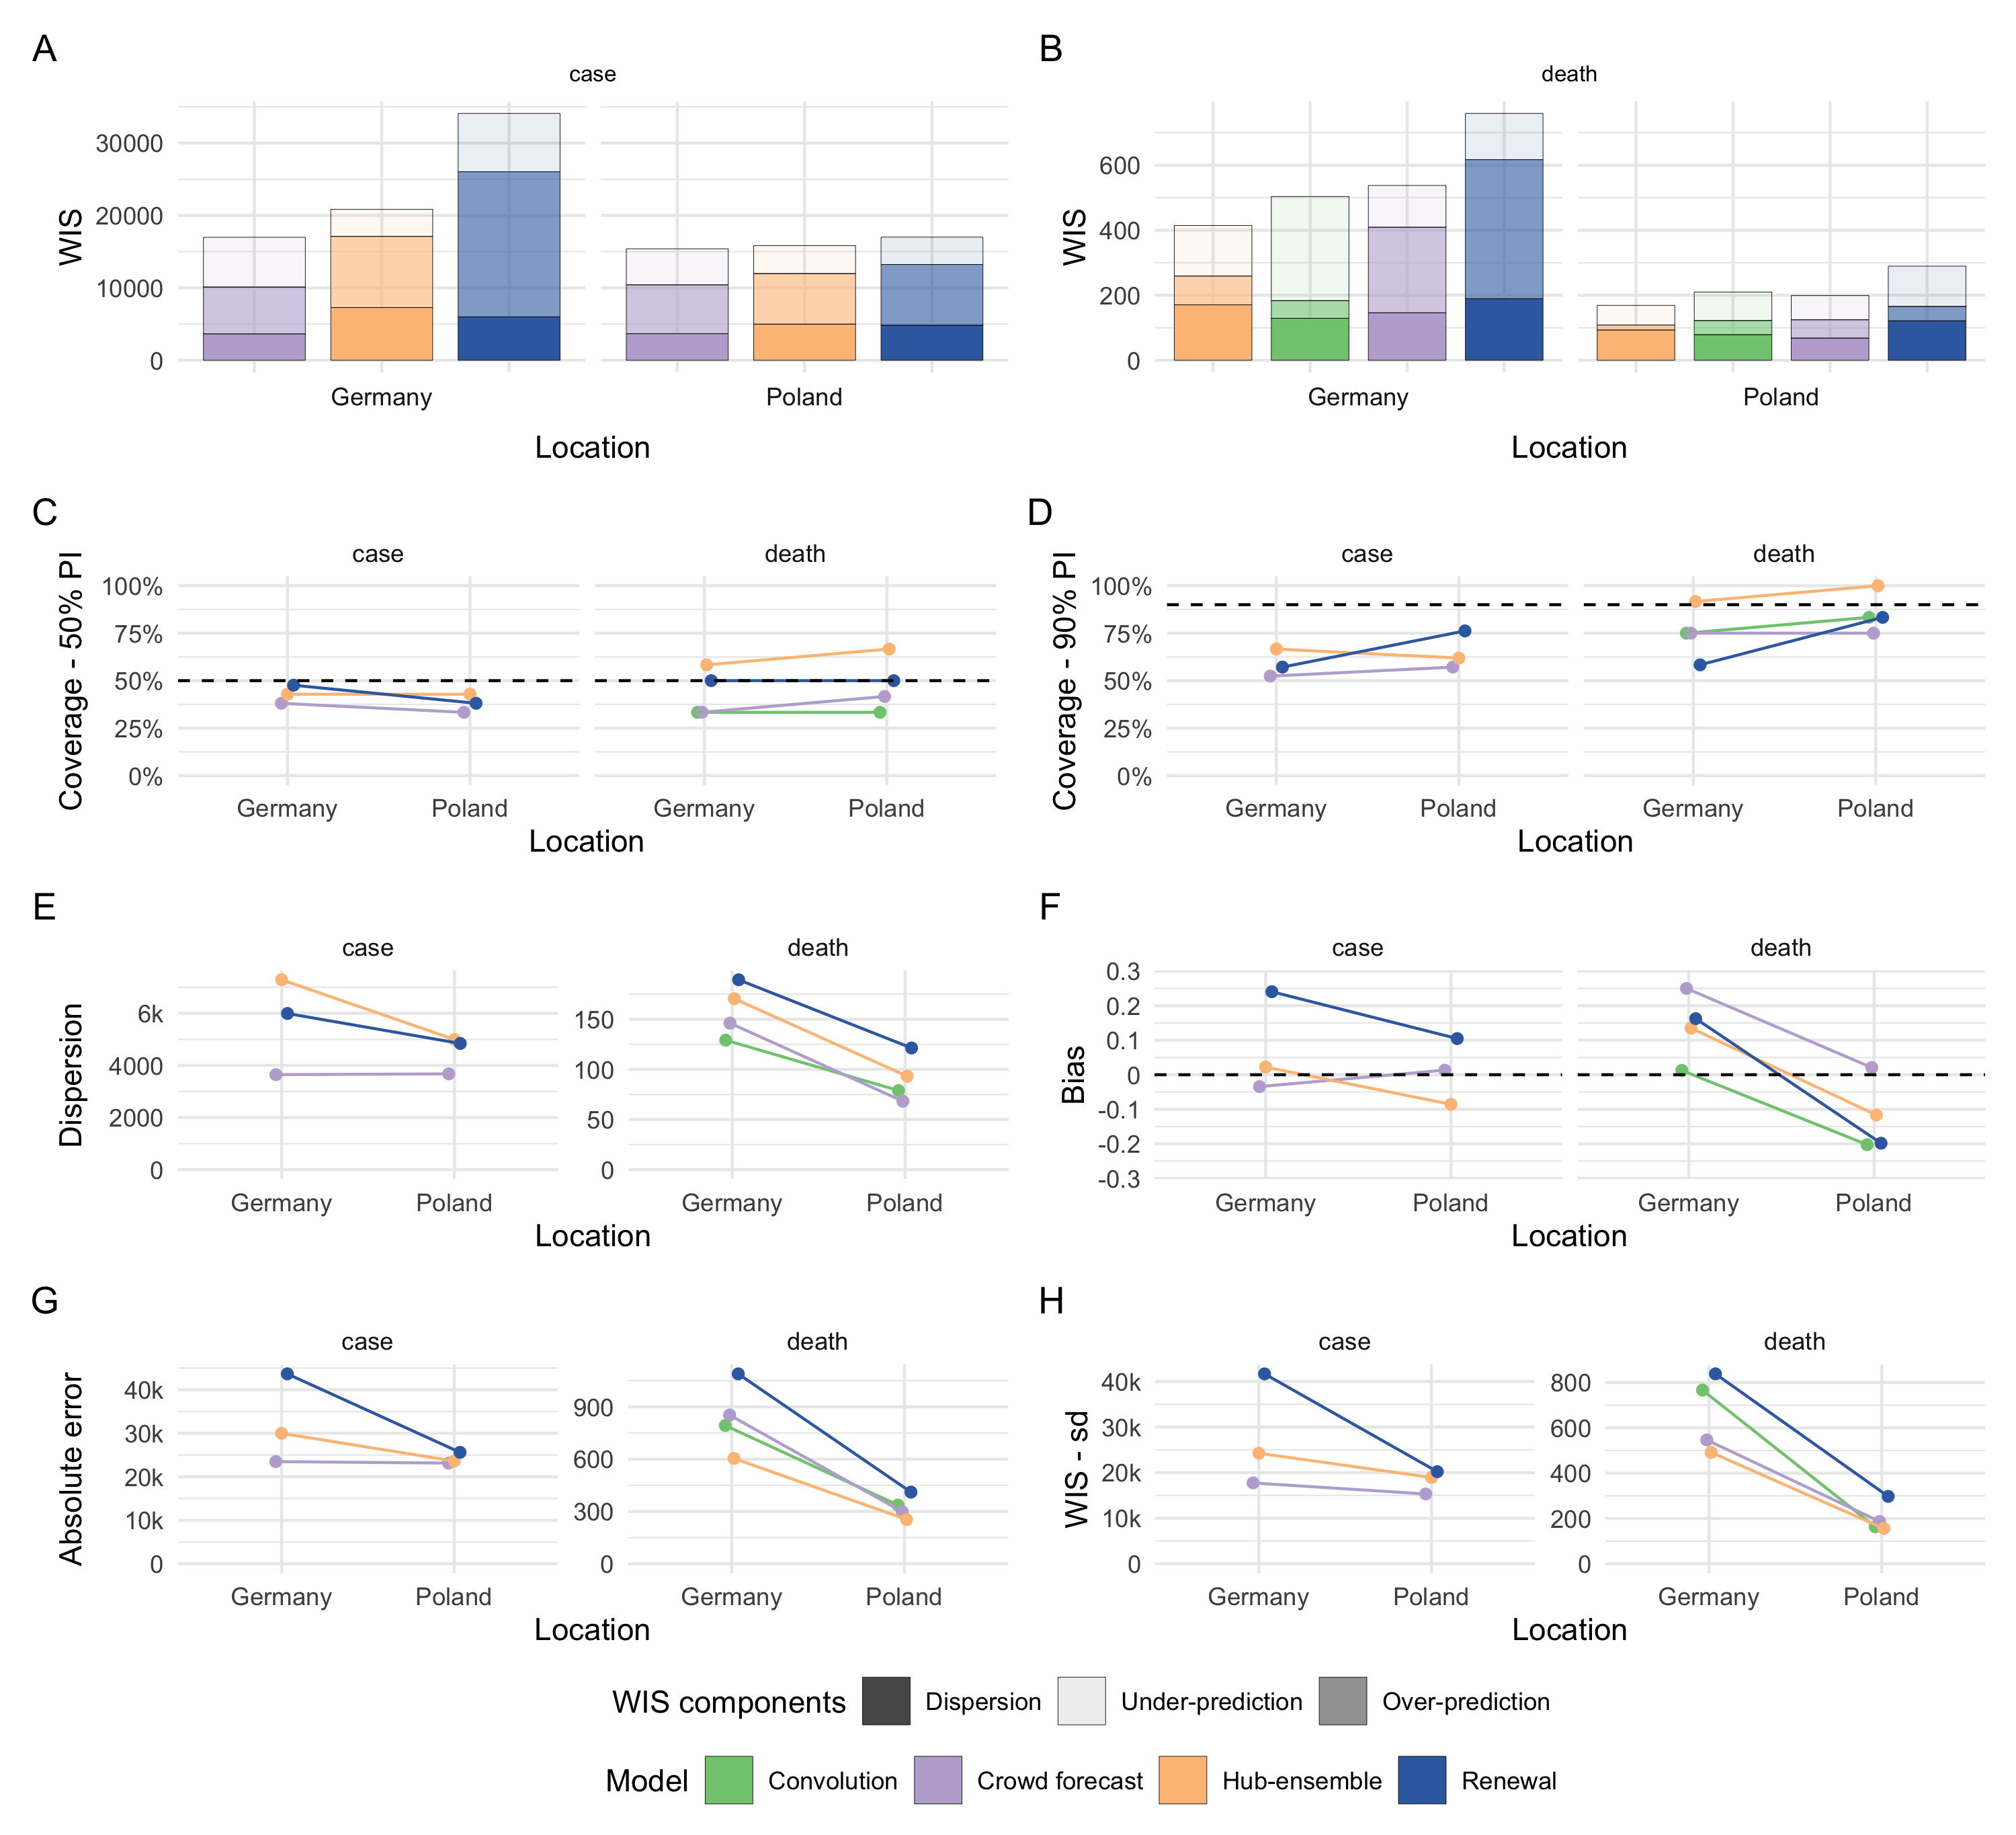
\includegraphics[width=1\linewidth,]{../analysis/plots/aggregate-performance-2-weeks-locations-all-v4} \caption{Visualisation of aggregate performance metrics across locations. A: mean weighted interval score (WIS) across horizons. B: median WIS. C: Absolute error of the median forecast. D: Standard deviation of the WIS. E: Dispersion (higher values mean further spread out forecast). F: Bias, i.e. general tendency to over- or underpredict. Values are between -1 (complete under-prediction) and 1 (complete over-prediction) and 0 ideally. G: Empirical coverage of the 50\% prediction intervals. F: Empirical coverage of the 90\% prediction intervals.}\label{fig:performance-locations}
\end{figure}

\hypertarget{performance-across-locations-in-relative-terms}{%
\subsection{Performance across locations in relative terms}\label{performance-across-locations-in-relative-terms}}

\begin{figure}[H]
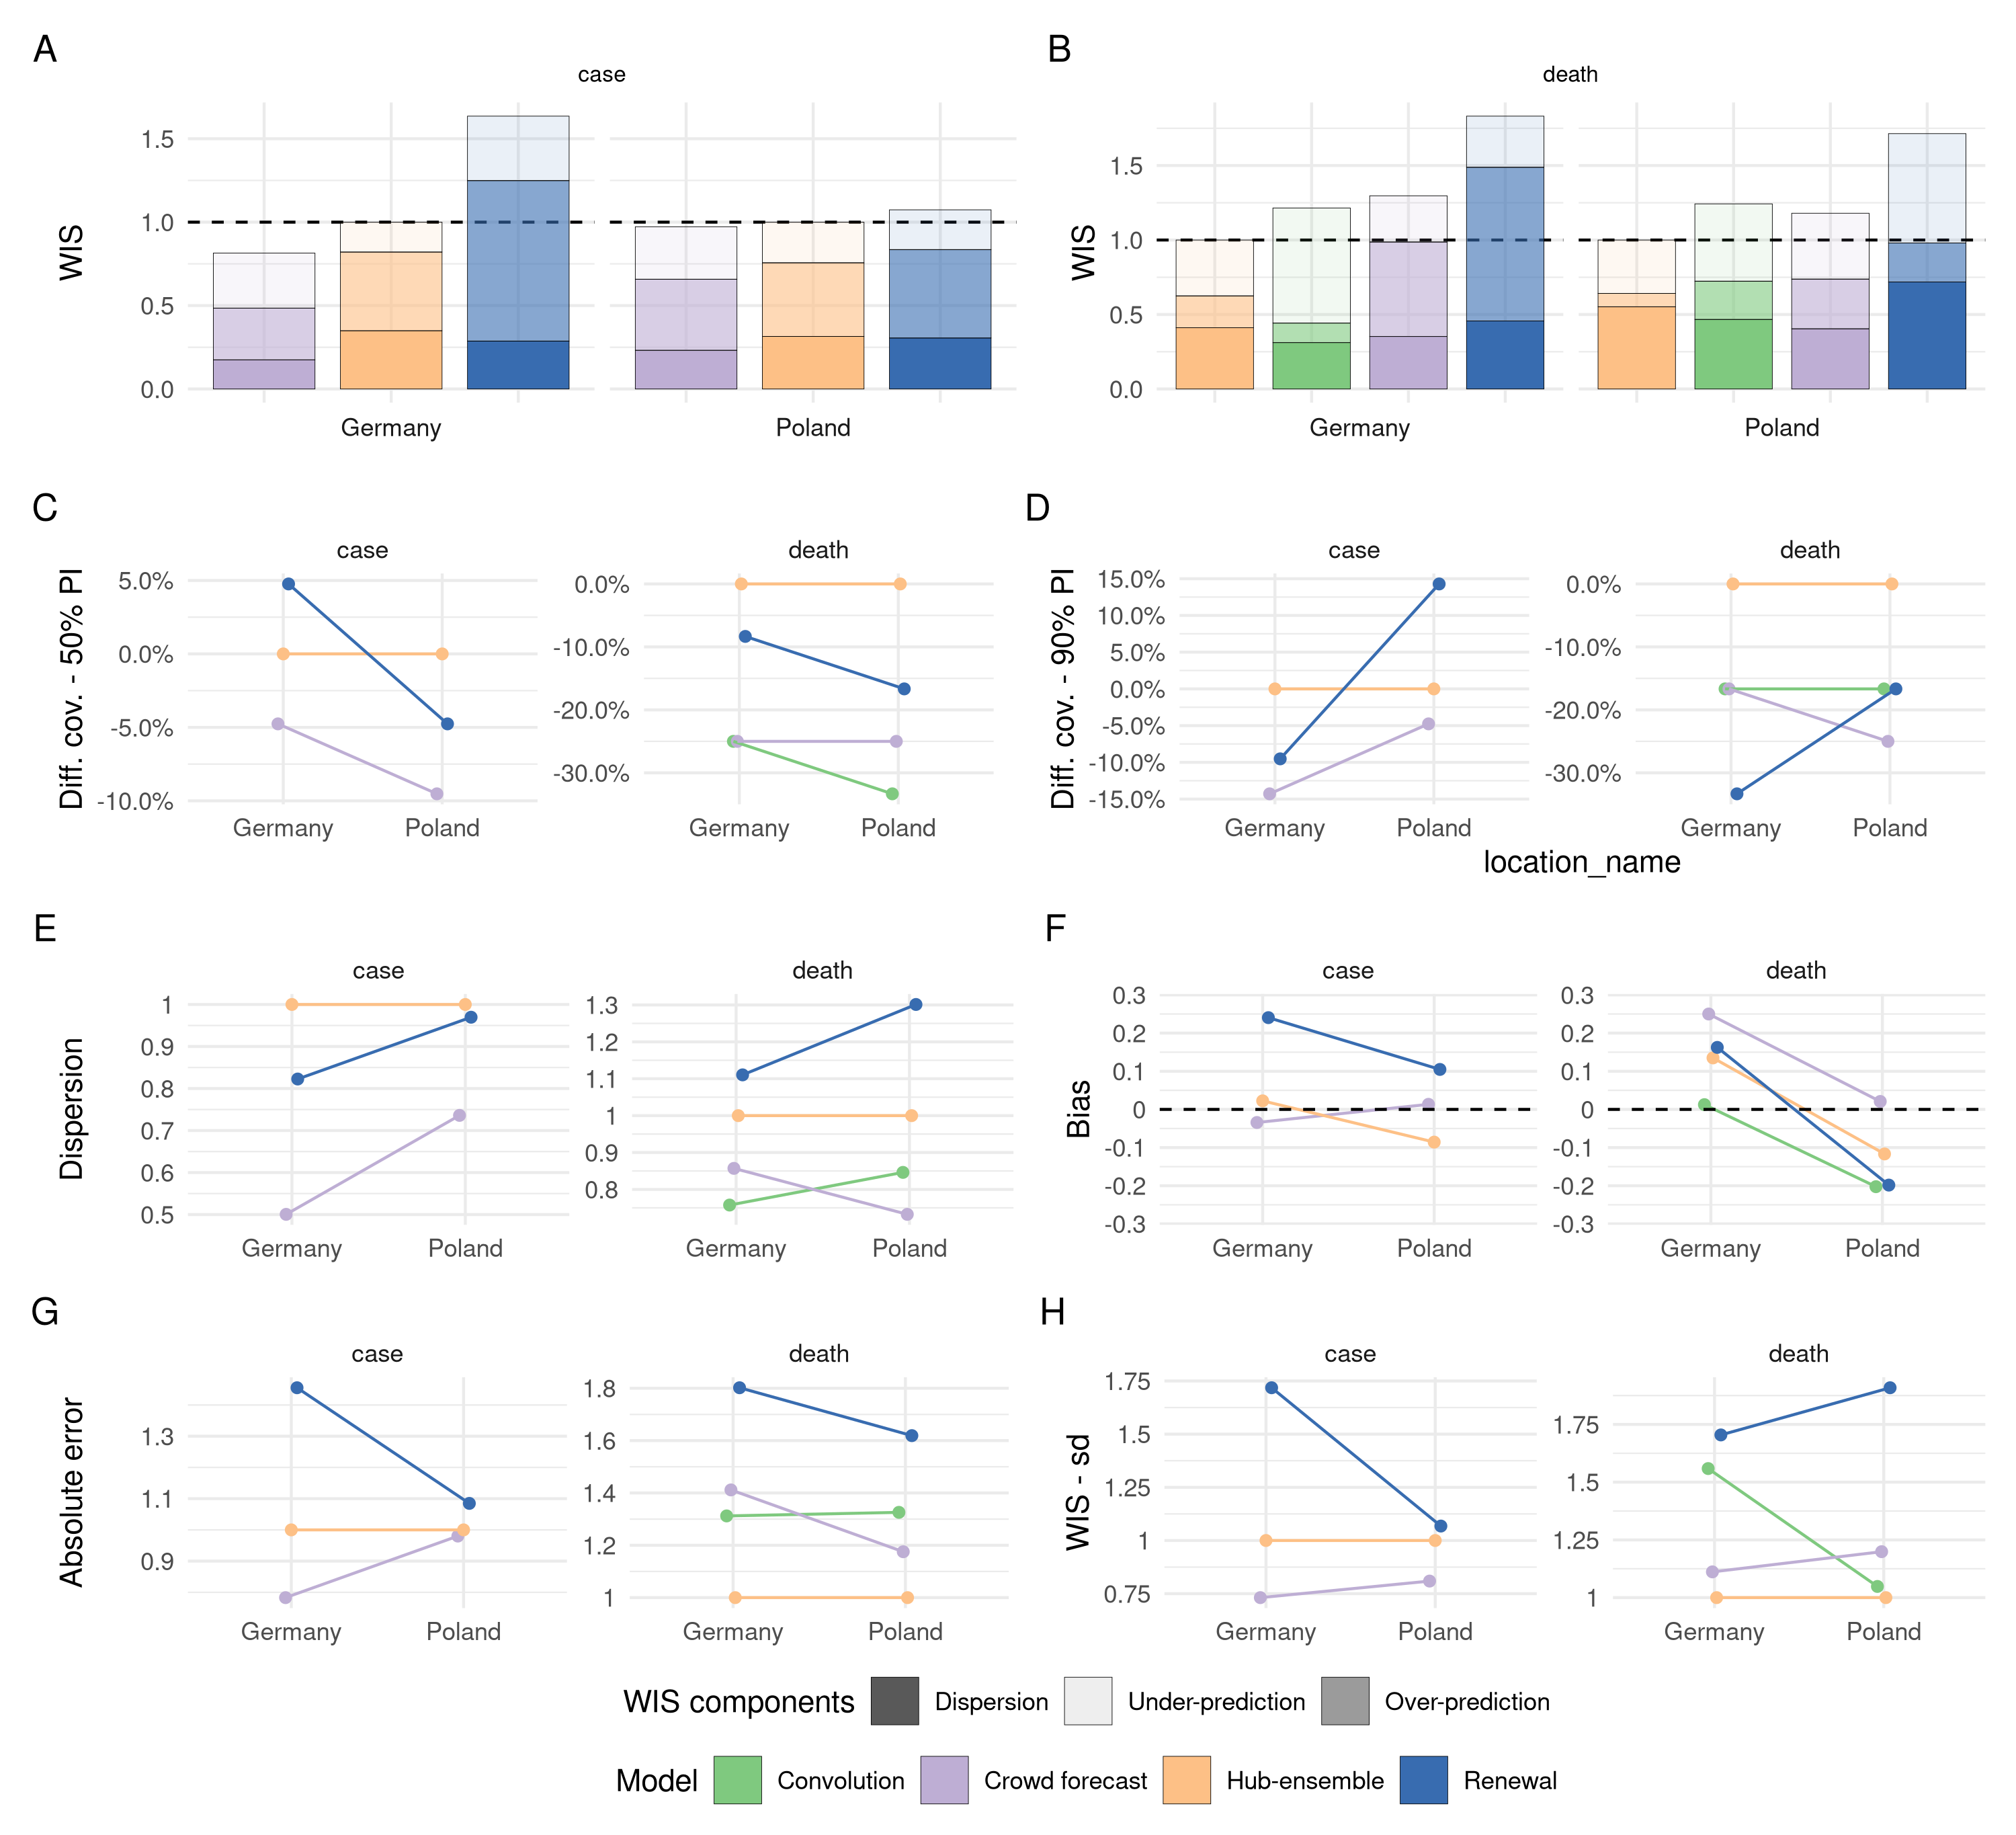
\includegraphics[width=1\linewidth,]{../analysis/plots/aggregate-performance-2-weeks-locations-all-rel-v4} \caption{ Visualisation of aggregate performance metrics across locations relative to the Hub ensemble (excluding our contributions). A: mean weighted interval score (WIS) across horizons. B: median WIS. C: Absolute error of the median forecast. D: Standard deviation of the WIS. E: Dispersion (higher values mean further spread out forecast). F: Bias, i.e. general tendency to over- or underpredict. Values are between -1 (complete under-prediction) and 1 (complete over-prediction) and 0 ideally. G: Empirical coverage of the 50\% prediction intervals. F: Empirical coverage of the 90\% prediction intervals.}\label{fig:performance-locations-rel}
\end{figure}

\clearpage

\hypertarget{visualisation-of-daily-reported-cases-and-deaths}{%
\subsection{Visualisation of daily reported cases and deaths}\label{visualisation-of-daily-reported-cases-and-deaths}}

\begin{figure}[H]
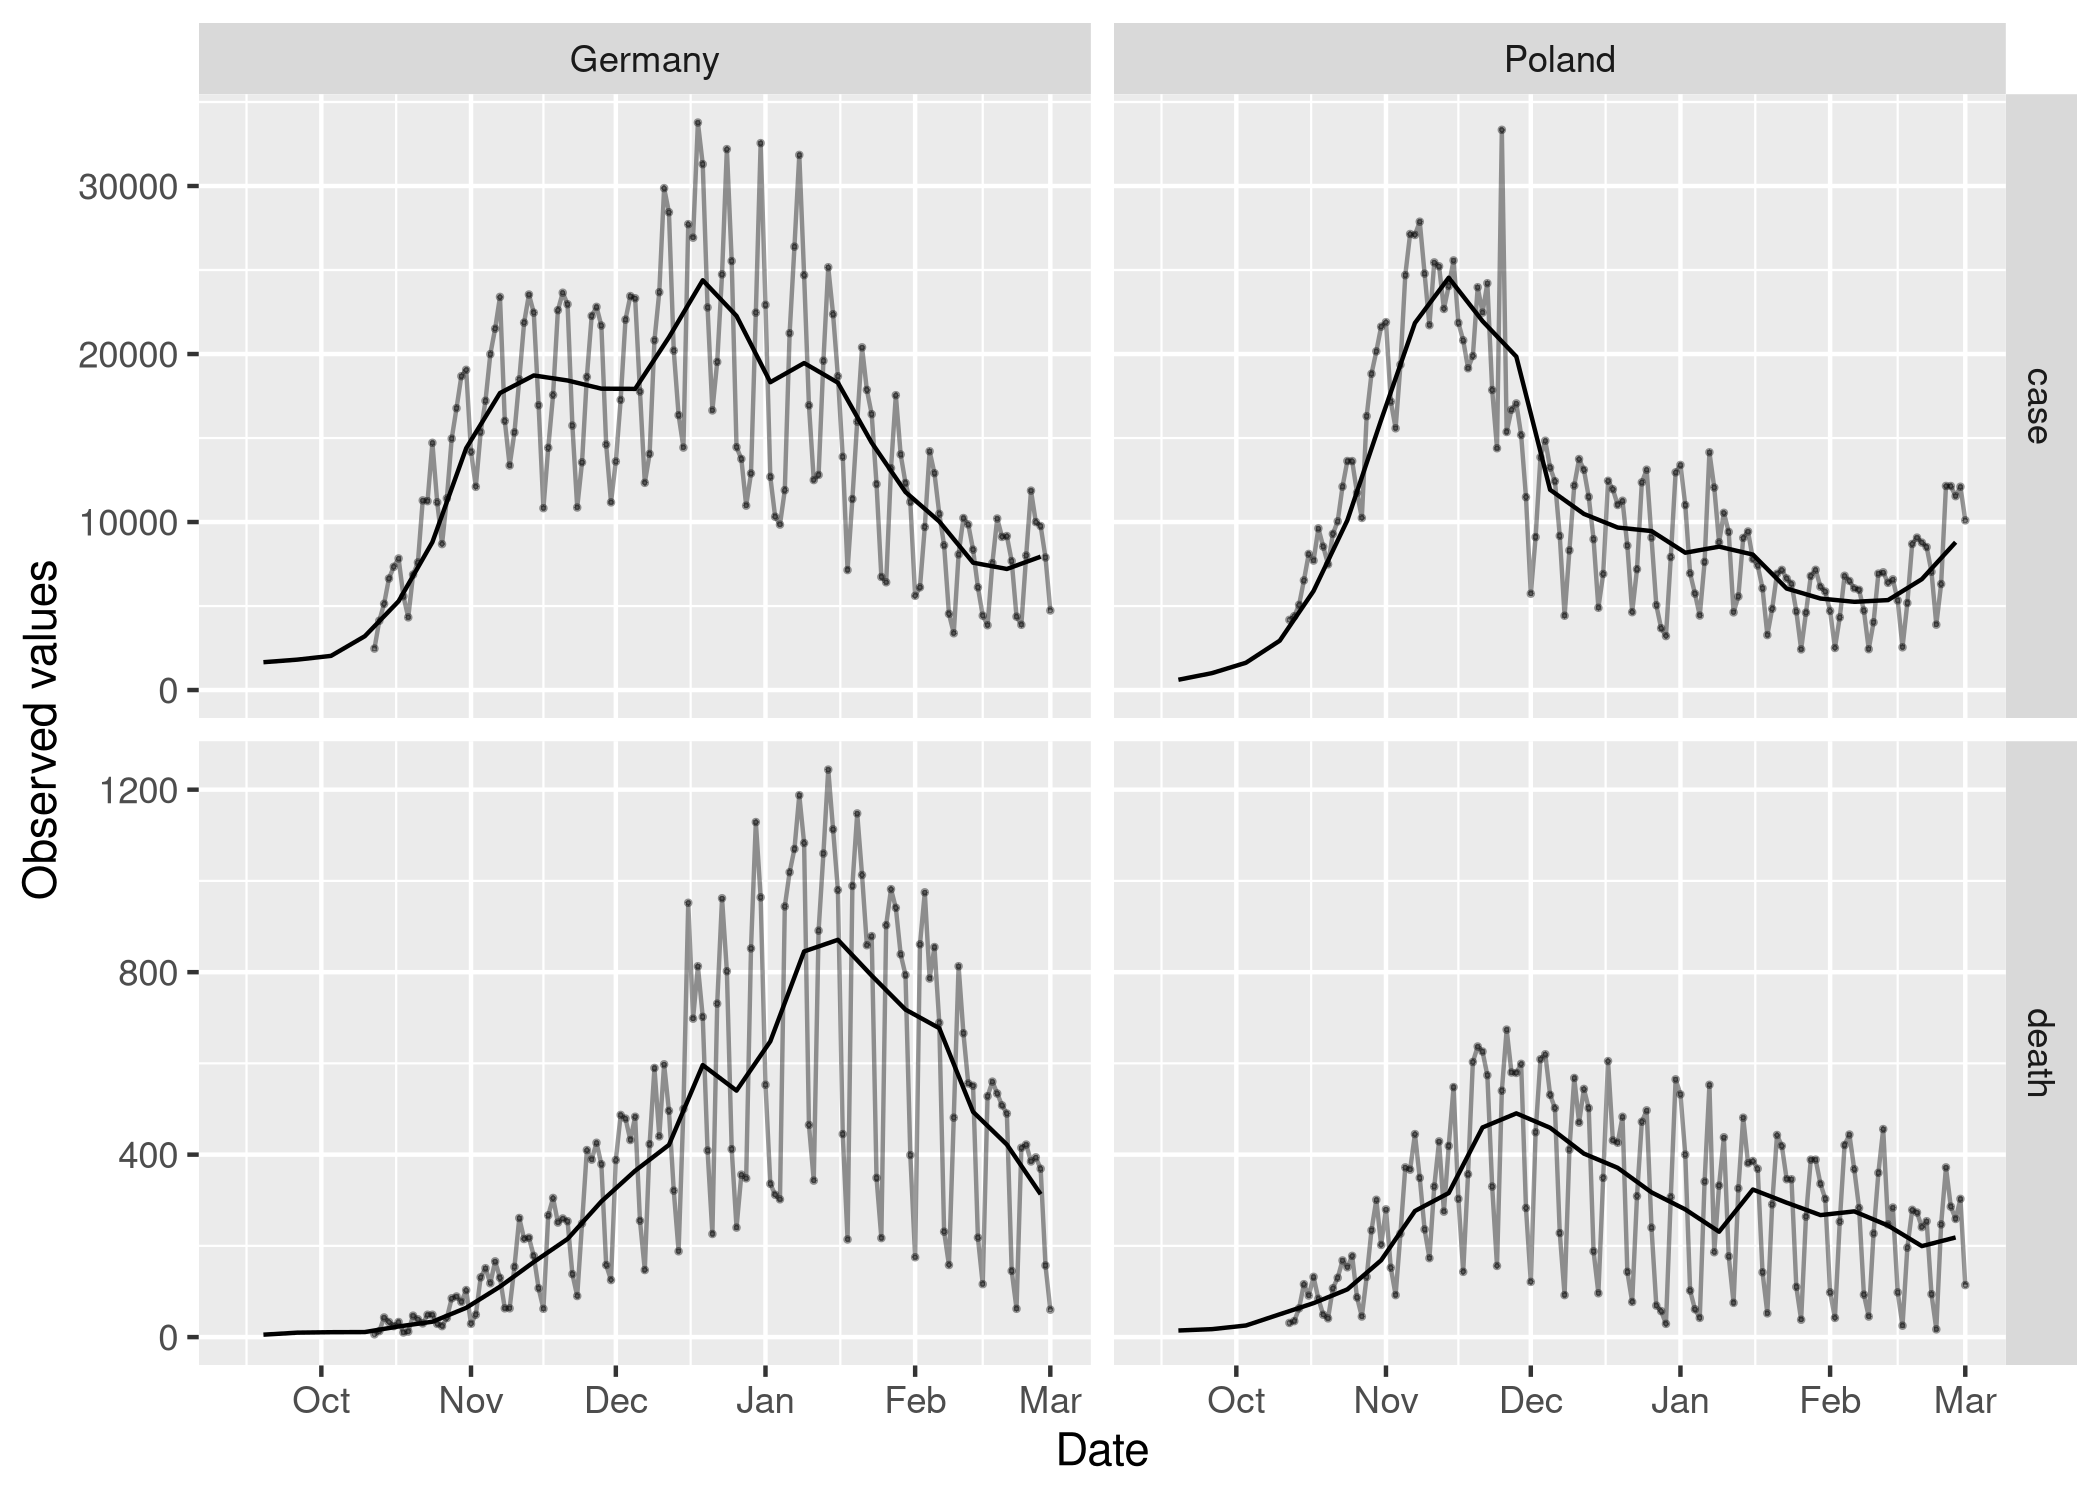
\includegraphics[width=1\linewidth,]{../analysis/plots/daily_truth} \caption{Visualisation of daily report data. The black line represents weekly data divided by seven. Data were last accessed through the German and Polish Forecast Hub on August 21 2021.}\label{fig:daily-truth}
\end{figure}

\clearpage

\hypertarget{visualisation-of-scores-and-forecasts-1-3-4-weeks-ahead}{%
\subsection{Visualisation of scores and forecasts 1, 3, 4 weeks ahead}\label{visualisation-of-scores-and-forecasts-1-3-4-weeks-ahead}}

\begin{figure}[H]
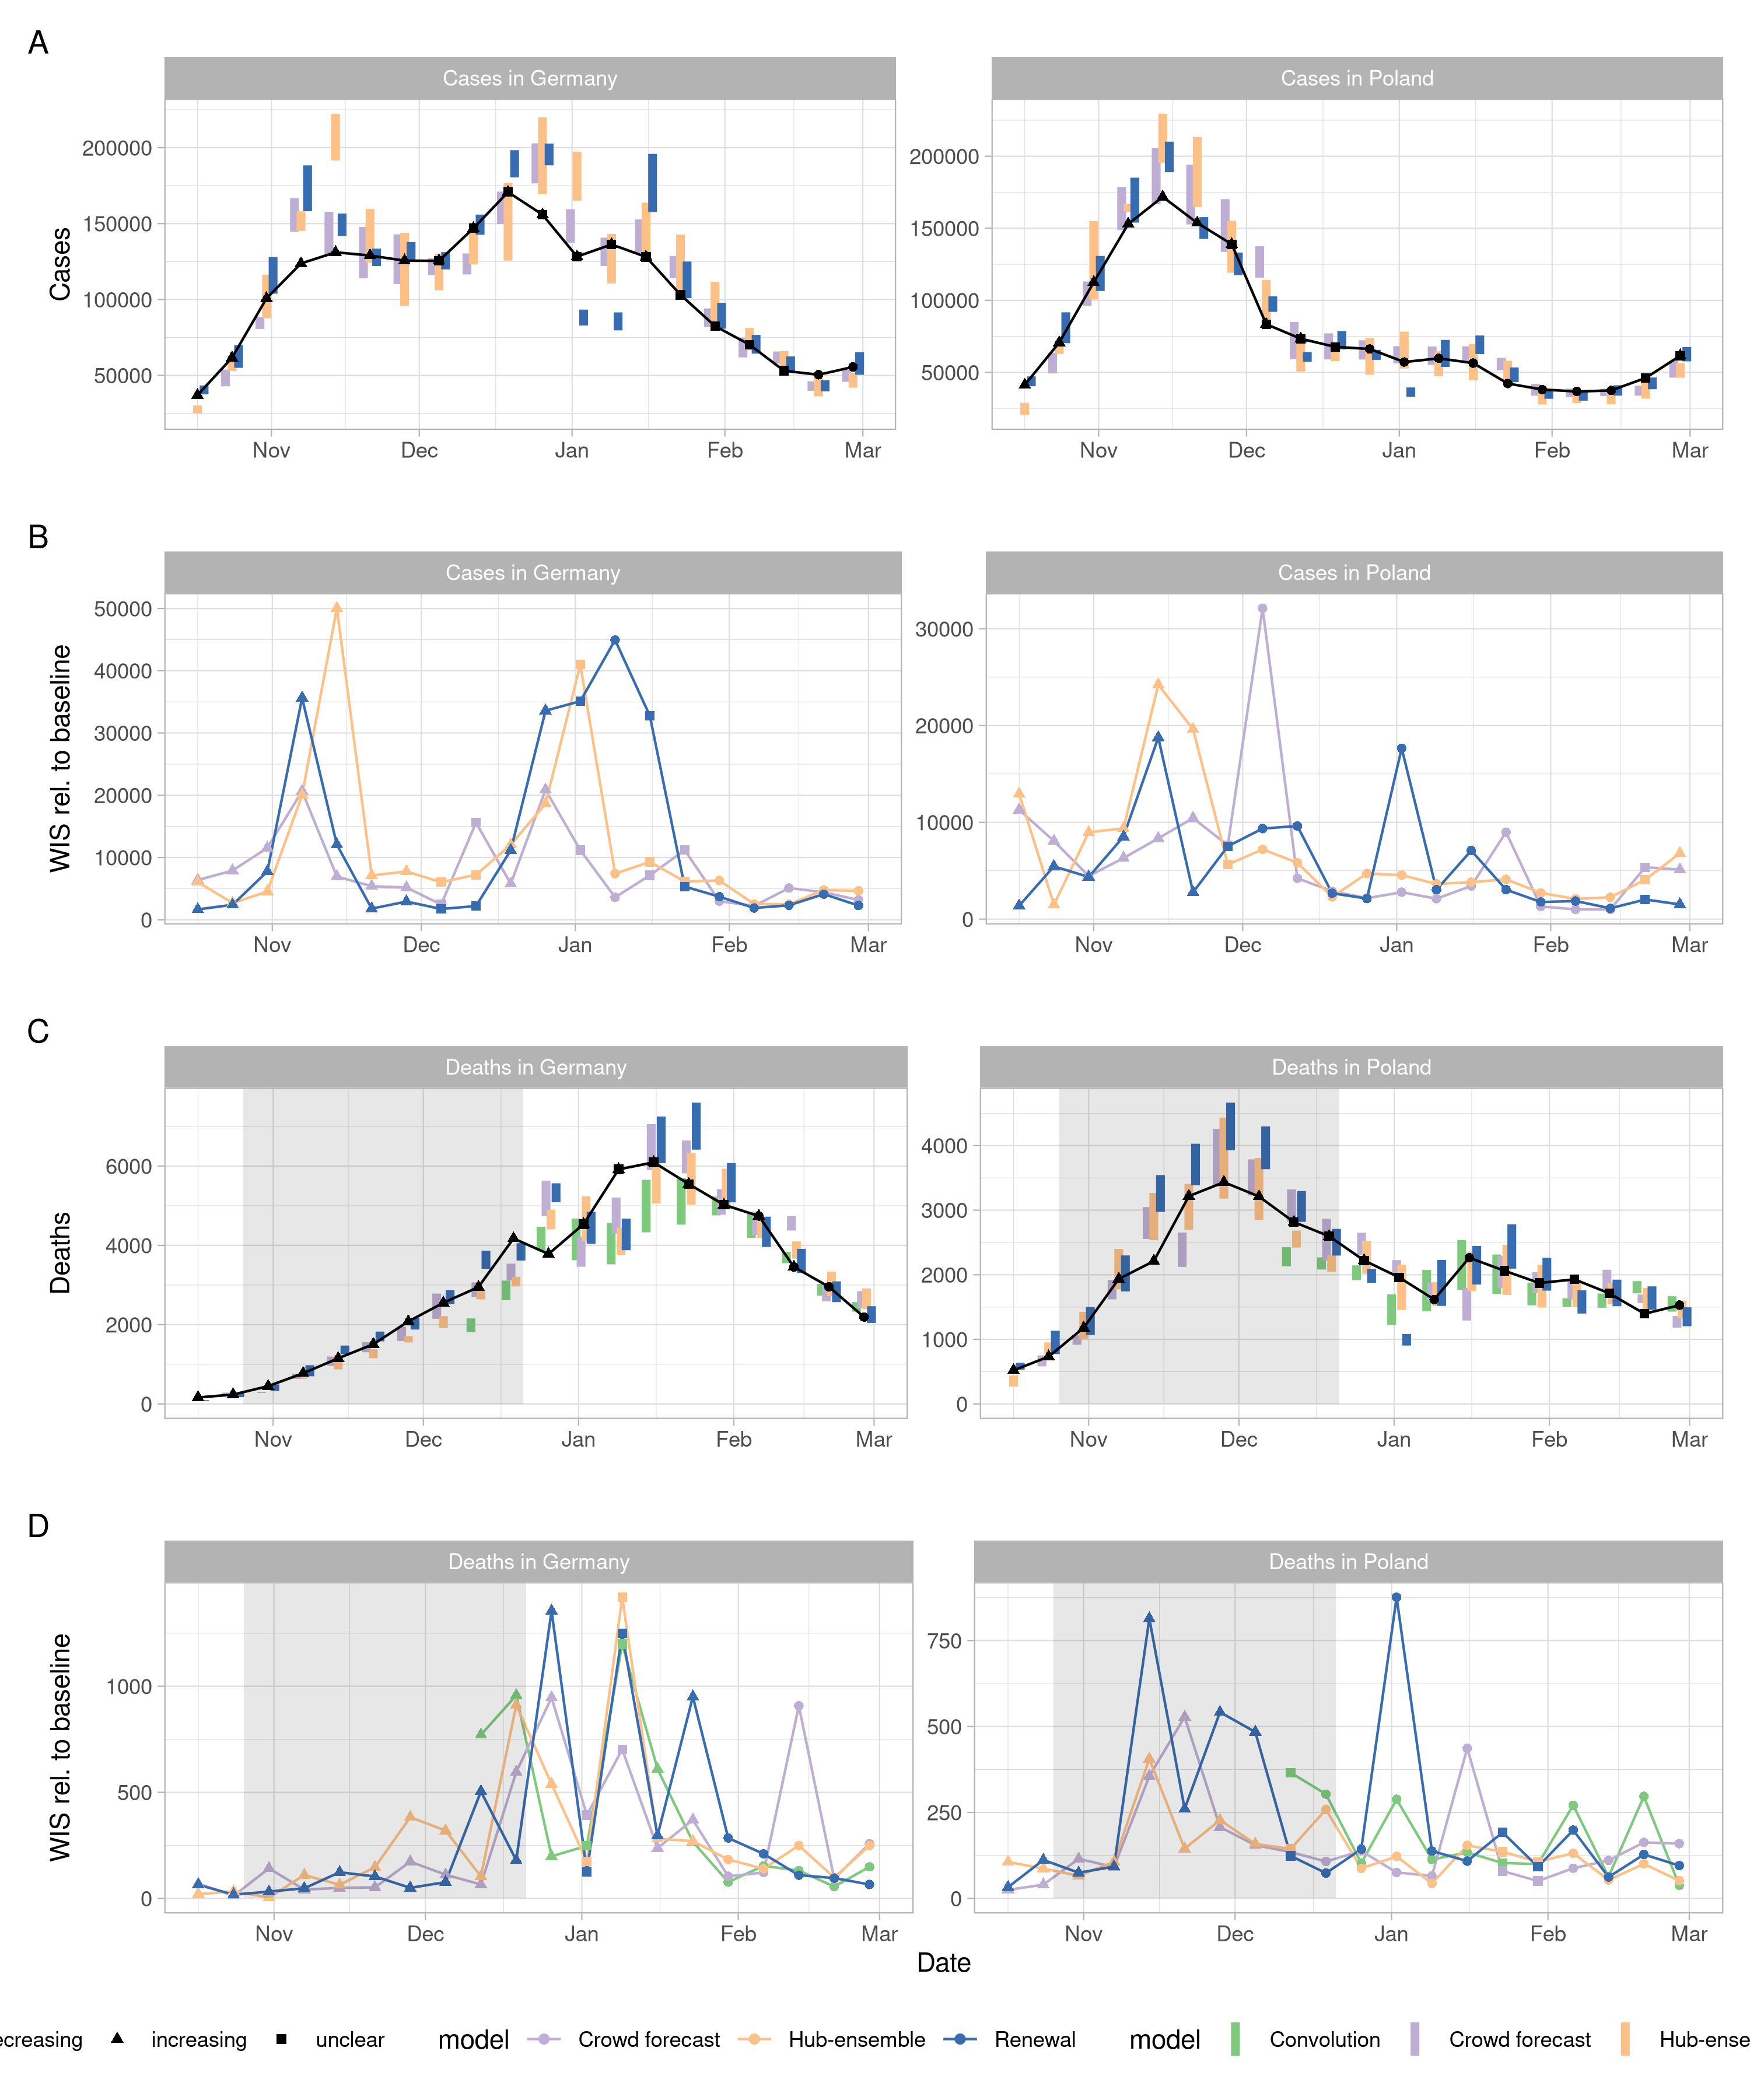
\includegraphics[width=1\linewidth,]{../analysis/plots/figure-forecasts-1} \caption{A, C: Visualisation of 50\% prediction intervals of one week ahead forecasts against the true observed values. Forecasts that were not scored (because there was no complete set of death forecasts available) are greyed out. B, D: Visualisation of corresponding WIS.}\label{fig:forecasts-and-truth-1}
\end{figure}

\begin{figure}[H]
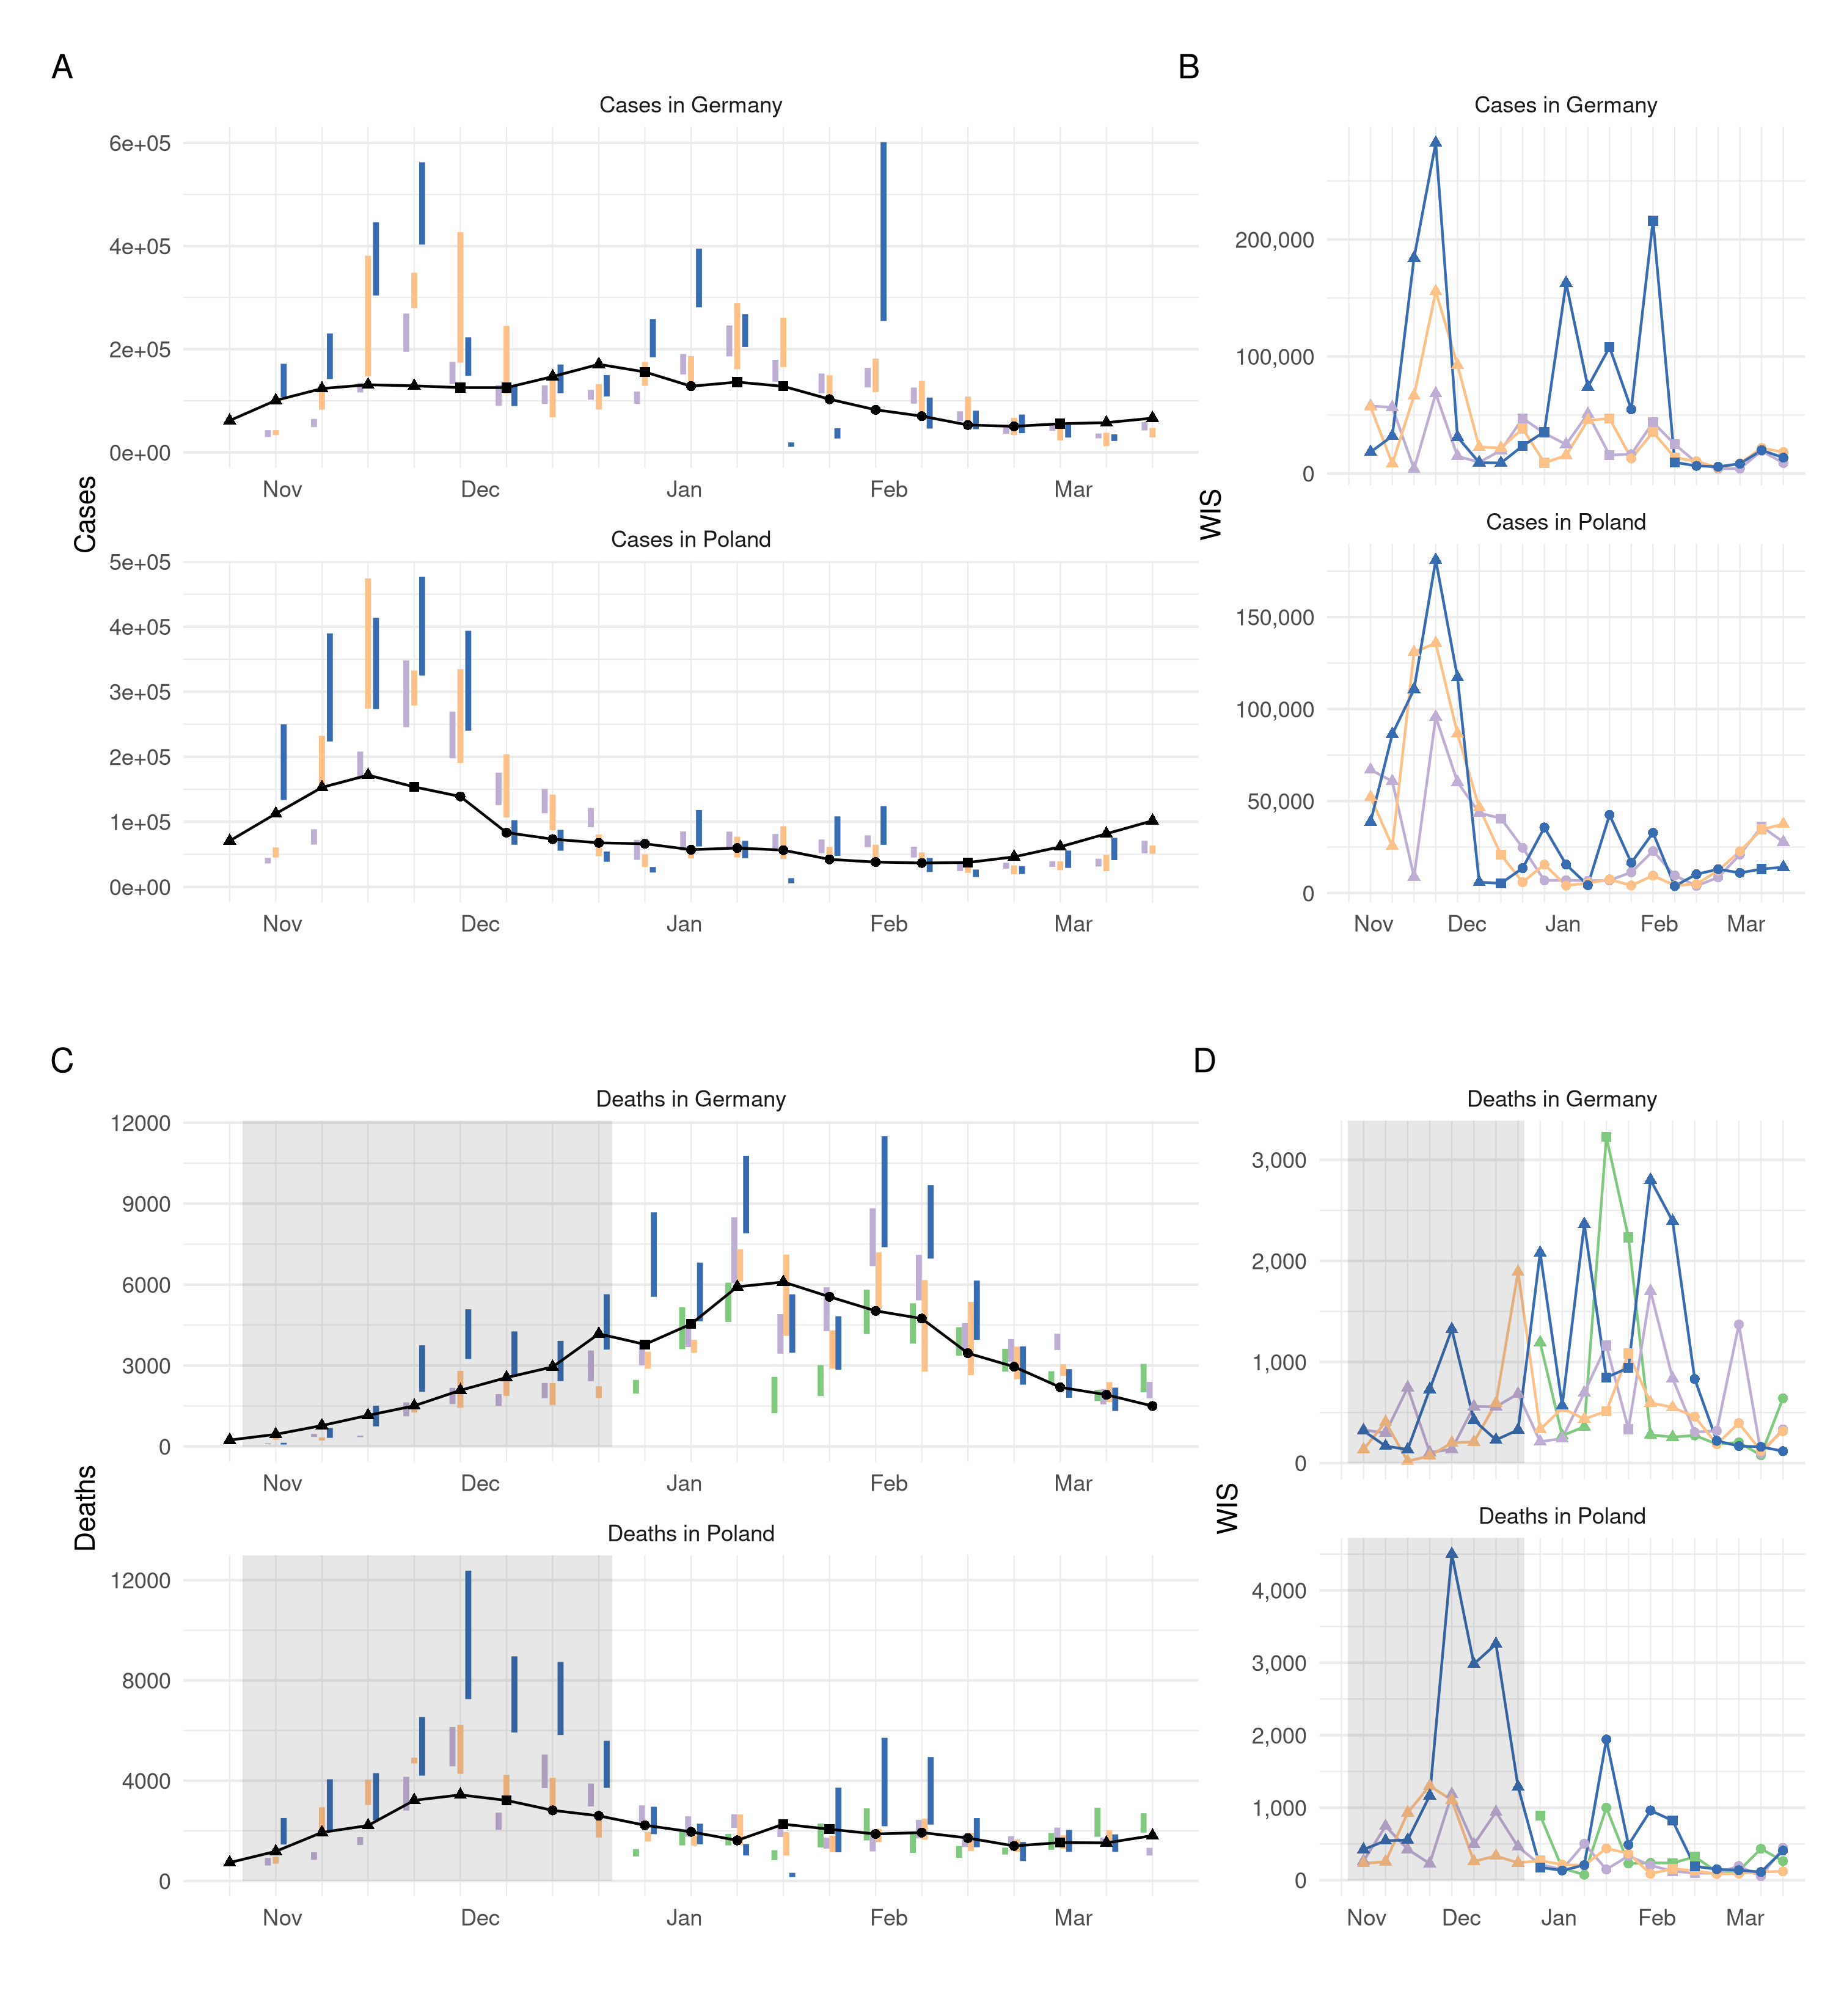
\includegraphics[width=1\linewidth,]{../analysis/plots/figure-forecasts-3} \caption{A, C: Visualisation of 50\% prediction intervals of three week ahead forecasts against the true observed values. Forecasts that were not scored (because there was no complete set of death forecasts available) are greyed out. B, D: Visualisation of corresponding WIS.}\label{fig:forecasts-and-truth-3}
\end{figure}

\begin{figure}[H]
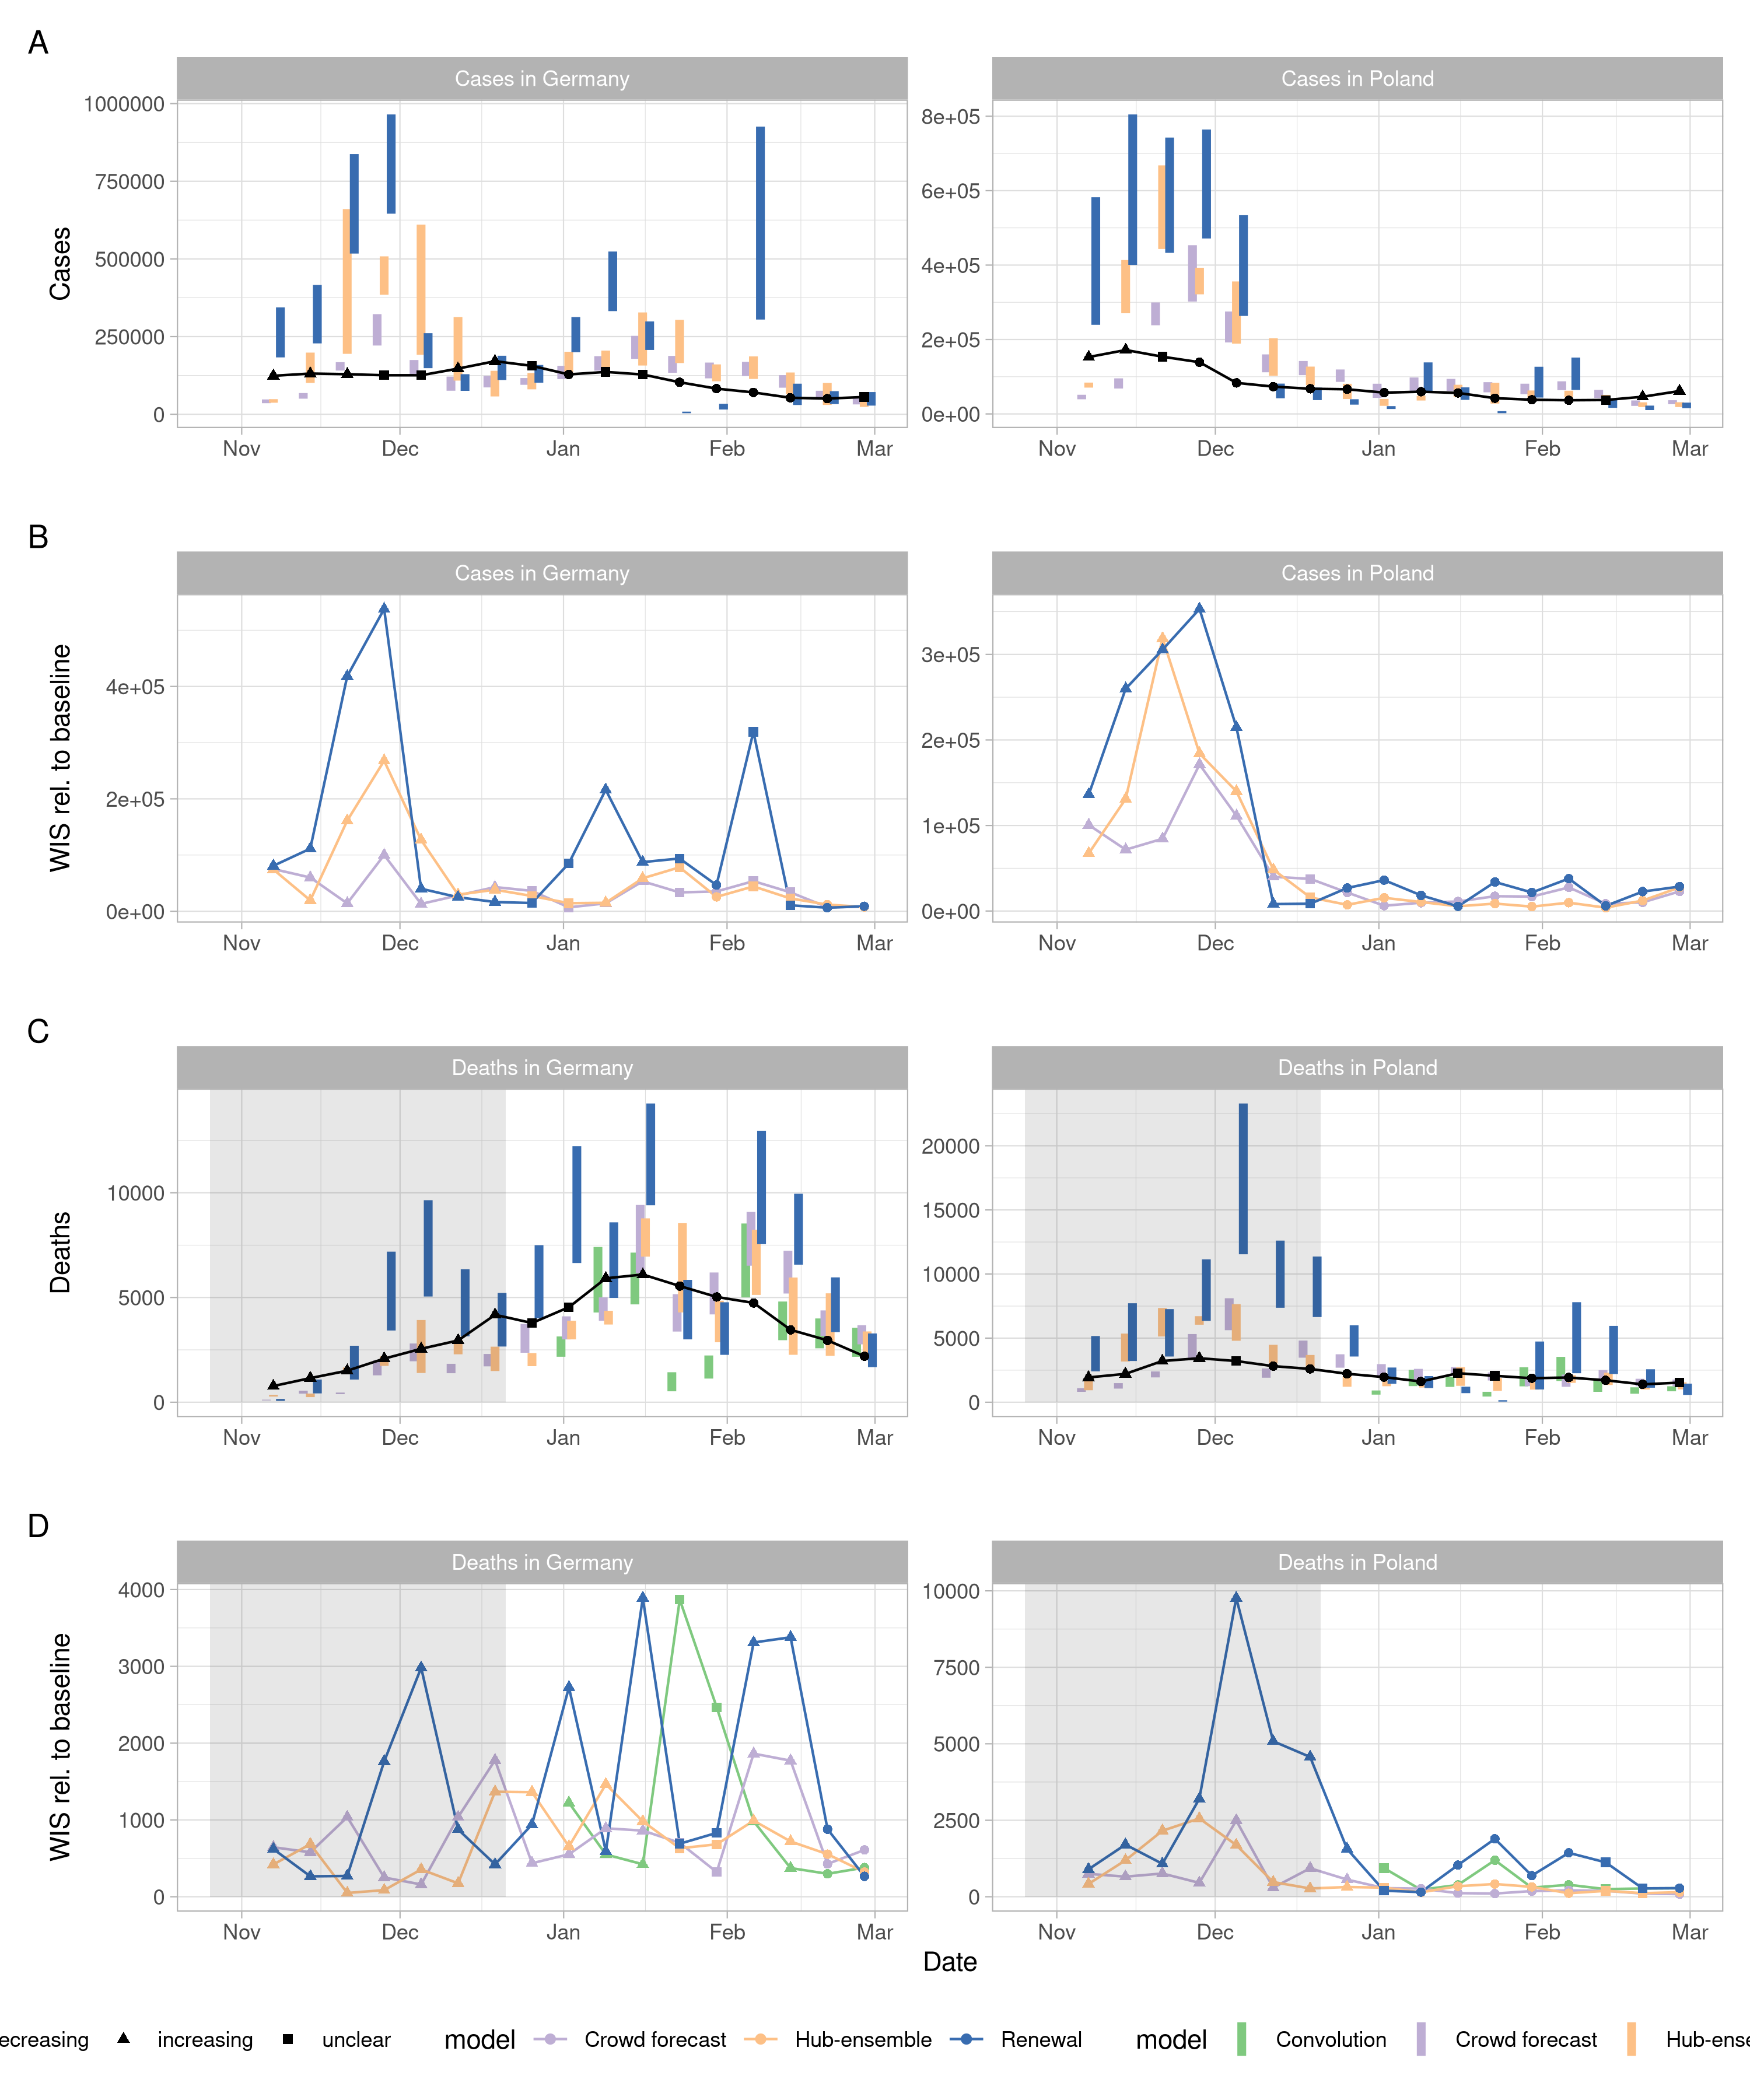
\includegraphics[width=1\linewidth,]{../analysis/plots/figure-forecasts-4} \caption{A, C: Visualisation of 50\% prediction intervals of four week ahead forecasts against the true observed values. Forecasts that were not scored (because there was no complete set of death forecasts available) are greyed out. B, D: Visualisation of corresponding WIS.}\label{fig:forecasts-and-truth-4}
\end{figure}

\clearpage

\hypertarget{distribution-of-scores}{%
\subsection{Distribution of scores}\label{distribution-of-scores}}

\hypertarget{absolute-scores}{%
\subsubsection{Absolute scores}\label{absolute-scores}}

\begin{figure}[H]
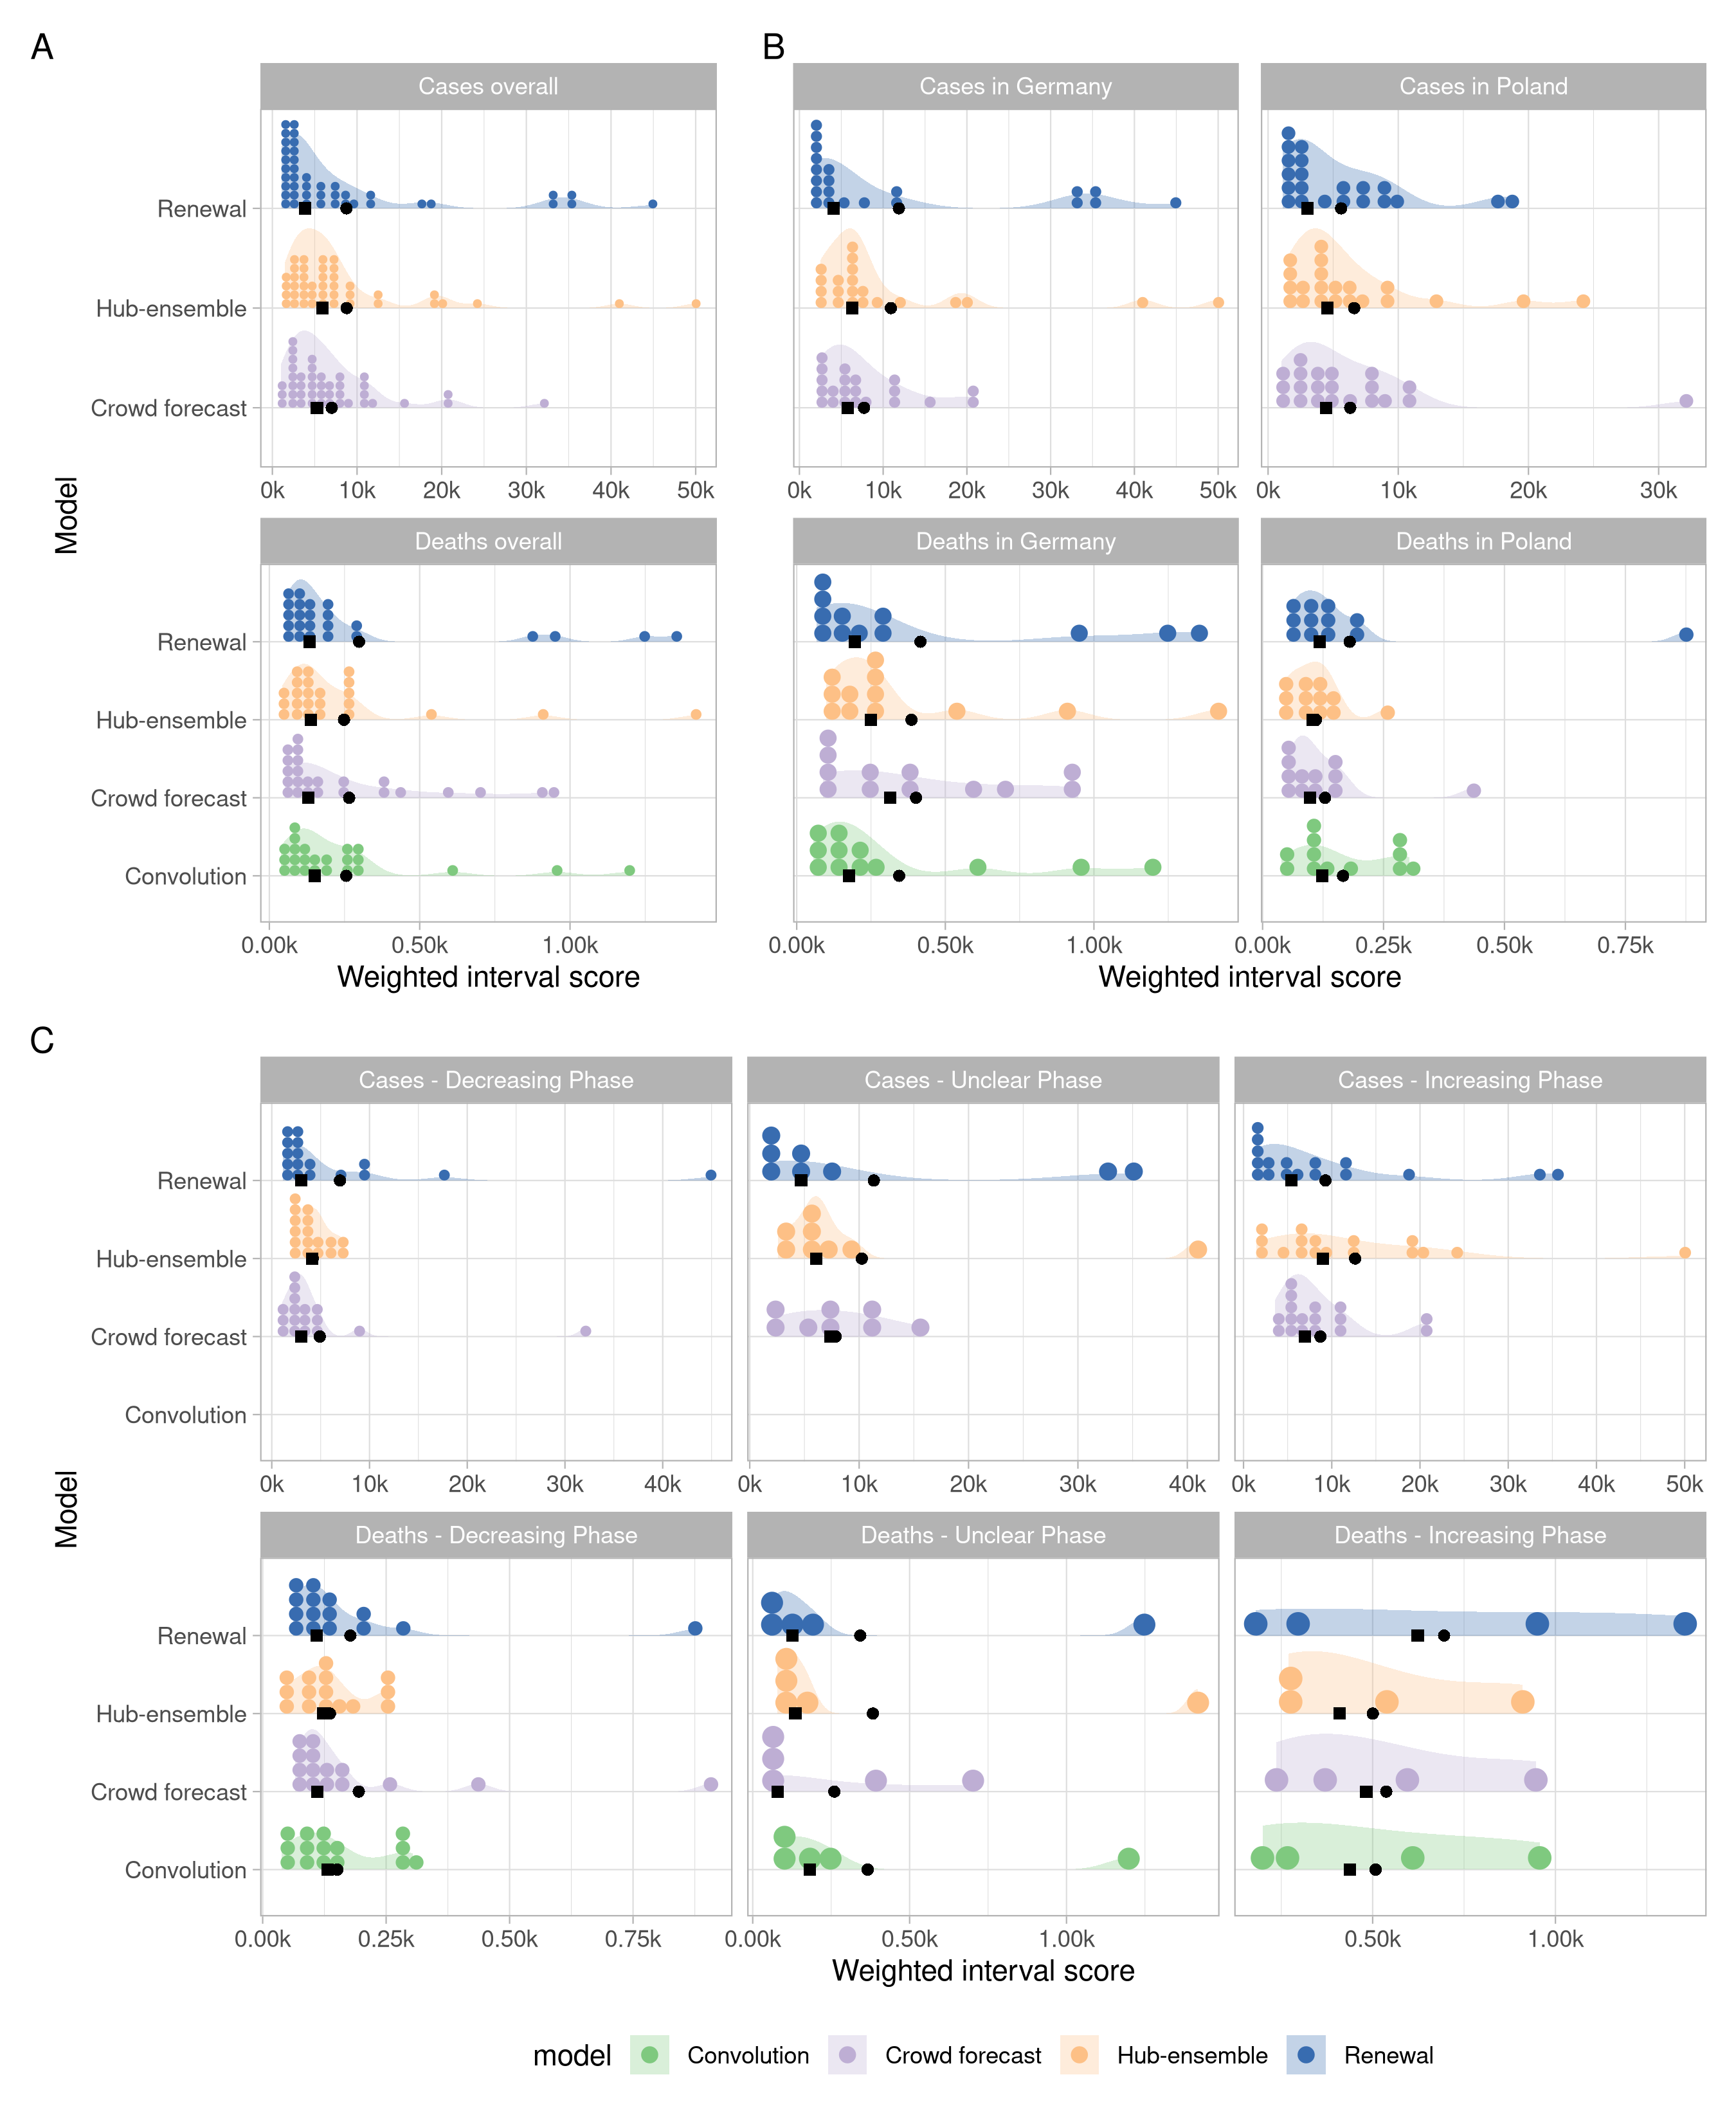
\includegraphics[width=1\linewidth,]{../analysis/plots/distribution_scores_wis-1} \caption{A: Distribution of weighted interval scores for one week ahead forecasts of the different models and forecast targets. B: Distribution of WIS separate by country.}\label{fig:distribution-scores-1}
\end{figure}

\begin{figure}[H]
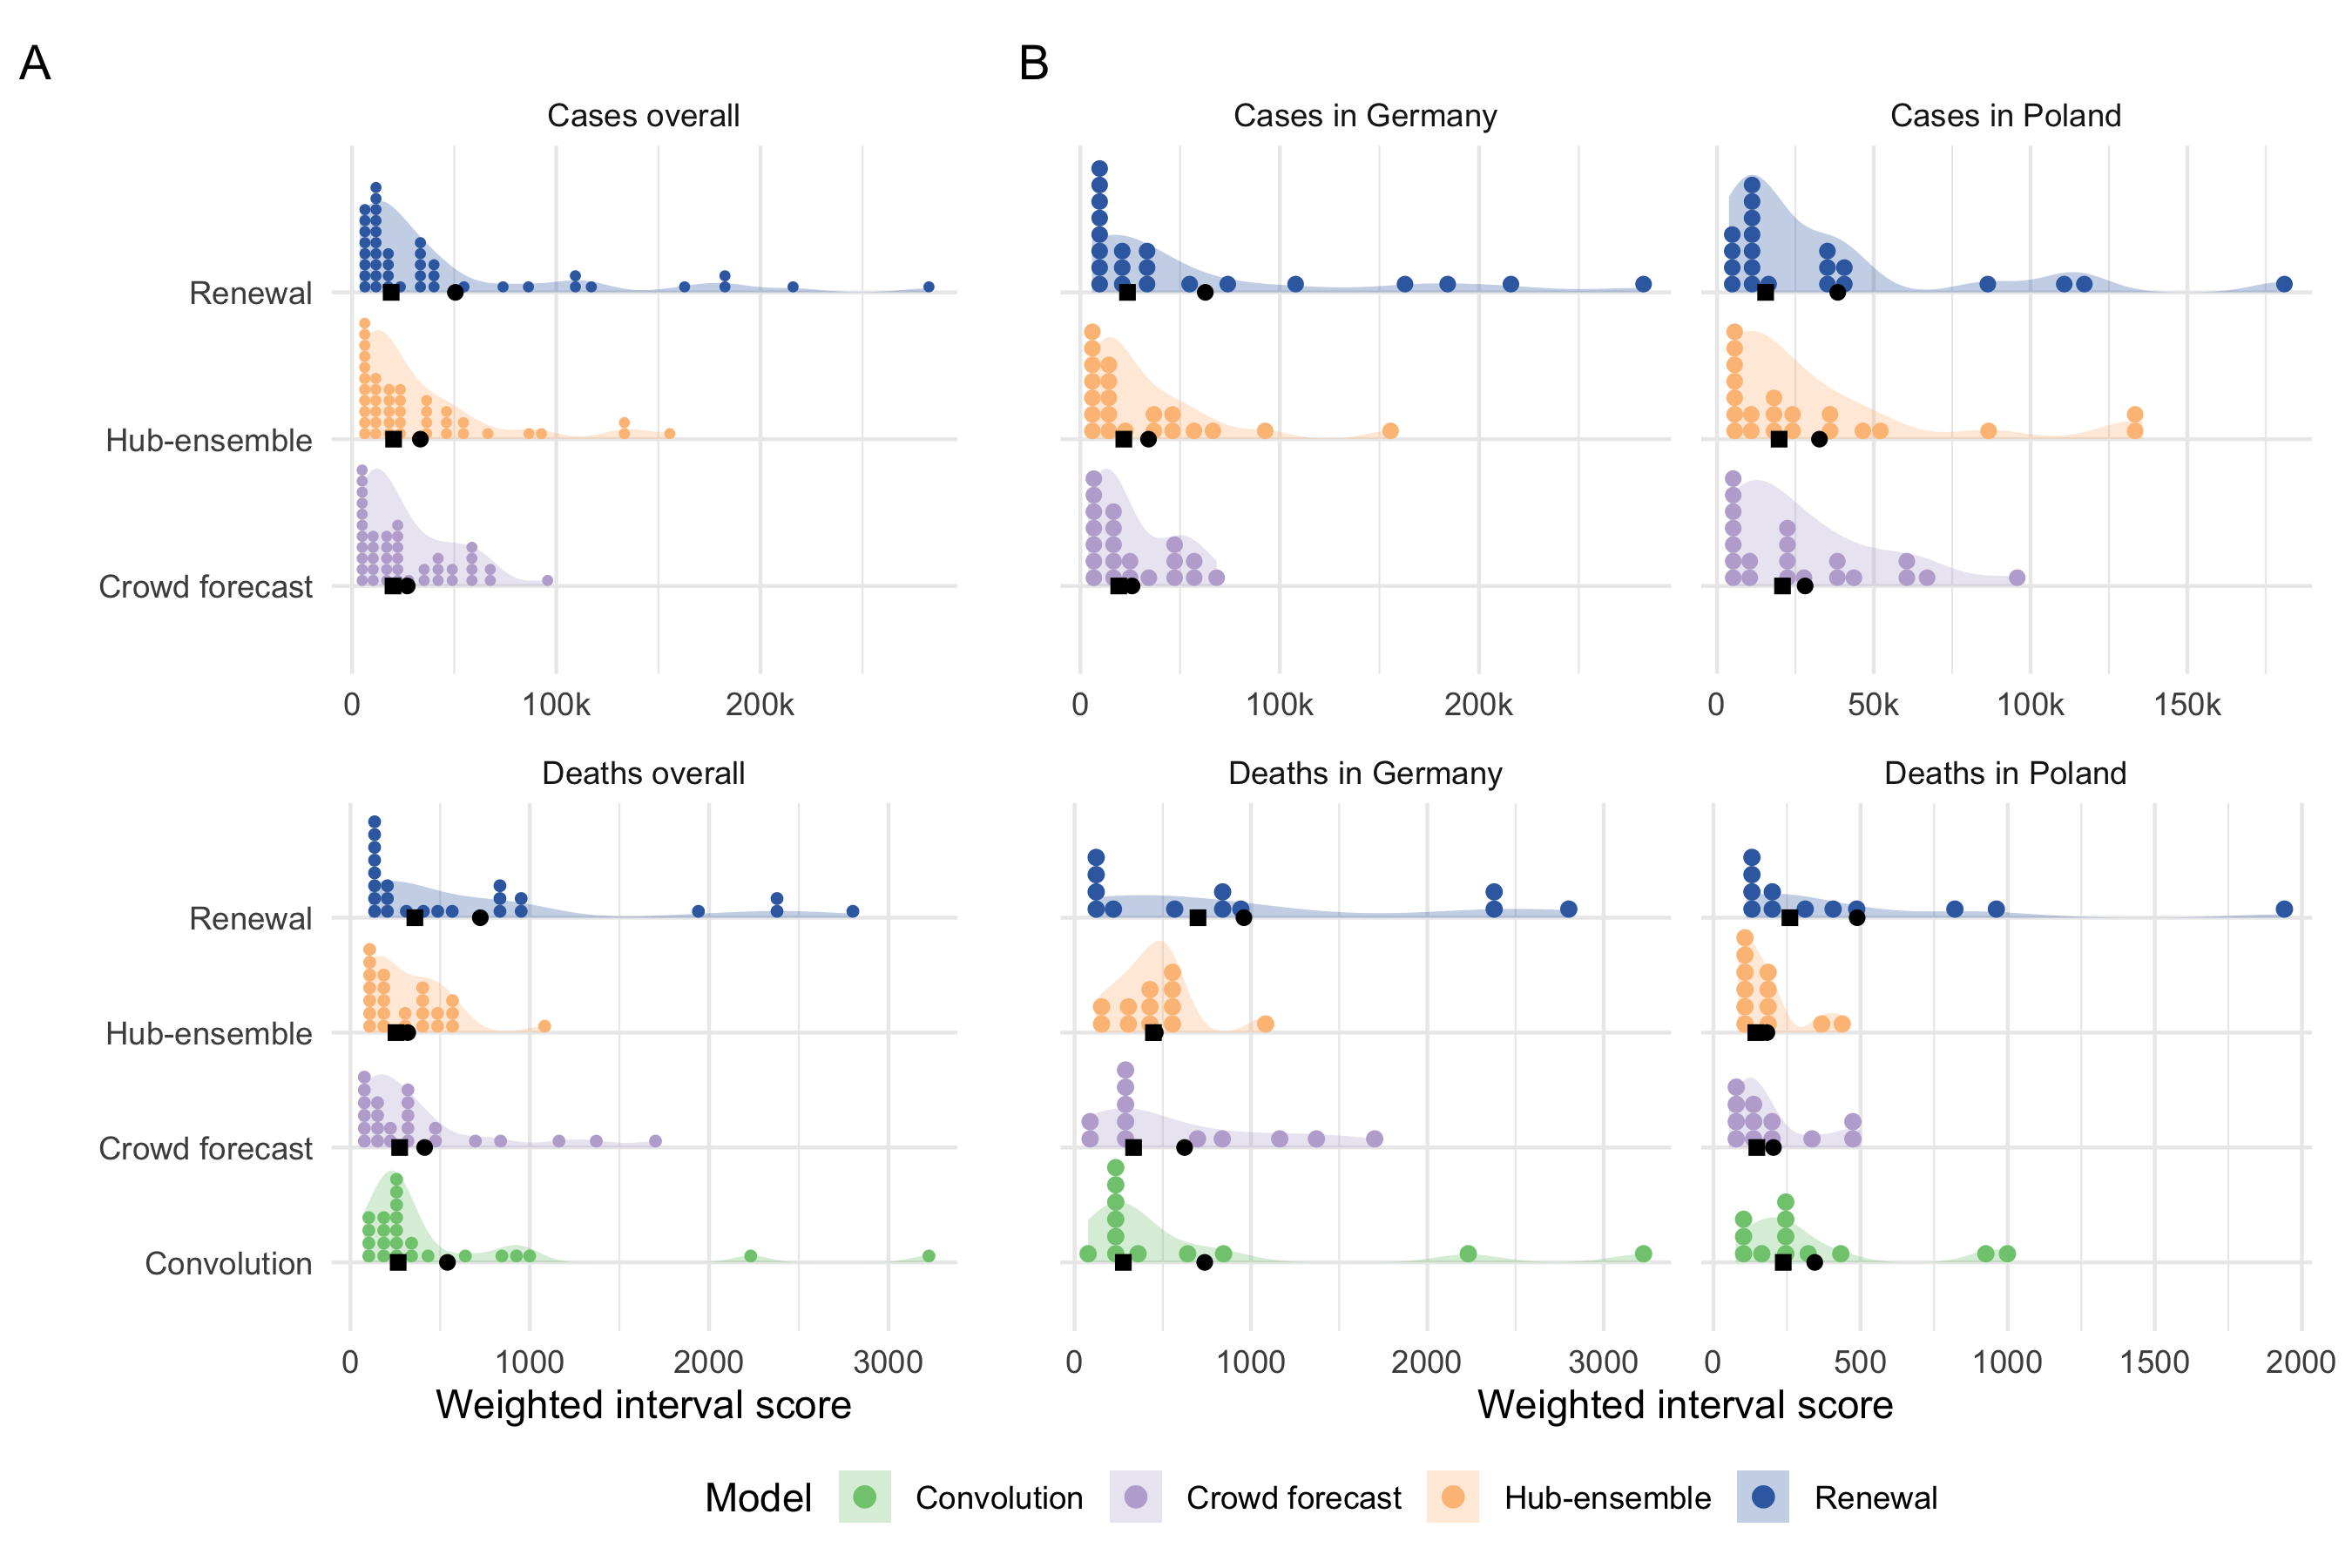
\includegraphics[width=1\linewidth,]{../analysis/plots/distribution_scores_wis-3} \caption{A: Distribution of weighted interval scores for three week ahead forecasts of the different models and forecast targets. B: Distribution of WIS separate by country.}\label{fig:distribution-scores-3}
\end{figure}

\begin{figure}[H]
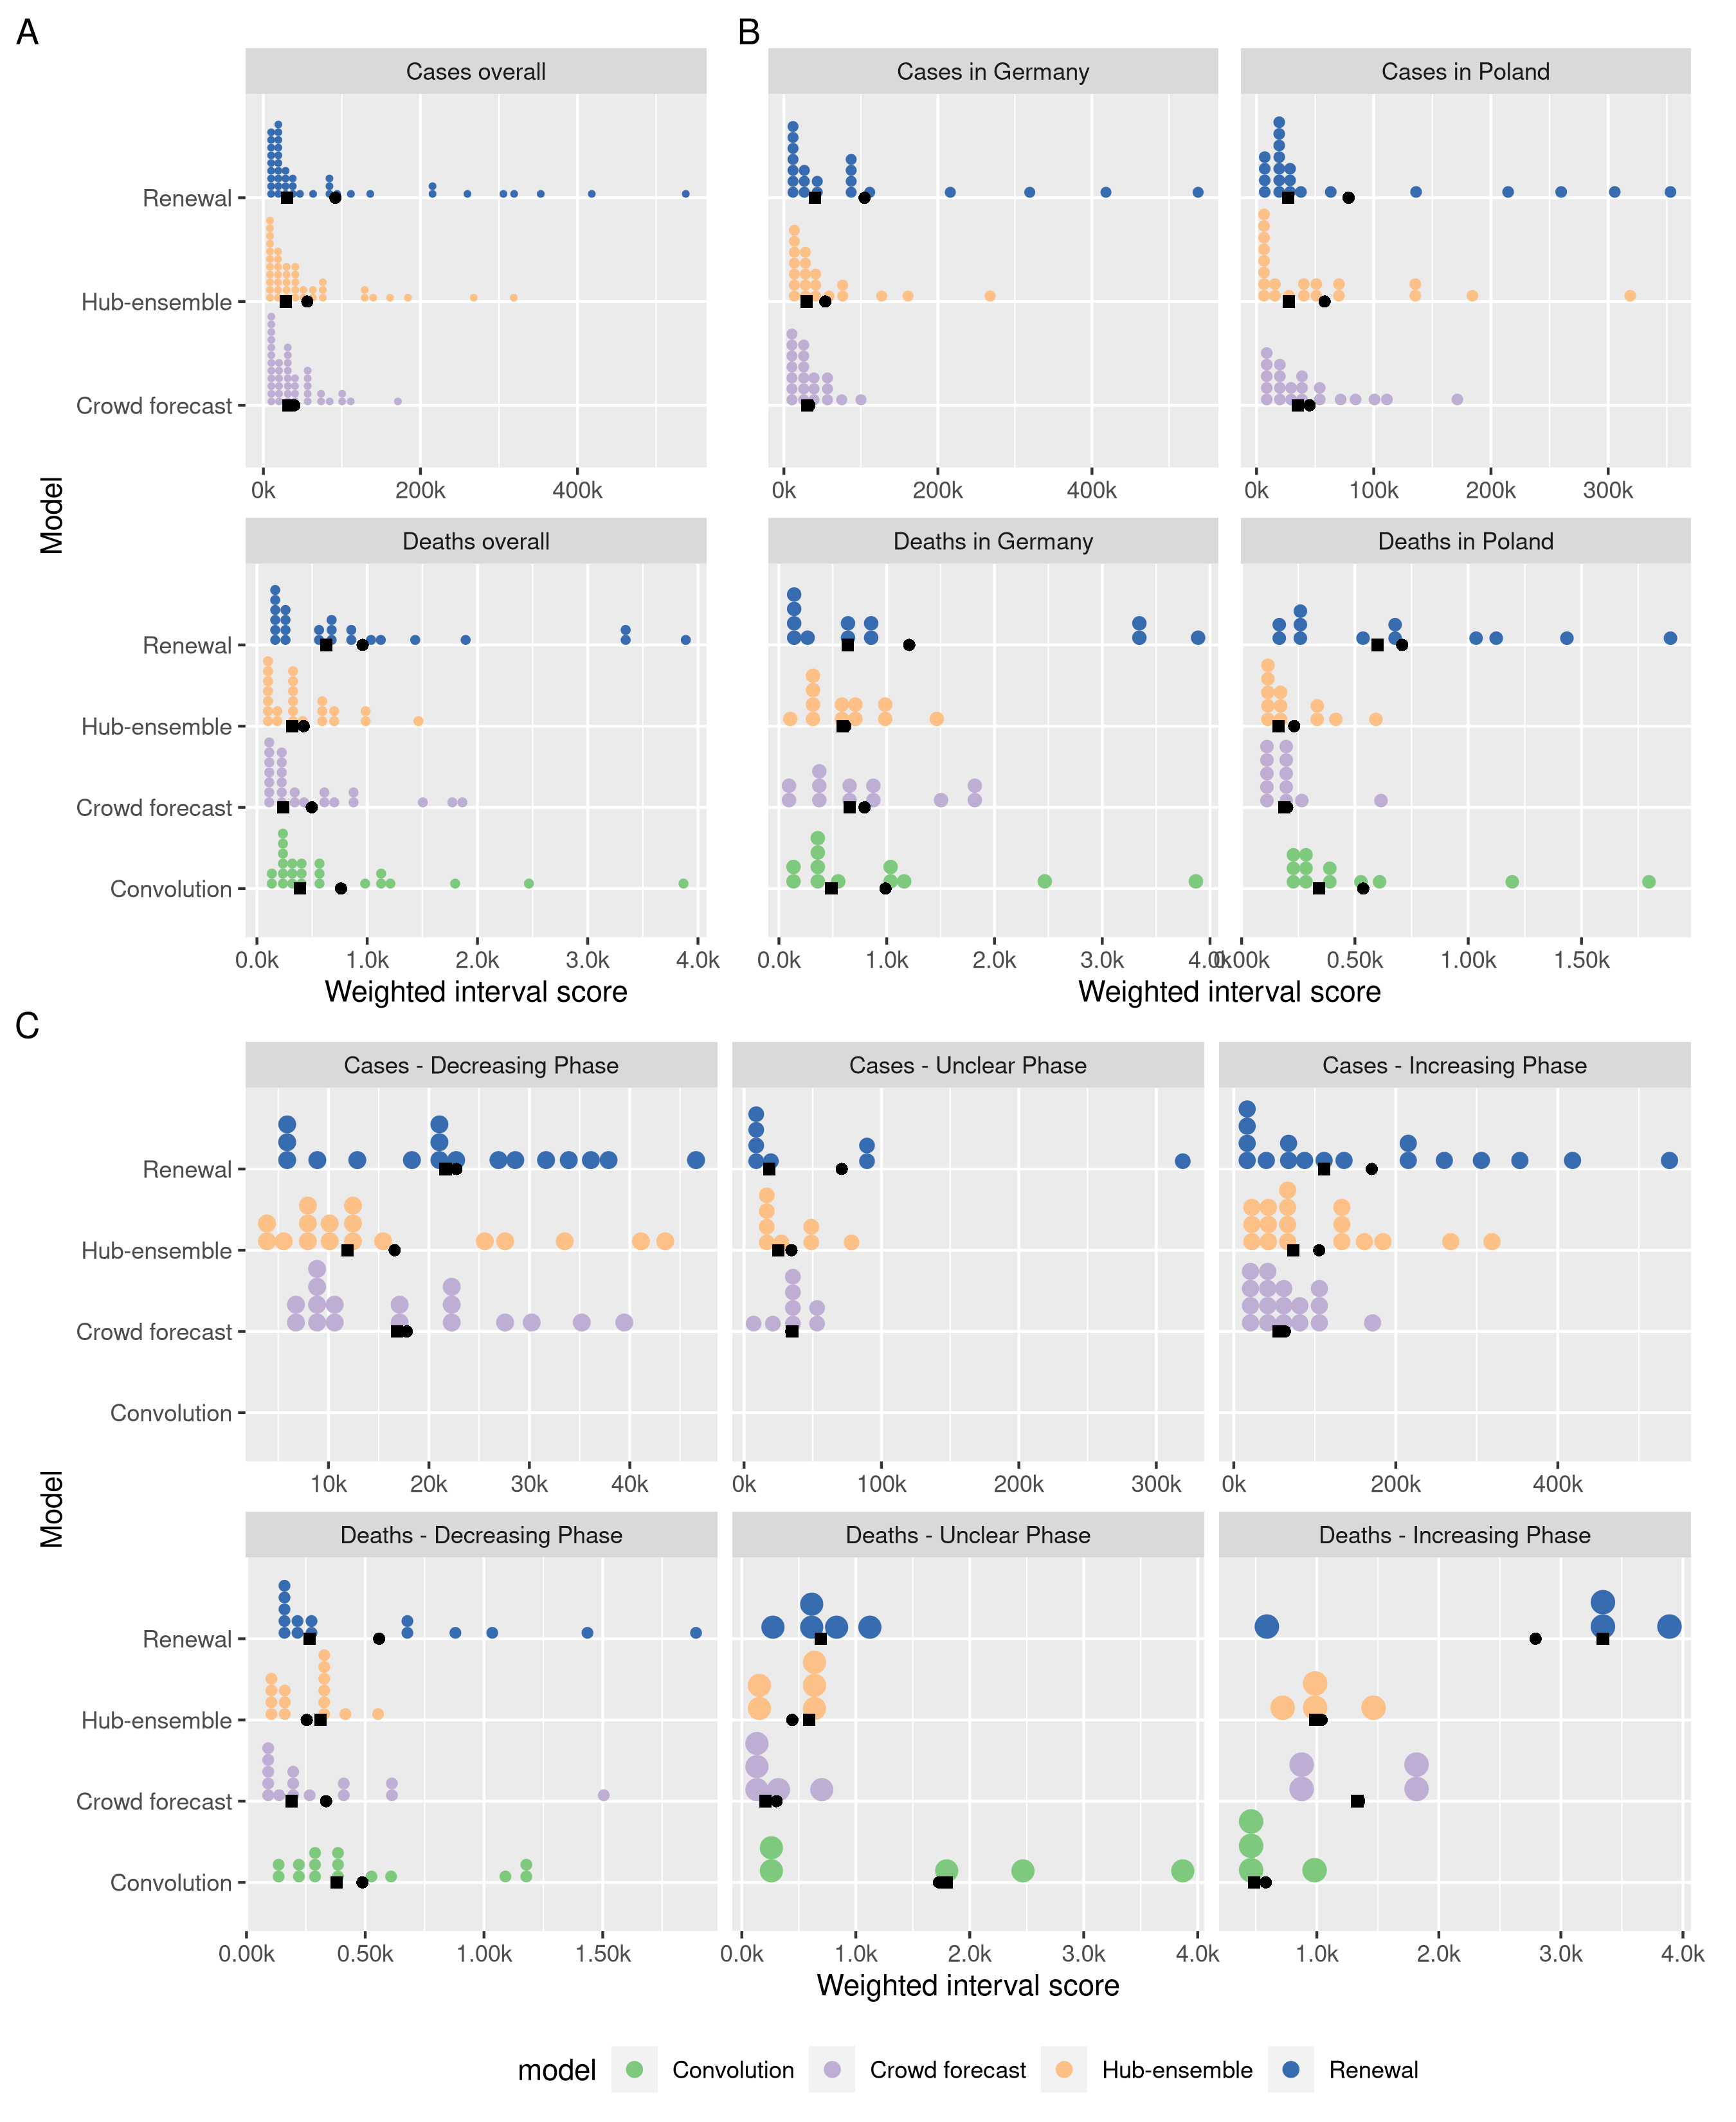
\includegraphics[width=1\linewidth,]{../analysis/plots/distribution_scores_wis-4} \caption{A: Distribution of weighted interval scores for four week ahead forecasts of the different models and forecast targets. B: Distribution of WIS separate by country.}\label{fig:distribution-scores-4}
\end{figure}

\hypertarget{ranks-achieved-by-forecasts}{%
\subsubsection{Ranks achieved by forecasts}\label{ranks-achieved-by-forecasts}}

\begin{figure}[H]
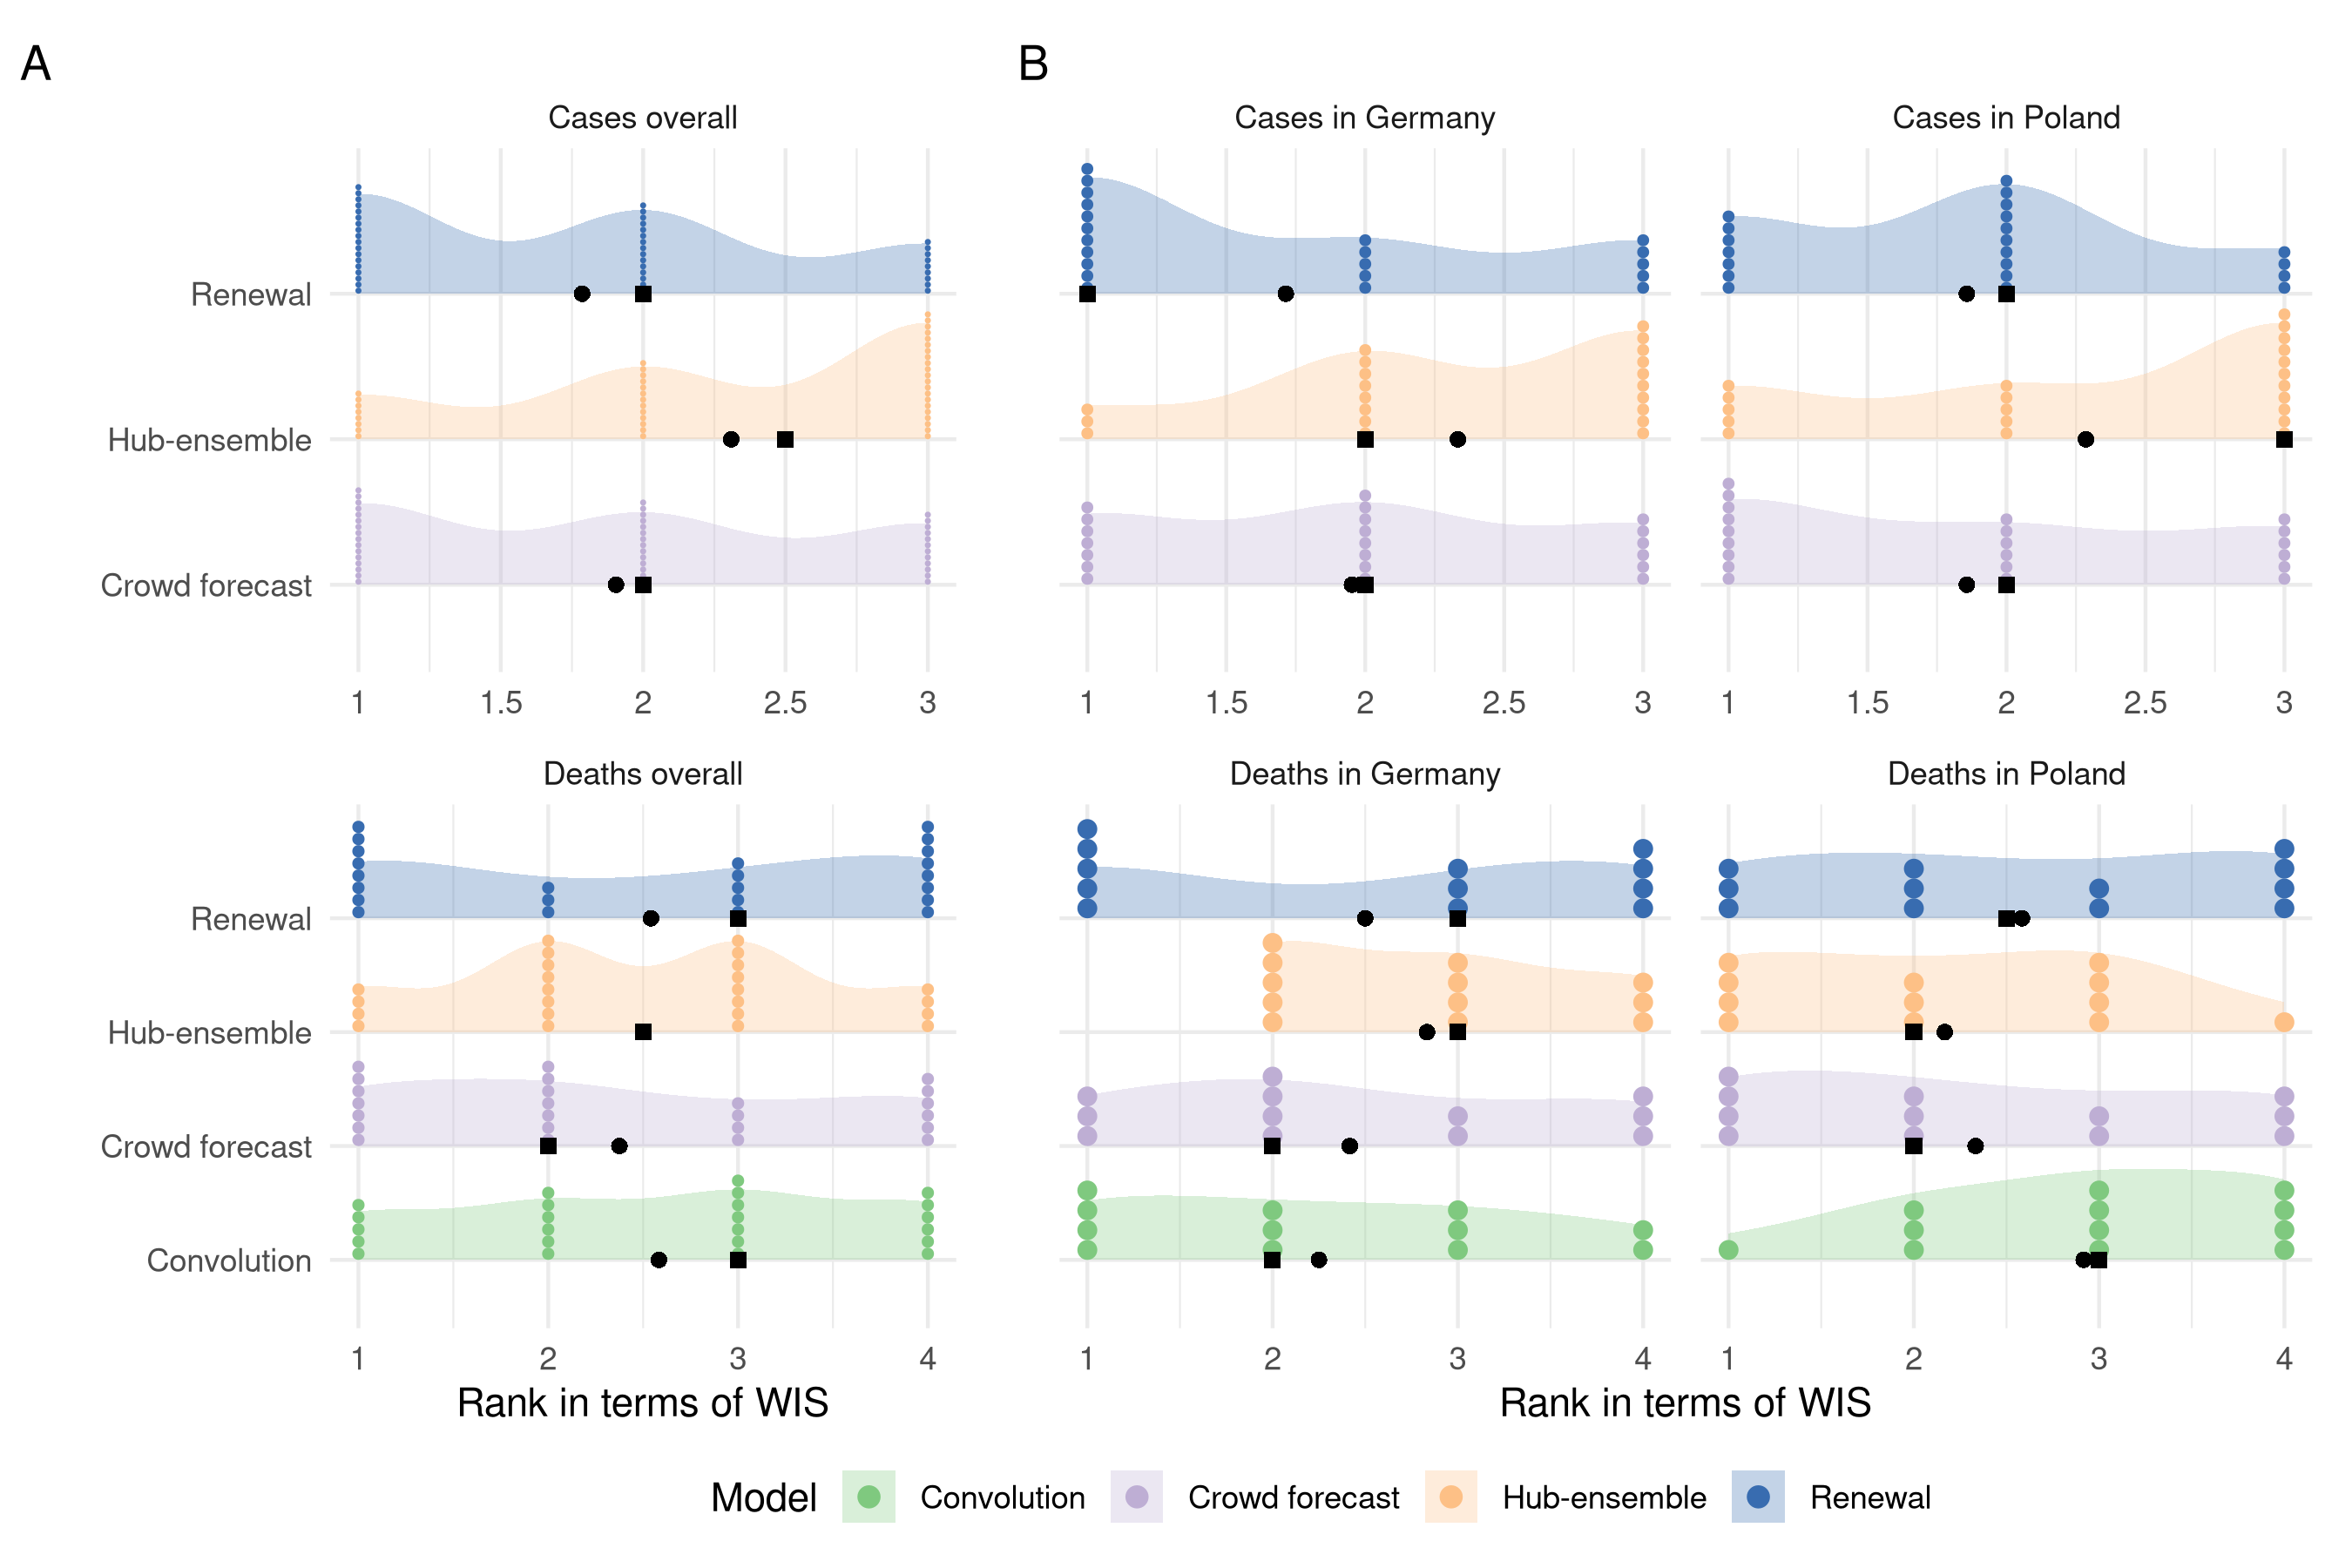
\includegraphics[width=1\linewidth,]{../analysis/plots/distribution_scores_wis-1-ranks} \caption{A: Distribution of the ranks (determined by the weighted interval score) for one week ahead forecasts of the different models and forecast targets. B: Distribution of ranks separate by country.}\label{fig:distribution-scores-ranks-1}
\end{figure}

\begin{figure}[H]
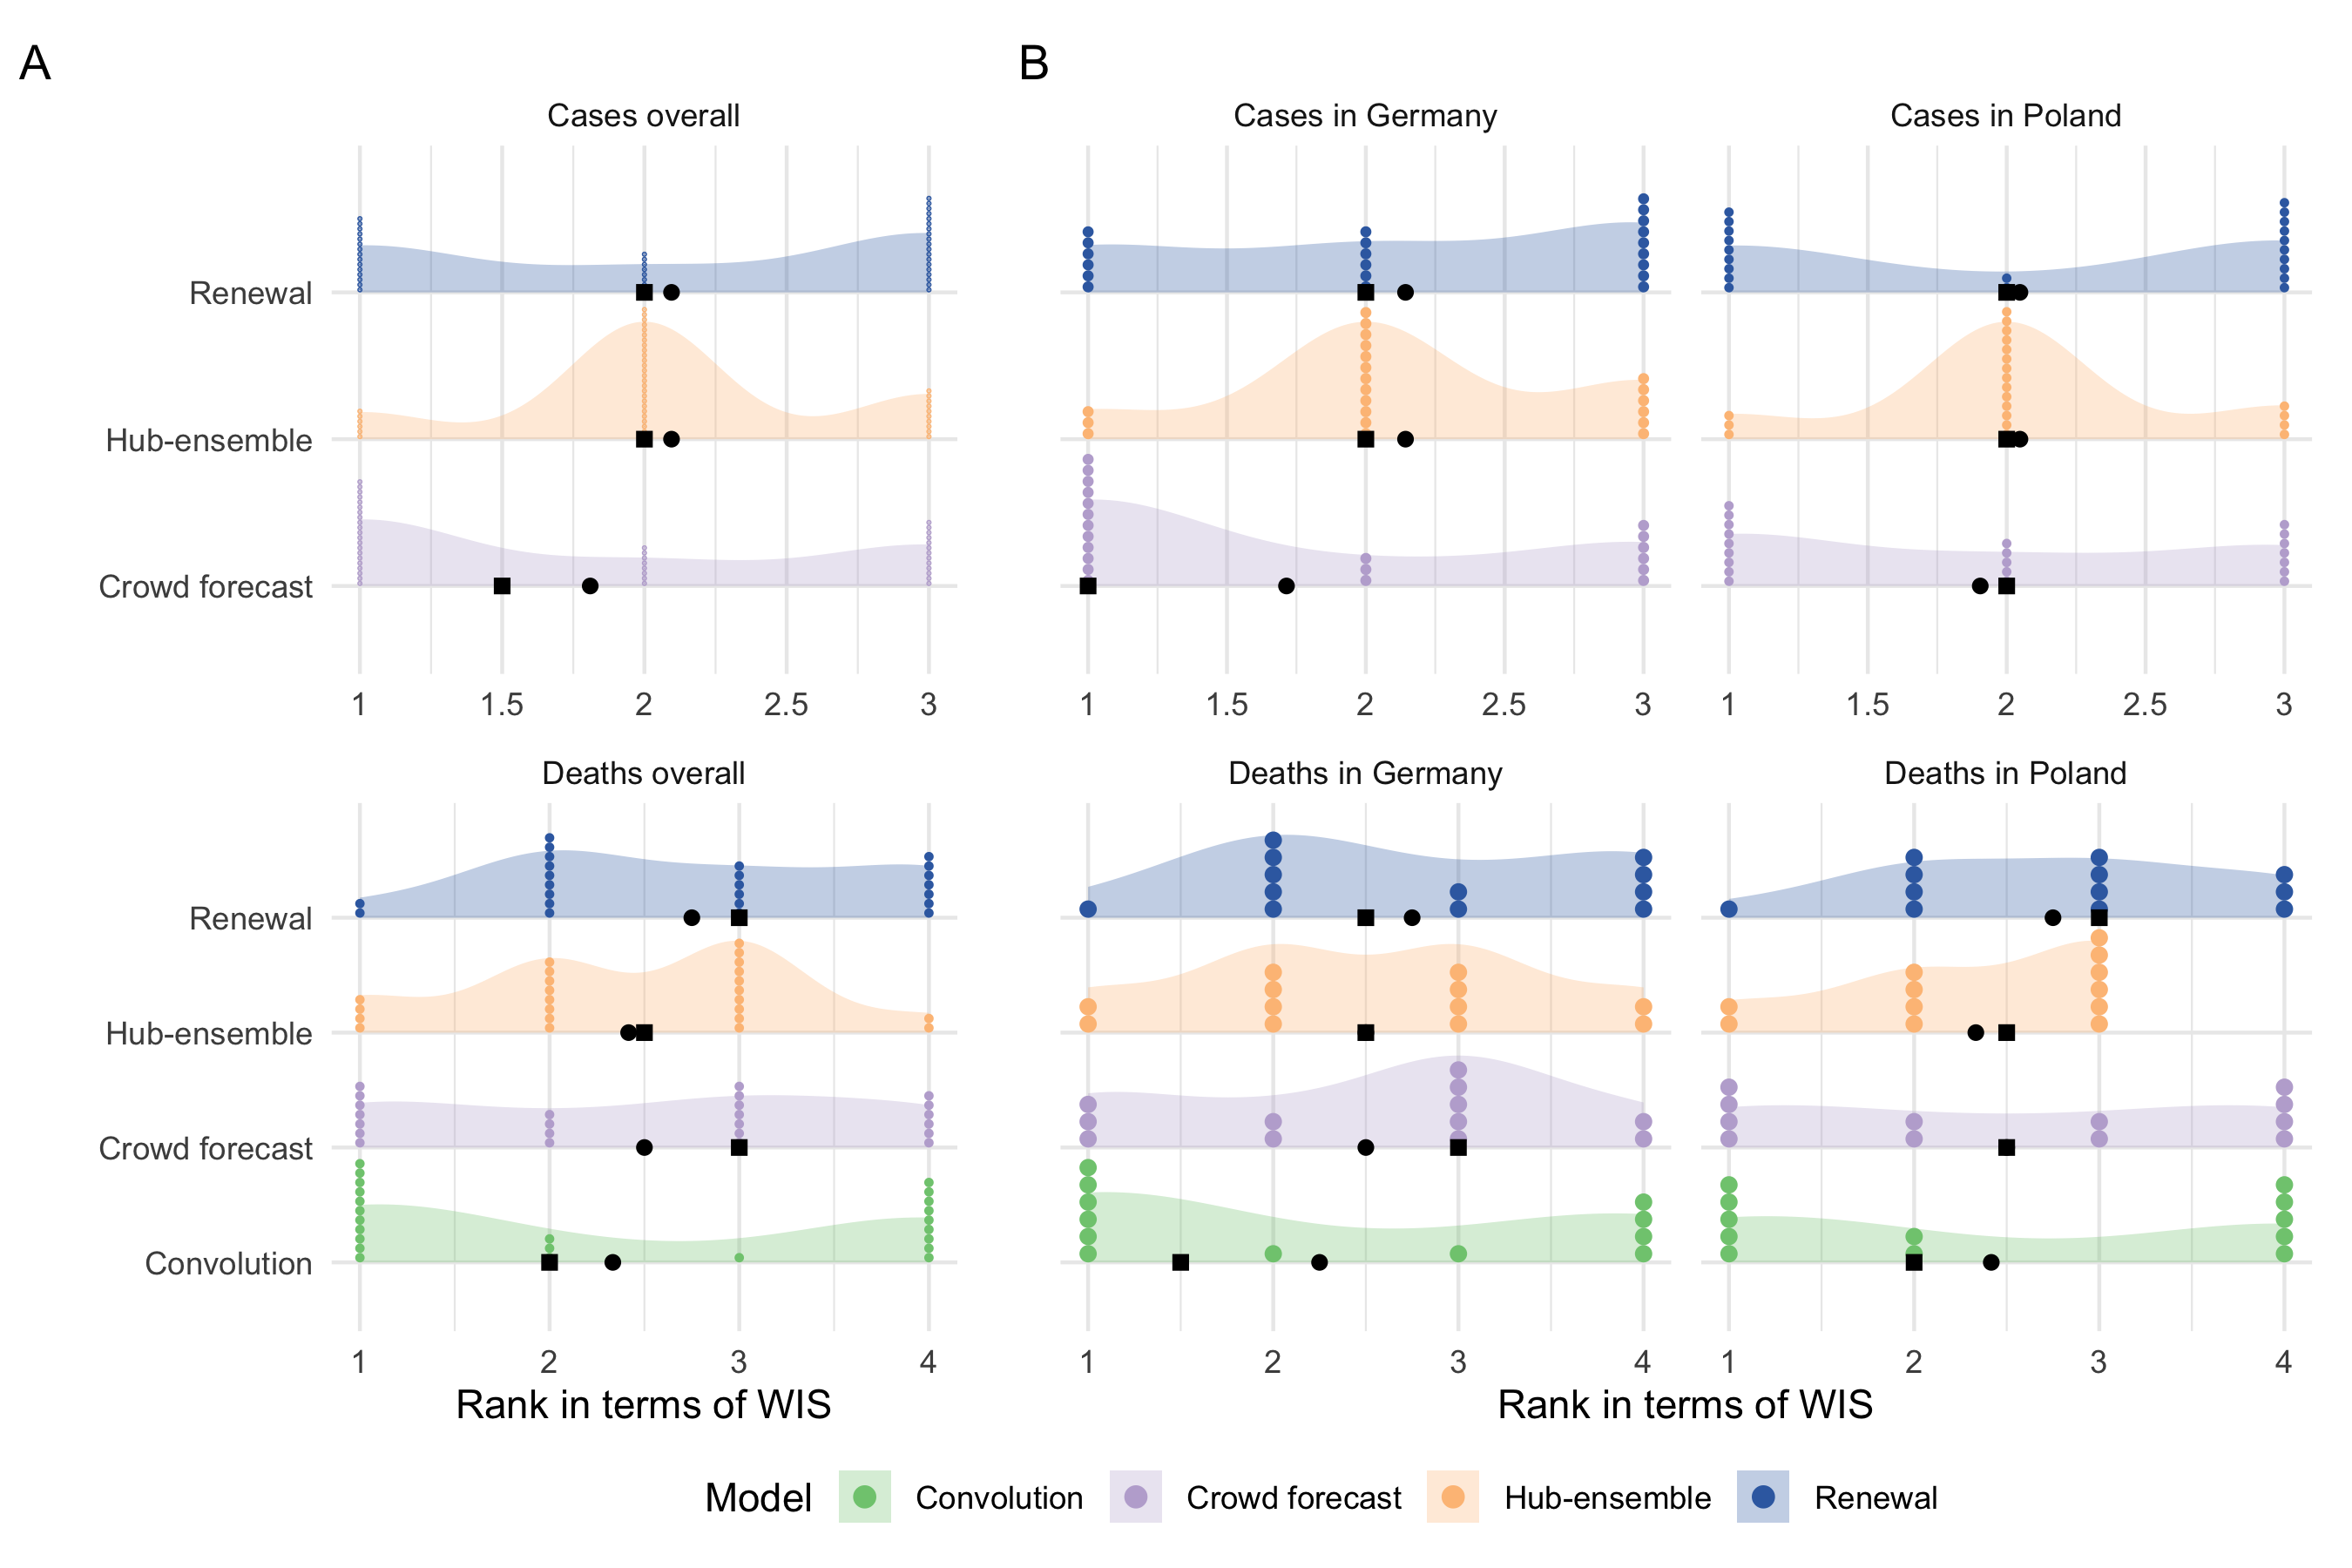
\includegraphics[width=1\linewidth,]{../analysis/plots/distribution_scores_wis-2-ranks} \caption{A: Distribution of the ranks (determined by the weighted interval score) for two week ahead forecasts of the different models and forecast targets. B: Distribution of ranks separate by country.}\label{fig:distribution-scores-ranks-2}
\end{figure}

\begin{figure}[H]
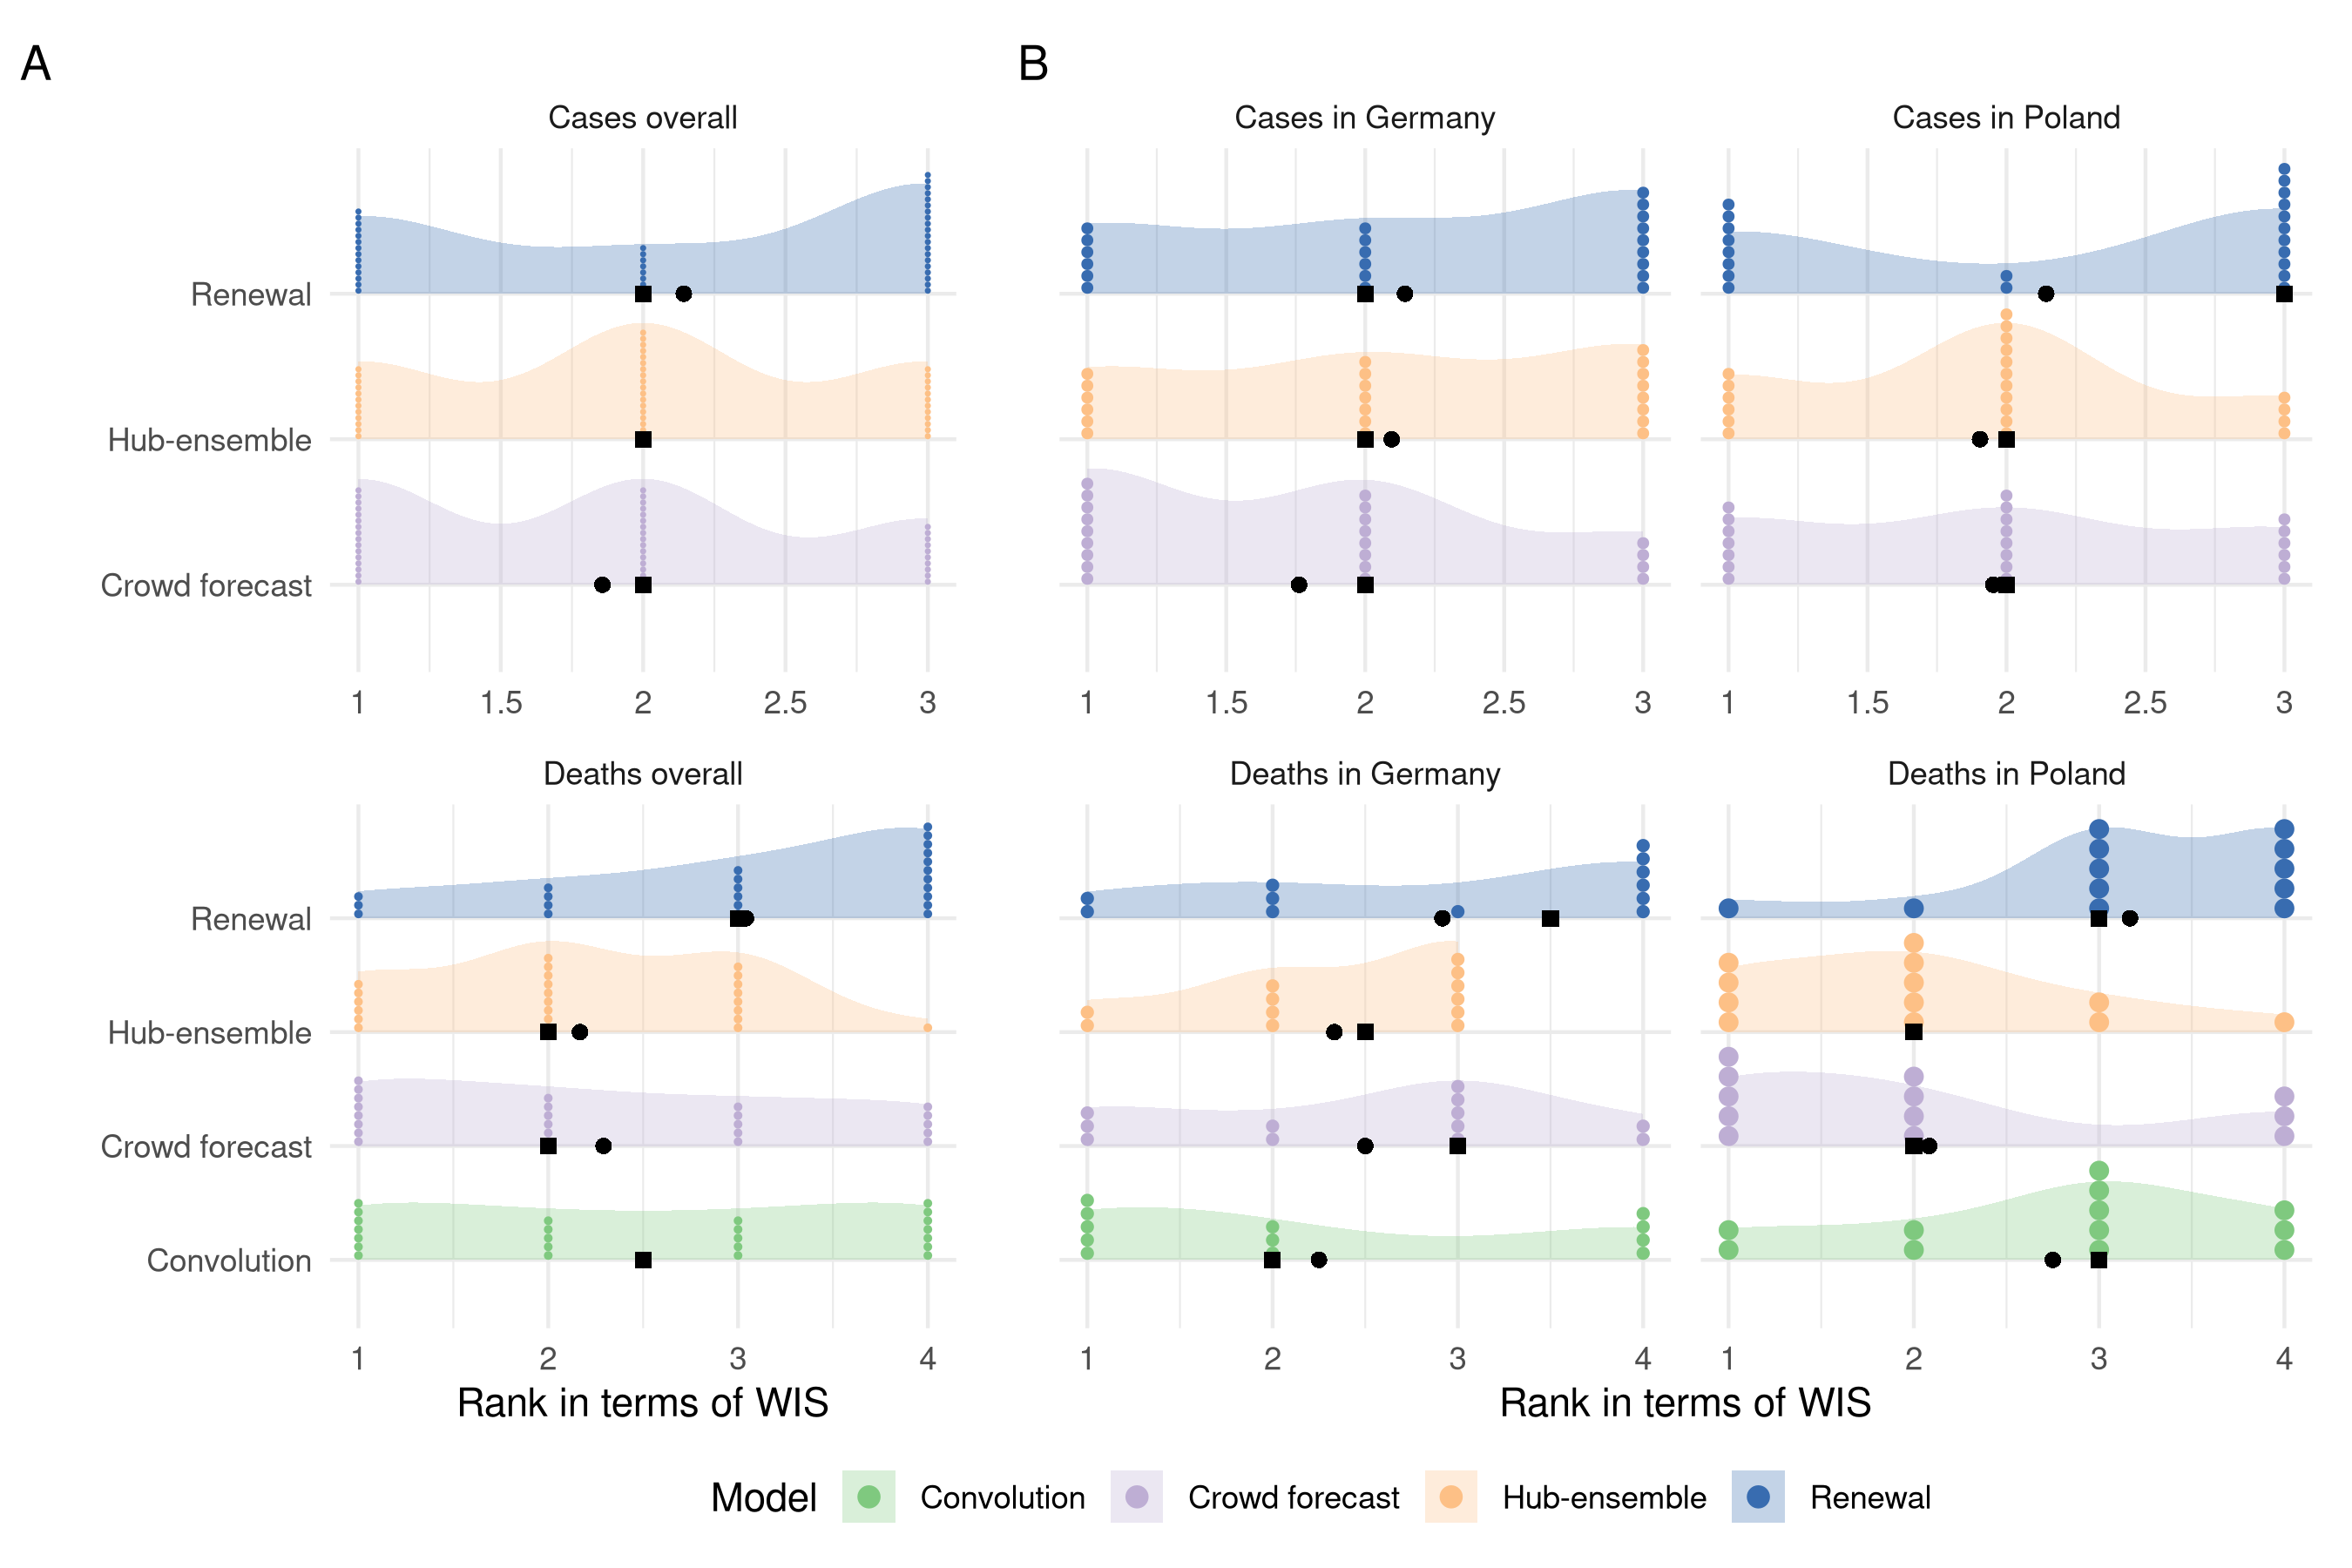
\includegraphics[width=1\linewidth,]{../analysis/plots/distribution_scores_wis-3-ranks} \caption{A: Distribution of the ranks (determined by the weighted interval score) for three week ahead forecasts of the different models and forecast targets. B: Distribution of ranks separate by country.}\label{fig:distribution-scores-ranks-3}
\end{figure}

\begin{figure}[H]
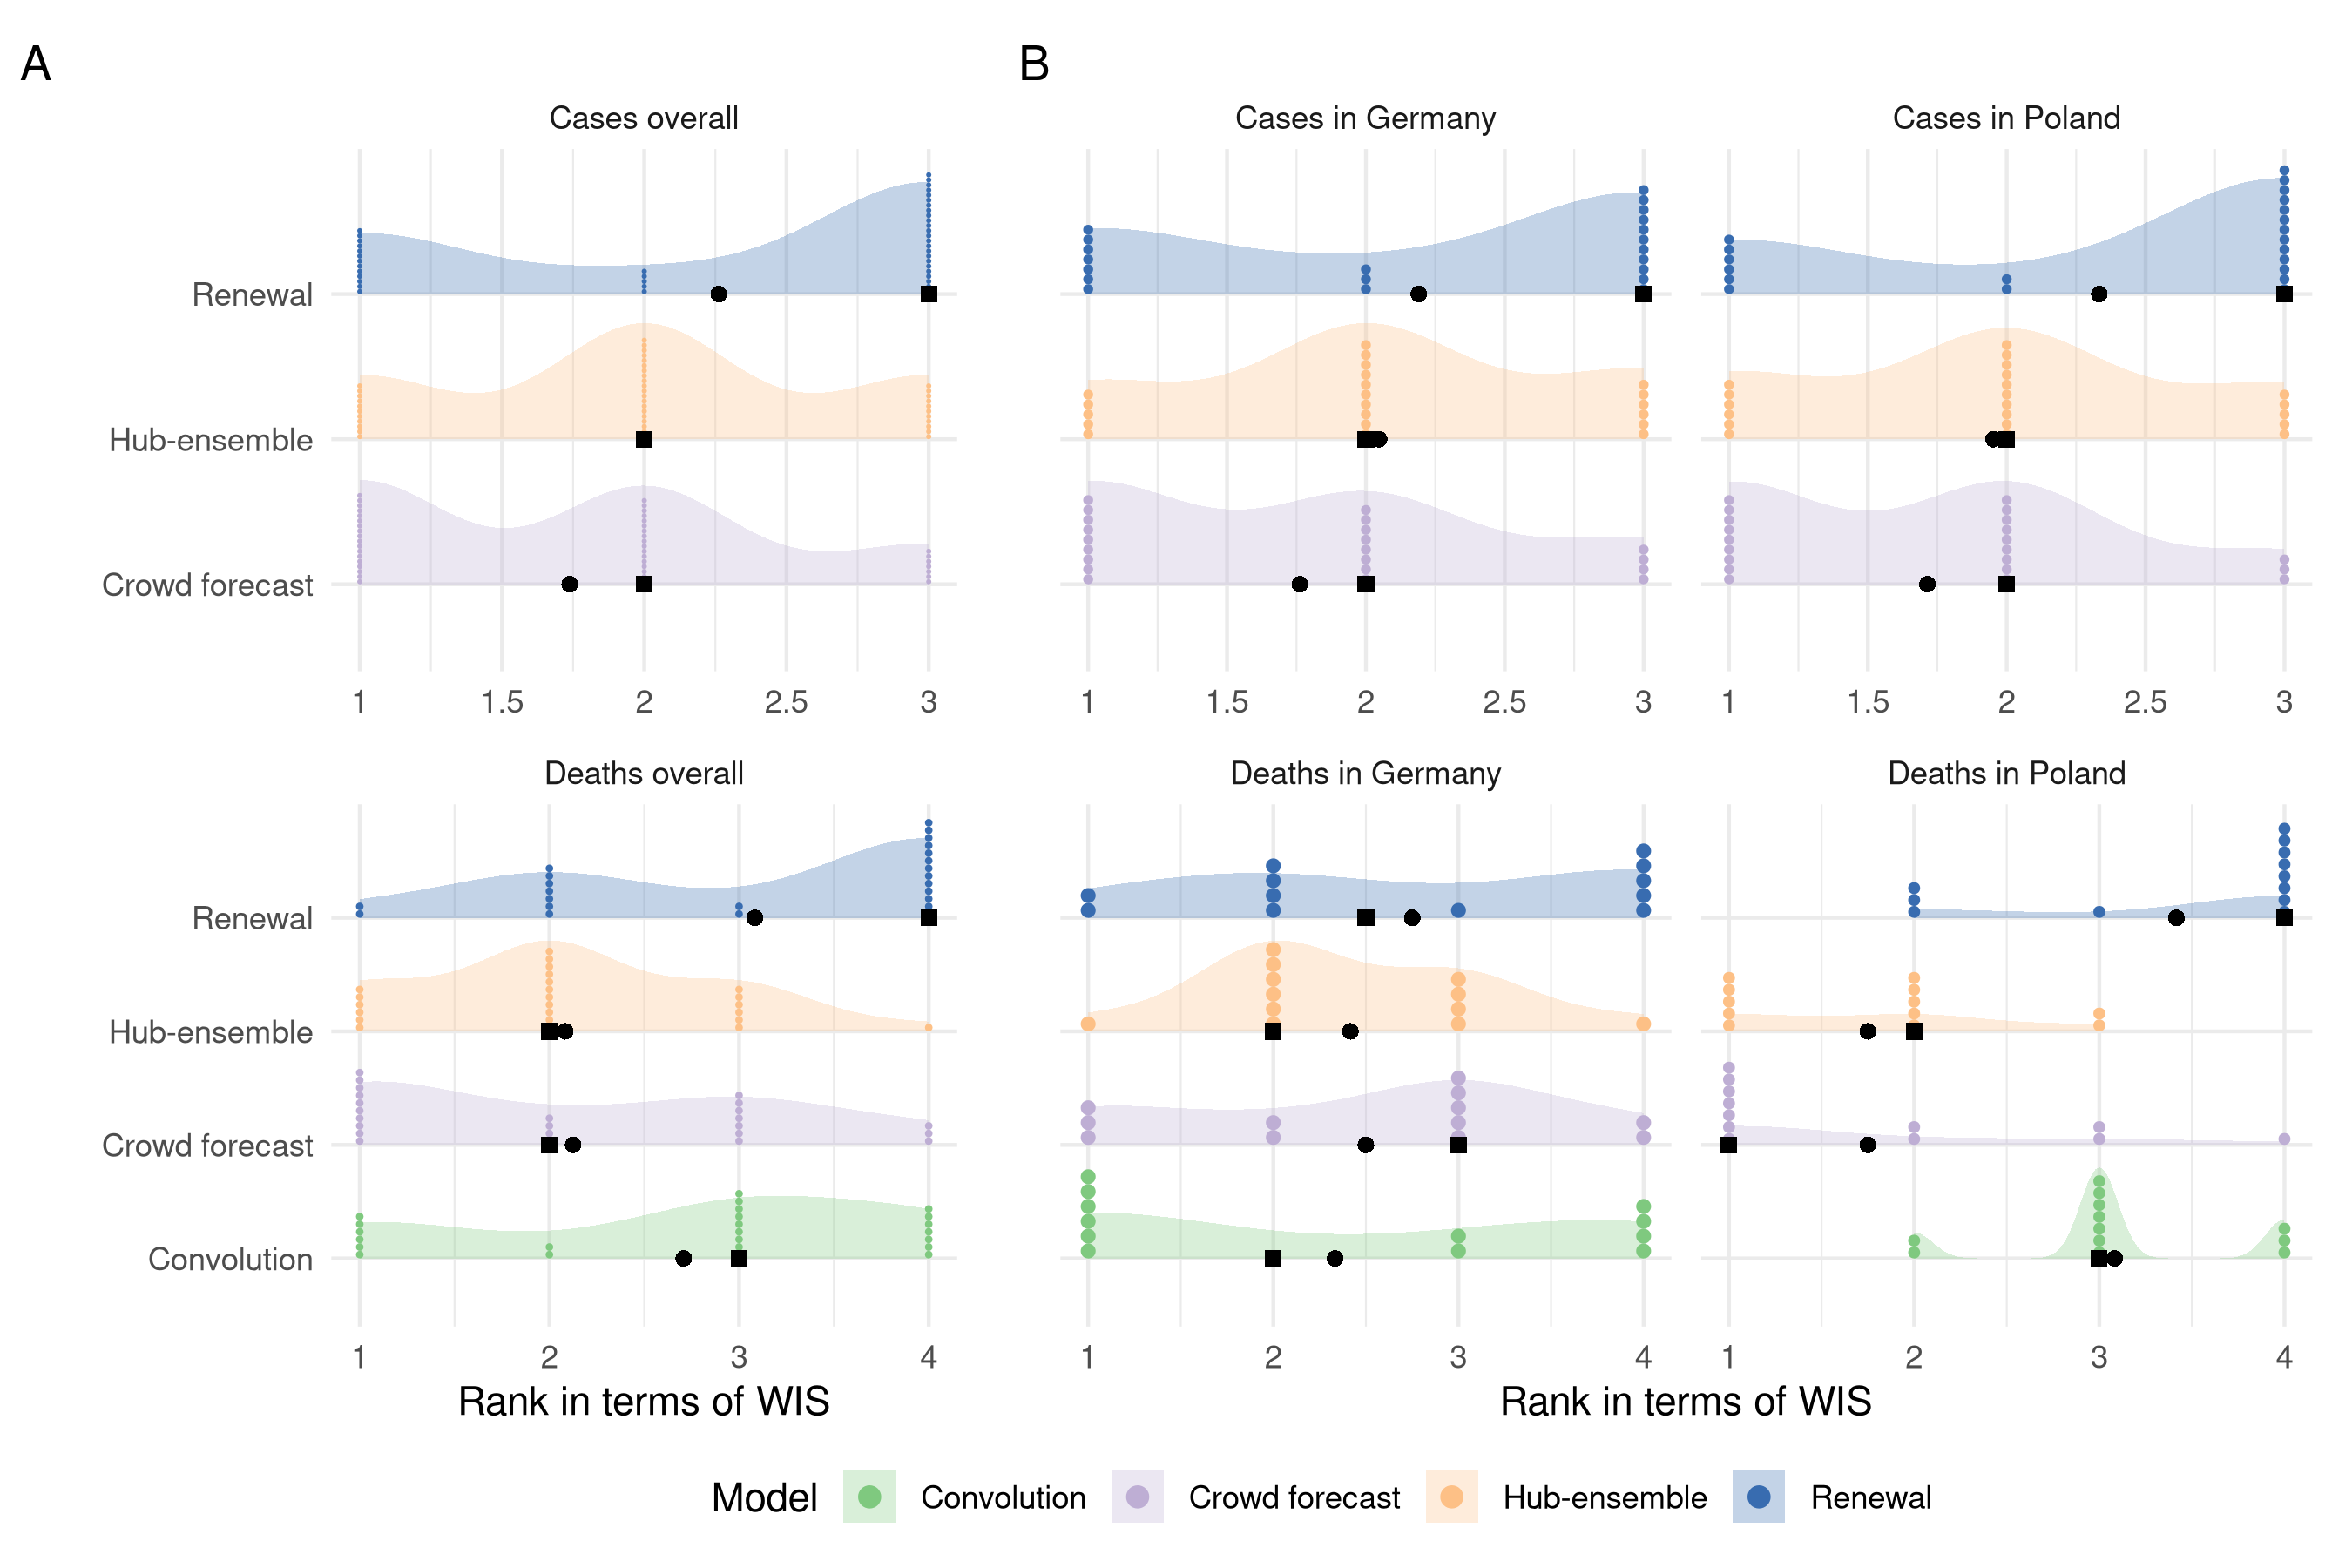
\includegraphics[width=1\linewidth,]{../analysis/plots/distribution_scores_wis-4-ranks} \caption{A: Distribution of the ranks (determined by the weighted interval score) for four week ahead forecasts of the different models and forecast targets. B: Distribution of ranks separate by country.}\label{fig:distribution-scores-ranks-4}
\end{figure}

\clearpage

\hypertarget{comparison-of-ensembles}{%
\subsection{Comparison of ensembles}\label{comparison-of-ensembles}}

\hypertarget{performance-visualisation-mean-ensemble}{%
\subsubsection{Performance visualisation mean ensemble}\label{performance-visualisation-mean-ensemble}}

\begin{figure}[H]
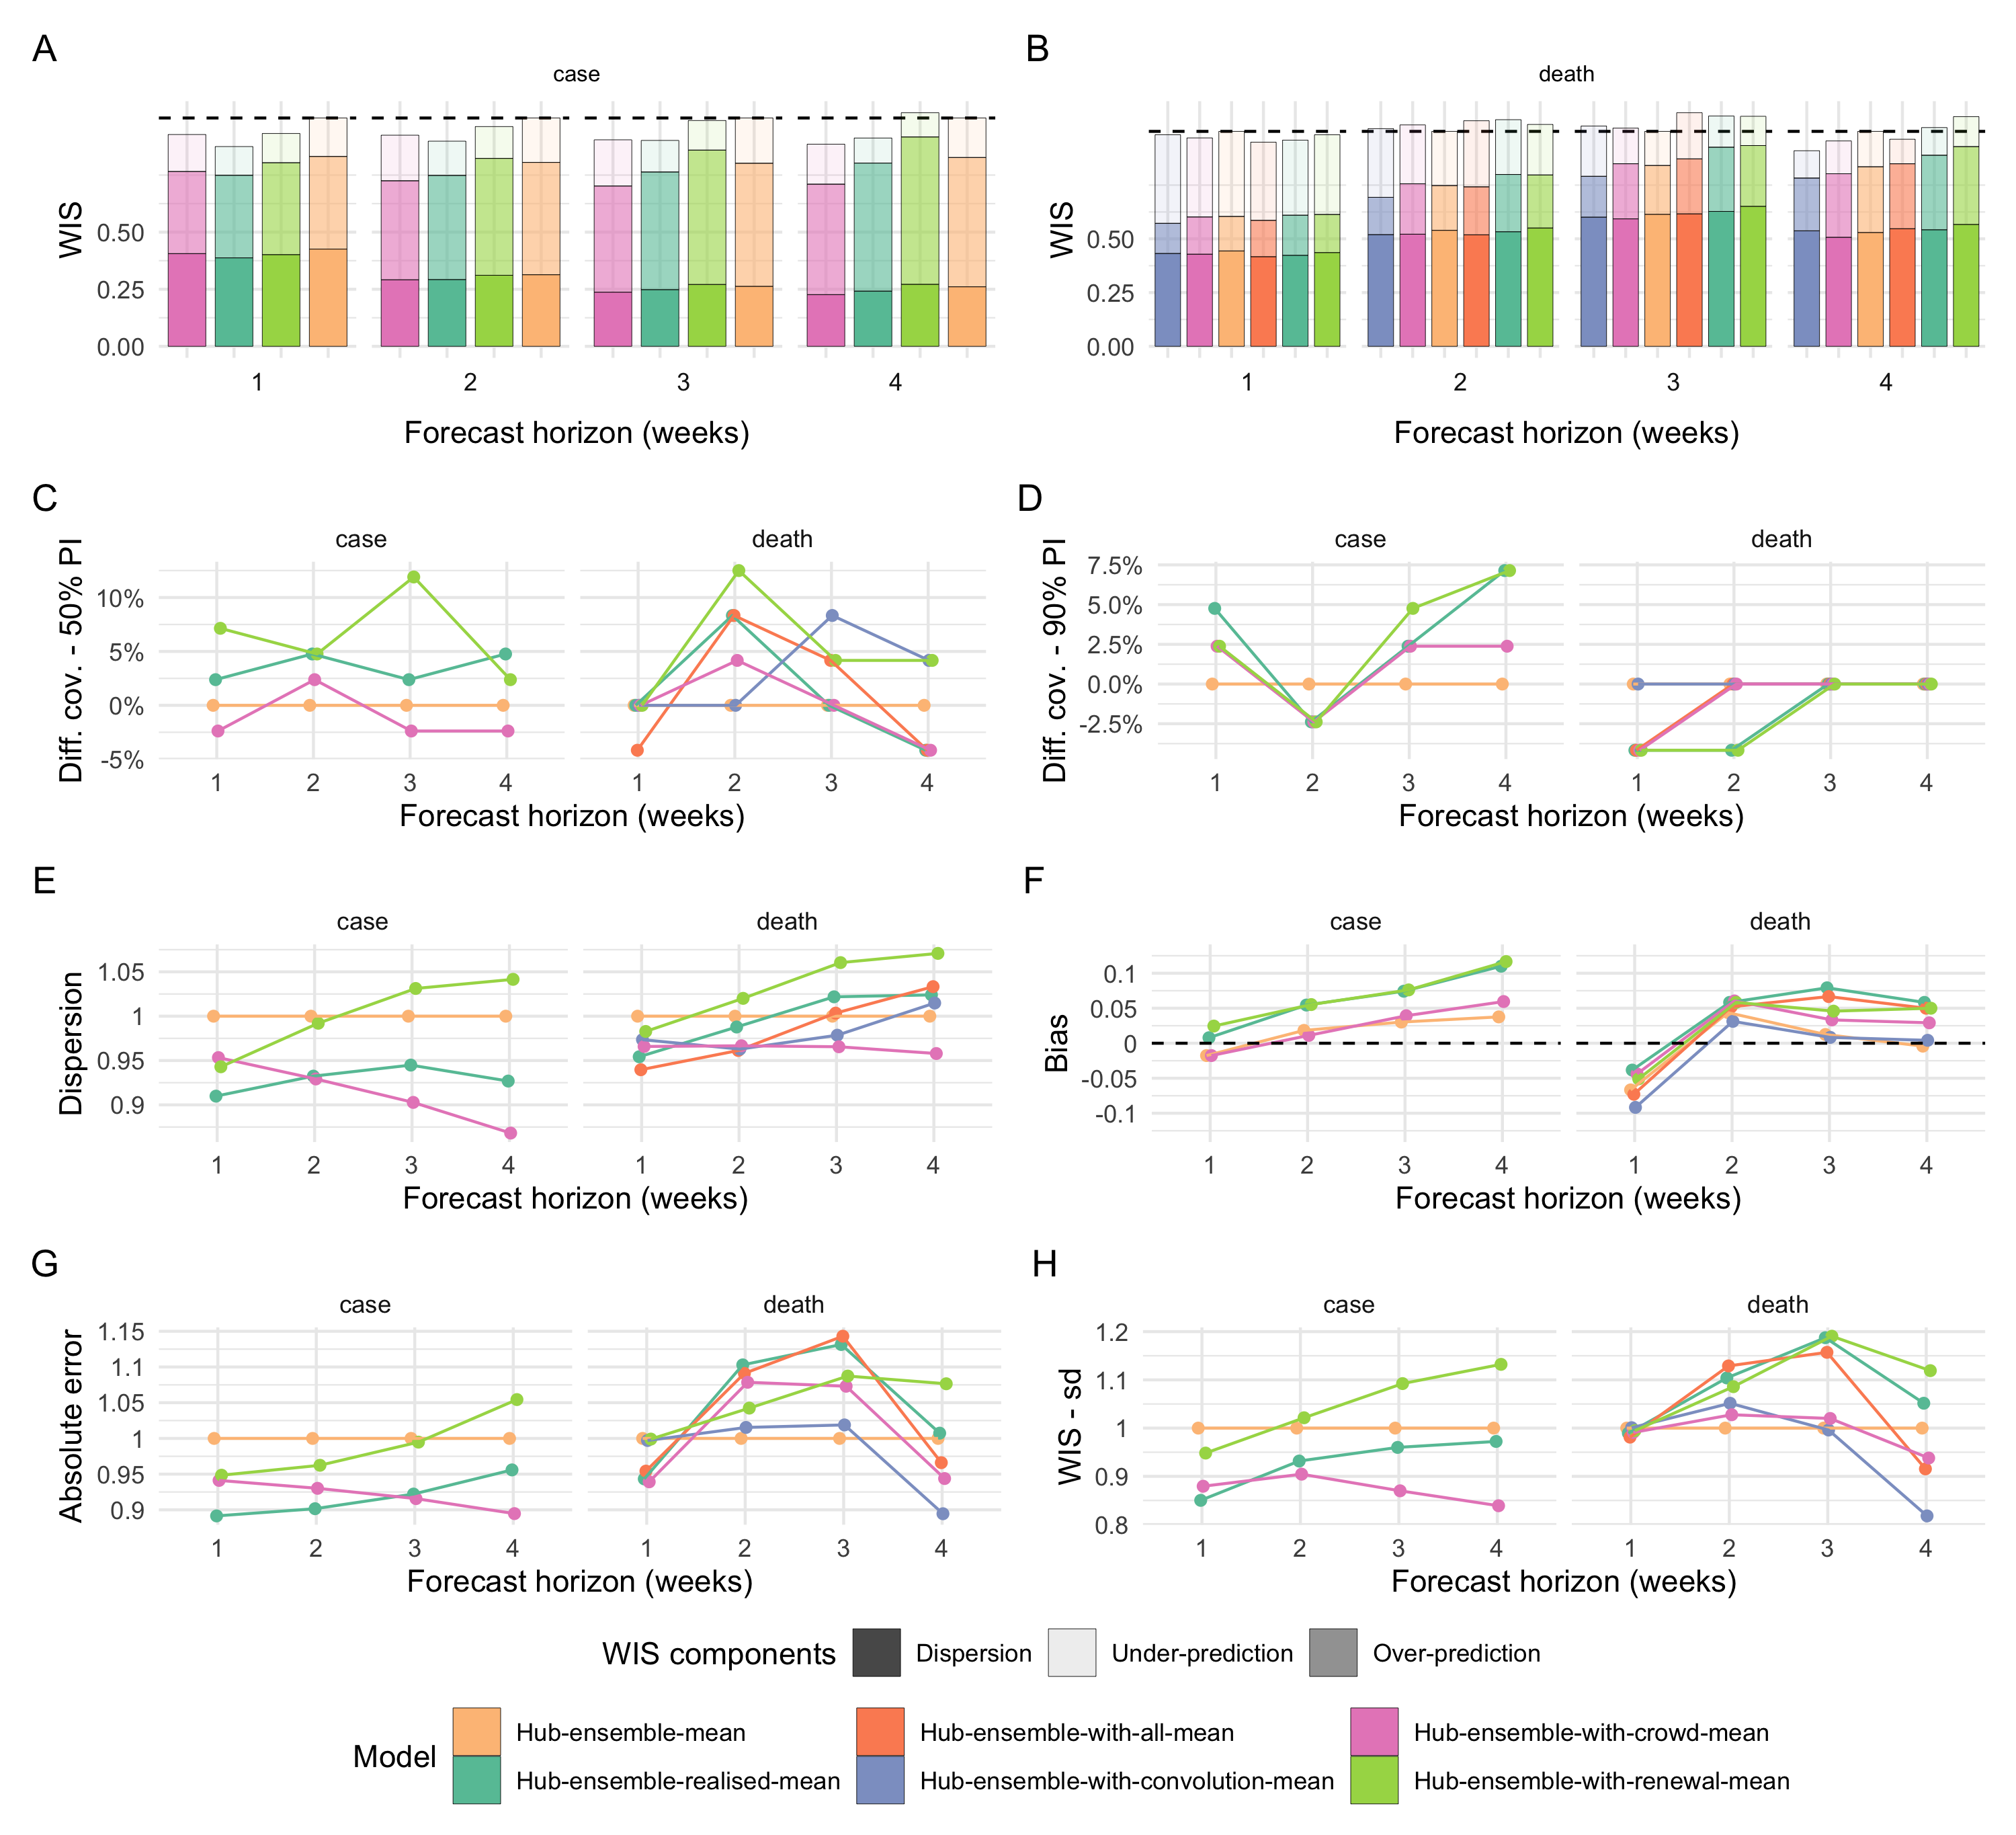
\includegraphics[width=1\linewidth,]{../analysis/plots/aggregate-performance-rel-ensemble-mean-v4} \caption{Visualisation of aggregate performance metrics across forecast horizons for the different versions of the Hub mean ensemble. “Hub-ensemble” excludes all our models, Hub-ensemble-all includes all of our models, “Hub-ensemble-real” is the real hub-ensemble with the renewal model and the crowd forecasts included. Values (except for Bias) are computed as differences to the Hub ensemble excluding our contributions. For Coverage, this is an absolute difference, for other metrics this is a percentage difference. A: mean weighted interval score (WIS) across horizons. B: median WIS. C: Absolute error of the median forecast. D: Standard deviation of the WIS. E: Dispersion (higher values mean greater spread of the forecast). F: Bias, i.e. general tendency to over- or underpredict. Values are between -1 (complete under-prediction) and 1 (complete over-prediction) and 0 ideally. G: Empirical coverage of the 50\% prediction intervals. F: Empirical coverage of the 90\% prediction intervals}\label{fig:agg-performance-ensemble-mean}
\end{figure}

\hypertarget{tables-median-ensemble}{%
\subsubsection{Tables median ensemble}\label{tables-median-ensemble}}

\begin{table}[!h]
\caption{\label{tab:score-table-ensemble-2}Scores for one and two week ahead forecasts (cut to three significant digits and rounded) for the different versions of the median ensemble. Note that scores for cases (which include the whole period from October 12th 2020 until March 1st 2021) and deaths (which include only forecasts from the 21st of December 2020 on) are computed on different subsets. Numbers in brackets show the metrics relative to the Hub ensemble (i.e. the median ensemble of all other models submitted to the German and Polish Forecast Hub, excluding our contributions). WIS is the mean weighted interval score (lower values are better), WIS - sd is the standard deviation of all scores achieved by a model. Dispersion, over-prediction and under-prediction together sum up to the weighted interval score. Bias (between -1 and 1, 0 is ideal) represents the general average tendency of a model to over- or underpredict. 50\% and 90\%-coverage are the percentage of observed values that fell within the 50\% and 90\% prediction intervals of a model.\\\hspace{\textwidth}}

\centering
\resizebox{\linewidth}{!}{
\begin{tabular}{>{}llccccccccc}
\toprule
  & Model & WIS & WIS - sd & dispersion & Underpred. & Overpred. & Bias & Abs. error & 50\%-Cov. & 90\%-Cov.\\
\midrule
\addlinespace[0.3em]
\multicolumn{11}{l}{\textbf{Cases}}\\
\hline
\cellcolor{white}{} & Hub-ensemble & 8770 (1) & 11700 (1) & 3670 (1) & 1230 (1) & 3870 (1) & -0.04 & 12700 (1) & 0.57 & 0.81\\
\cmidrule{2-11}
\cellcolor{white}{} & Hub-ensemble-realised & 6970 (0.79) & 8260 (0.71) & 3060 (0.83) & 943 (0.77) & 2970 (0.77) & 0.04 & 10800 (0.85) & 0.55 & 0.83\\
\cmidrule{2-11}
\cellcolor{white}{} & Hub-ensemble-with-crowd & 7820 (0.89) & 9630 (0.82) & 3270 (0.89) & 1210 (0.98) & 3330 (0.86) & -0.02 & 12000 (0.94) & 0.48 & 0.81\\
\cmidrule{2-11}
\cellcolor{white}{\multirow{-4}{*}{\raggedright\arraybackslash 1 wk ahead}} & Hub-ensemble-with-renewal & 7960 (0.91) & 10300 (0.88) & 3190 (0.87) & 1020 (0.83) & 3760 (0.97) & 0.04 & 12100 (0.95) & 0.57 & 0.83\\
\cmidrule{1-11}
\cellcolor{white}{} & Hub-ensemble & 18300 (1) & 21900 (1) & 6140 (1) & 3800 (1) & 8410 (1) & -0.03 & 26800 (1) & 0.43 & 0.64\\
\cmidrule{2-11}
\cellcolor{white}{} & Hub-ensemble-realised & 16400 (0.9) & 19600 (0.89) & 5350 (0.87) & 3290 (0.87) & 7730 (0.92) & 0.02 & 24200 (0.9) & 0.43 & 0.69\\
\cmidrule{2-11}
\cellcolor{white}{} & Hub-ensemble-with-crowd & 16900 (0.92) & 19600 (0.89) & 5230 (0.85) & 4310 (1.13) & 7370 (0.88) & 0.00 & 24600 (0.92) & 0.38 & 0.64\\
\cmidrule{2-11}
\cellcolor{white}{\multirow{-4}{*}{\raggedright\arraybackslash 2 wk ahead}} & Hub-ensemble-with-renewal & 17500 (0.96) & 21400 (0.98) & 5830 (0.95) & 2880 (0.76) & 8770 (1.04) & 0.00 & 25500 (0.95) & 0.45 & 0.71\\
\cmidrule{1-11}
\addlinespace[0.3em]
\multicolumn{11}{l}{\textbf{Deaths}}\\
\hline
\cellcolor{white}{} & Hub-ensemble & 248 (1) & 338 (1) & 92.2 (1) & 115 (1) & 41.6 (1) & -0.04 & 334 (1) & 0.62 & 0.92\\
\cmidrule{2-11}
\cellcolor{white}{} & Hub-ensemble-realised & 235 (0.95) & 332 (0.98) & 88.6 (0.96) & 90.4 (0.79) & 55.5 (1.33) & -0.01 & 323 (0.97) & 0.62 & 0.88\\
\cmidrule{2-11}
\cellcolor{white}{} & Hub-ensemble-with-all & 234 (0.94) & 331 (0.98) & 85.2 (0.92) & 98.1 (0.85) & 50.2 (1.21) & -0.05 & 329 (0.99) & 0.62 & 0.92\\
\cmidrule{2-11}
\cellcolor{white}{} & Hub-ensemble-with-convolution & 234 (0.94) & 329 (0.97) & 90.7 (0.98) & 118 (1.03) & 25.3 (0.61) & -0.08 & 333 (1) & 0.62 & 0.92\\
\cmidrule{2-11}
\cellcolor{white}{} & Hub-ensemble-with-crowd & 239 (0.96) & 337 (1) & 85.2 (0.92) & 99.6 (0.87) & 54.2 (1.3) & -0.03 & 322 (0.96) & 0.62 & 0.92\\
\cmidrule{2-11}
\cellcolor{white}{\multirow{-6}{*}{\raggedright\arraybackslash 1 wk ahead}} & Hub-ensemble-with-renewal & 246 (0.99) & 342 (1.01) & 91.5 (0.99) & 106 (0.92) & 48.6 (1.17) & -0.06 & 342 (1.02) & 0.67 & 0.92\\
\cmidrule{1-11}
\cellcolor{white}{} & Hub-ensemble & 292 (1) & 385 (1) & 132 (1) & 108 (1) & 51.9 (1) & 0.01 & 429 (1) & 0.62 & 0.96\\
\cmidrule{2-11}
\cellcolor{white}{} & Hub-ensemble-realised & 296 (1.01) & 398 (1.03) & 125 (0.95) & 91 (0.84) & 80.2 (1.55) & 0.05 & 486 (1.13) & 0.58 & 0.92\\
\cmidrule{2-11}
\cellcolor{white}{} & Hub-ensemble-with-all & 303 (1.04) & 423 (1.1) & 115 (0.87) & 122 (1.13) & 66.1 (1.27) & 0.00 & 483 (1.13) & 0.62 & 0.88\\
\cmidrule{2-11}
\cellcolor{white}{} & Hub-ensemble-with-convolution & 270 (0.92) & 385 (1) & 121 (0.92) & 119 (1.1) & 29.9 (0.58) & -0.04 & 403 (0.94) & 0.58 & 0.96\\
\cmidrule{2-11}
\cellcolor{white}{} & Hub-ensemble-with-crowd & 303 (1.04) & 392 (1.02) & 122 (0.92) & 106 (0.98) & 74.6 (1.44) & 0.03 & 499 (1.16) & 0.58 & 0.92\\
\cmidrule{2-11}
\cellcolor{white}{\multirow{-6}{*}{\raggedright\arraybackslash 2 wk ahead}} & Hub-ensemble-with-renewal & 296 (1.01) & 397 (1.03) & 128 (0.97) & 97.1 (0.9) & 71.2 (1.37) & -0.01 & 462 (1.08) & 0.67 & 0.92\\
\bottomrule
\end{tabular}}
\end{table}

\begin{table}[!h]
\caption{\label{tab:score-table-ensemble-4}Scores for three and four week ahead forecasts (cut to three significant digits and rounded) for the different versions of the median ensemble. Note that scores for cases (which include the whole period from October 12th 2020 until March 1st 2021) and deaths (which include only forecasts from the 21st of December 2020 on) are computed on different subsets. Numbers in brackets show the metrics relative to the Hub ensemble (i.e. the median ensemble of all other models submitted to the German and Polish Forecast Hub, excluding our contributions). WIS is the mean weighted interval score (lower values are better), WIS - sd is the standard deviation of all scores achieved by a model. Dispersion, over-prediction and under-prediction together sum up to the weighted interval score. Bias (between -1 and 1, 0 is ideal) represents the general average tendency of a model to over- or underpredict. 50\% and 90\%-coverage are the percentage of observed values that fell within the 50\% and 90\% prediction intervals of a model.\\\hspace{\textwidth}}

\centering
\resizebox{\linewidth}{!}{
\begin{tabular}{>{}llccccccccc}
\toprule
  & Model & WIS & WIS - sd & dispersion & Underpred. & Overpred. & Bias & Abs. error & 50\%-Cov. & 90\%-Cov.\\
\midrule
\addlinespace[0.3em]
\multicolumn{11}{l}{\textbf{Cases}}\\
\hline
\cellcolor{white}{} & Hub-ensemble & 33400 (1) & 40700 (1) & 9130 (1) & 7690 (1) & 16600 (1) & -0.01 & 46900 (1) & 0.29 & 0.62\\
\cmidrule{2-11}
\cellcolor{white}{} & Hub-ensemble-realised & 30800 (0.92) & 38600 (0.95) & 7910 (0.87) & 6890 (0.9) & 16000 (0.96) & 0.03 & 44200 (0.94) & 0.29 & 0.62\\
\cmidrule{2-11}
\cellcolor{white}{} & Hub-ensemble-with-crowd & 30800 (0.92) & 34100 (0.84) & 7500 (0.82) & 8960 (1.17) & 14300 (0.86) & 0.02 & 44100 (0.94) & 0.24 & 0.55\\
\cmidrule{2-11}
\cellcolor{white}{\multirow{-4}{*}{\raggedright\arraybackslash 3 wk ahead}} & Hub-ensemble-with-renewal & 34000 (1.02) & 43100 (1.06) & 8860 (0.97) & 6300 (0.82) & 18900 (1.14) & 0.02 & 48100 (1.03) & 0.29 & 0.60\\
\cmidrule{1-11}
\cellcolor{white}{} & Hub-ensemble & 55900 (1) & 73700 (1) & 12200 (1) & 12400 (1) & 31300 (1) & 0.01 & 74400 (1) & 0.24 & 0.52\\
\cmidrule{2-11}
\cellcolor{white}{} & Hub-ensemble-realised & 51200 (0.92) & 69900 (0.95) & 10900 (0.89) & 11100 (0.9) & 29300 (0.94) & 0.04 & 69600 (0.94) & 0.19 & 0.57\\
\cmidrule{2-11}
\cellcolor{white}{} & Hub-ensemble-with-crowd & 48800 (0.87) & 58600 (0.8) & 9700 (0.8) & 13700 (1.1) & 25400 (0.81) & 0.00 & 65800 (0.88) & 0.19 & 0.48\\
\cmidrule{2-11}
\cellcolor{white}{\multirow{-4}{*}{\raggedright\arraybackslash 4 wk ahead}} & Hub-ensemble-with-renewal & 59100 (1.06) & 84100 (1.14) & 12600 (1.03) & 10100 (0.81) & 36400 (1.16) & 0.01 & 78900 (1.06) & 0.29 & 0.55\\
\cmidrule{1-11}
\addlinespace[0.3em]
\multicolumn{11}{l}{\textbf{Deaths}}\\
\hline
\cellcolor{white}{} & Hub-ensemble & 319 (1) & 328 (1) & 172 (1) & 92.7 (1) & 55.1 (1) & -0.03 & 488 (1) & 0.54 & 0.96\\
\cmidrule{2-11}
\cellcolor{white}{} & Hub-ensemble-realised & 332 (1.04) & 388 (1.18) & 158 (0.92) & 78.7 (0.85) & 95 (1.72) & -0.02 & 547 (1.12) & 0.46 & 1.00\\
\cmidrule{2-11}
\cellcolor{white}{} & Hub-ensemble-with-all & 321 (1.01) & 385 (1.17) & 153 (0.89) & 100 (1.08) & 68.1 (1.24) & -0.01 & 535 (1.1) & 0.54 & 1.00\\
\cmidrule{2-11}
\cellcolor{white}{} & Hub-ensemble-with-convolution & 298 (0.93) & 337 (1.03) & 155 (0.9) & 106 (1.14) & 37.5 (0.68) & -0.04 & 441 (0.9) & 0.67 & 0.92\\
\cmidrule{2-11}
\cellcolor{white}{} & Hub-ensemble-with-crowd & 319 (1) & 342 (1.04) & 160 (0.93) & 85.1 (0.92) & 73.6 (1.34) & -0.02 & 547 (1.12) & 0.54 & 0.96\\
\cmidrule{2-11}
\cellcolor{white}{\multirow{-6}{*}{\raggedright\arraybackslash 3 wk ahead}} & Hub-ensemble-with-renewal & 332 (1.04) & 363 (1.11) & 168 (0.98) & 86.1 (0.93) & 78.2 (1.42) & -0.02 & 528 (1.08) & 0.58 & 0.96\\
\cmidrule{1-11}
\cellcolor{white}{} & Hub-ensemble & 424 (1) & 443 (1) & 212 (1) & 126 (1) & 85.7 (1) & -0.06 & 675 (1) & 0.58 & 0.92\\
\cmidrule{2-11}
\cellcolor{white}{} & Hub-ensemble-realised & 445 (1.05) & 532 (1.2) & 193 (0.91) & 107 (0.85) & 144 (1.68) & -0.03 & 700 (1.04) & 0.54 & 0.92\\
\cmidrule{2-11}
\cellcolor{white}{} & Hub-ensemble-with-all & 399 (0.94) & 438 (0.99) & 195 (0.92) & 105 (0.83) & 97.9 (1.14) & -0.05 & 692 (1.03) & 0.46 & 1.00\\
\cmidrule{2-11}
\cellcolor{white}{} & Hub-ensemble-with-convolution & 384 (0.91) & 387 (0.87) & 196 (0.92) & 122 (0.97) & 65.9 (0.77) & -0.06 & 602 (0.89) & 0.54 & 0.96\\
\cmidrule{2-11}
\cellcolor{white}{} & Hub-ensemble-with-crowd & 407 (0.96) & 456 (1.03) & 202 (0.95) & 105 (0.83) & 101 (1.18) & -0.03 & 669 (0.99) & 0.67 & 0.96\\
\cmidrule{2-11}
\cellcolor{white}{\multirow{-6}{*}{\raggedright\arraybackslash 4 wk ahead}} & Hub-ensemble-with-renewal & 457 (1.08) & 527 (1.19) & 208 (0.98) & 129 (1.02) & 121 (1.41) & -0.06 & 744 (1.1) & 0.50 & 0.96\\
\bottomrule
\end{tabular}}
\end{table}

\hypertarget{tables-mean-ensemble}{%
\subsubsection{Tables mean ensemble}\label{tables-mean-ensemble}}

\begin{table}[!h]
\caption{\label{tab:score-table-ensemble-mean-2}Scores for one and two week ahead forecasts (cut to three significant digits and rounded) for the different versions of the mean ensemble. Note that scores for cases (which include the whole period from October 12th 2020 until March 1st 2021) and deaths (which include only forecasts from the 21st of December 2020 on) are computed on different subsets. Numbers in brackets show the metrics relative to the Hub mean ensemble (i.e. the mean ensemble of all other models submitted to the German and Polish Forecast Hub, excluding our contributions). WIS is the mean weighted interval score (lower values are better), WIS - sd is the standard deviation of all scores achieved by a model. Dispersion, over-prediction and under-prediction together sum up to the weighted interval score. Bias (between -1 and 1, 0 is ideal) represents the general average tendency of a model to over- or underpredict. 50\% and 90\%-coverage are the percentage of observed values that fell within the 50\% and 90\% prediction intervals of a model.\\\hspace{\textwidth}}

\centering
\resizebox{\linewidth}{!}{
\begin{tabular}{>{}llccccccccc}
\toprule
  & Model & WIS & WIS - sd & dispersion & Underpred. & Overpred. & Bias & Abs. error & 50\%-Cov. & 90\%-Cov.\\
\midrule
\addlinespace[0.3em]
\multicolumn{11}{l}{\textbf{Cases}}\\
\hline
\cellcolor{white}{} & Hub-ensemble-mean & 8680 (1) & 10300 (1) & 3700 (1) & 1460 (1) & 3520 (1) & -0.02 & 13400 (1) & 0.50 & 0.86\\
\cmidrule{2-11}
\cellcolor{white}{} & Hub-ensemble-realised-mean & 7600 (0.88) & 8770 (0.85) & 3360 (0.91) & 1090 (0.75) & 3140 (0.89) & 0.01 & 11900 (0.89) & 0.52 & 0.90\\
\cmidrule{2-11}
\cellcolor{white}{} & Hub-ensemble-with-crowd-mean & 8050 (0.93) & 9070 (0.88) & 3520 (0.95) & 1410 (0.97) & 3120 (0.89) & -0.02 & 12600 (0.94) & 0.48 & 0.88\\
\cmidrule{2-11}
\cellcolor{white}{\multirow{-4}{*}{\raggedright\arraybackslash 1 wk ahead}} & Hub-ensemble-with-renewal-mean & 8090 (0.93) & 9780 (0.95) & 3490 (0.94) & 1110 (0.76) & 3490 (0.99) & 0.02 & 12700 (0.95) & 0.57 & 0.88\\
\cmidrule{1-11}
\cellcolor{white}{} & Hub-ensemble-mean & 19000 (1) & 22100 (1) & 5960 (1) & 3690 (1) & 9340 (1) & 0.02 & 28800 (1) & 0.33 & 0.79\\
\cmidrule{2-11}
\cellcolor{white}{} & Hub-ensemble-realised-mean & 17100 (0.9) & 20600 (0.93) & 5550 (0.93) & 2850 (0.77) & 8660 (0.93) & 0.05 & 26000 (0.9) & 0.38 & 0.76\\
\cmidrule{2-11}
\cellcolor{white}{} & Hub-ensemble-with-crowd-mean & 17600 (0.93) & 20000 (0.9) & 5540 (0.93) & 3790 (1.03) & 8230 (0.88) & 0.01 & 26800 (0.93) & 0.36 & 0.76\\
\cmidrule{2-11}
\cellcolor{white}{\multirow{-4}{*}{\raggedright\arraybackslash 2 wk ahead}} & Hub-ensemble-with-renewal-mean & 18300 (0.96) & 22600 (1.02) & 5910 (0.99) & 2640 (0.72) & 9720 (1.04) & 0.06 & 27700 (0.96) & 0.38 & 0.76\\
\cmidrule{1-11}
\addlinespace[0.3em]
\multicolumn{11}{l}{\textbf{Deaths}}\\
\hline
\cellcolor{white}{} & Hub-ensemble-mean & 229 (1) & 292 (1) & 101 (1) & 90.4 (1) & 36.7 (1) & -0.07 & 315 (1) & 0.71 & 0.92\\
\cmidrule{2-11}
\cellcolor{white}{} & Hub-ensemble-realised-mean & 219 (0.96) & 289 (0.99) & 96.8 (0.96) & 79.8 (0.88) & 42.6 (1.16) & -0.04 & 297 (0.94) & 0.71 & 0.88\\
\cmidrule{2-11}
\cellcolor{white}{} & Hub-ensemble-with-all-mean & 217 (0.95) & 287 (0.98) & 95.3 (0.94) & 83.1 (0.92) & 38.7 (1.05) & -0.07 & 300 (0.95) & 0.67 & 0.88\\
\cmidrule{2-11}
\cellcolor{white}{} & Hub-ensemble-with-convolution-mean & 225 (0.98) & 292 (1) & 98.7 (0.98) & 94.2 (1.04) & 32 (0.87) & -0.09 & 314 (1) & 0.71 & 0.92\\
\cmidrule{2-11}
\cellcolor{white}{} & Hub-ensemble-with-crowd-mean & 222 (0.97) & 289 (0.99) & 98 (0.97) & 84.1 (0.93) & 39.6 (1.08) & -0.04 & 295 (0.94) & 0.71 & 0.88\\
\cmidrule{2-11}
\cellcolor{white}{\multirow{-6}{*}{\raggedright\arraybackslash 1 wk ahead}} & Hub-ensemble-with-renewal-mean & 225 (0.98) & 290 (0.99) & 99.7 (0.99) & 84.7 (0.94) & 40.5 (1.1) & -0.05 & 314 (1) & 0.71 & 0.88\\
\cmidrule{1-11}
\cellcolor{white}{} & Hub-ensemble-mean & 256 (1) & 306 (1) & 138 (1) & 64.5 (1) & 53.2 (1) & 0.04 & 374 (1) & 0.67 & 0.96\\
\cmidrule{2-11}
\cellcolor{white}{} & Hub-ensemble-realised-mean & 270 (1.05) & 338 (1.1) & 136 (0.99) & 65.2 (1.01) & 68.1 (1.28) & 0.06 & 413 (1.1) & 0.75 & 0.92\\
\cmidrule{2-11}
\cellcolor{white}{} & Hub-ensemble-with-all-mean & 268 (1.05) & 346 (1.13) & 133 (0.96) & 78.7 (1.22) & 57.1 (1.07) & 0.05 & 408 (1.09) & 0.75 & 0.96\\
\cmidrule{2-11}
\cellcolor{white}{} & Hub-ensemble-with-convolution-mean & 259 (1.01) & 322 (1.05) & 133 (0.96) & 81.7 (1.27) & 44.4 (0.83) & 0.03 & 380 (1.02) & 0.67 & 0.96\\
\cmidrule{2-11}
\cellcolor{white}{} & Hub-ensemble-with-crowd-mean & 264 (1.03) & 315 (1.03) & 133 (0.96) & 70.1 (1.09) & 60 (1.13) & 0.06 & 404 (1.08) & 0.71 & 0.96\\
\cmidrule{2-11}
\cellcolor{white}{\multirow{-6}{*}{\raggedright\arraybackslash 2 wk ahead}} & Hub-ensemble-with-renewal-mean & 264 (1.03) & 332 (1.08) & 141 (1.02) & 60.1 (0.93) & 63.1 (1.19) & 0.06 & 390 (1.04) & 0.79 & 0.92\\
\bottomrule
\end{tabular}}
\end{table}

\begin{table}[!h]
\caption{\label{tab:score-table-ensemble-mean-4}Scores for three and four week ahead forecasts (cut to three significant digits and rounded) for the different versions of the mean ensemble. Note that scores for cases (which include the whole period from October 12th 2020 until March 1st 2021) and deaths (which include only forecasts from the 21st of December 2020 on) are computed on different subsets. Numbers in brackets show the metrics relative to the Hub mean ensemble (i.e. the mean ensemble of all other models submitted to the German and Polish Forecast Hub, excluding our contributions). WIS is the mean weighted interval score (lower values are better), WIS - sd is the standard deviation of all scores achieved by a model. Dispersion, over-prediction and under-prediction together sum up to the weighted interval score. Bias (between -1 and 1, 0 is ideal) represents the general average tendency of a model to over- or underpredict. 50\% and 90\%-coverage are the percentage of observed values that fell within the 50\% and 90\% prediction intervals of a model.\\\hspace{\textwidth}}

\centering
\resizebox{\linewidth}{!}{
\begin{tabular}{>{}llccccccccc}
\toprule
  & Model & WIS & WIS - sd & dispersion & Underpred. & Overpred. & Bias & Abs. error & 50\%-Cov. & 90\%-Cov.\\
\midrule
\addlinespace[0.3em]
\multicolumn{11}{l}{\textbf{Cases}}\\
\hline
\cellcolor{white}{} & Hub-ensemble-mean & 35600 (1) & 42100 (1) & 9340 (1) & 7050 (1) & 19200 (1) & 0.03 & 51200 (1) & 0.26 & 0.62\\
\cmidrule{2-11}
\cellcolor{white}{} & Hub-ensemble-realised-mean & 32100 (0.9) & 40500 (0.96) & 8830 (0.95) & 4920 (0.7) & 18300 (0.95) & 0.07 & 47200 (0.92) & 0.29 & 0.64\\
\cmidrule{2-11}
\cellcolor{white}{} & Hub-ensemble-with-crowd-mean & 32200 (0.9) & 36700 (0.87) & 8430 (0.9) & 7190 (1.02) & 16500 (0.86) & 0.04 & 46900 (0.92) & 0.24 & 0.64\\
\cmidrule{2-11}
\cellcolor{white}{\multirow{-4}{*}{\raggedright\arraybackslash 3 wk ahead}} & Hub-ensemble-with-renewal-mean & 35200 (0.99) & 46000 (1.09) & 9630 (1.03) & 4600 (0.65) & 20900 (1.09) & 0.08 & 51000 (1) & 0.38 & 0.67\\
\cmidrule{1-11}
\cellcolor{white}{} & Hub-ensemble-mean & 60300 (1) & 79300 (1) & 15700 (1) & 10400 (1) & 34100 (1) & 0.04 & 78600 (1) & 0.29 & 0.57\\
\cmidrule{2-11}
\cellcolor{white}{} & Hub-ensemble-realised-mean & 55000 (0.91) & 77100 (0.97) & 14600 (0.93) & 6620 (0.64) & 33800 (0.99) & 0.11 & 75200 (0.96) & 0.33 & 0.64\\
\cmidrule{2-11}
\cellcolor{white}{} & Hub-ensemble-with-crowd-mean & 53400 (0.89) & 66600 (0.84) & 13700 (0.87) & 10600 (1.02) & 29200 (0.86) & 0.06 & 70400 (0.9) & 0.26 & 0.60\\
\cmidrule{2-11}
\cellcolor{white}{\multirow{-4}{*}{\raggedright\arraybackslash 4 wk ahead}} & Hub-ensemble-with-renewal-mean & 61700 (1.02) & 89800 (1.13) & 16400 (1.04) & 6400 (0.62) & 38900 (1.14) & 0.12 & 82900 (1.05) & 0.31 & 0.64\\
\cmidrule{1-11}
\addlinespace[0.3em]
\multicolumn{11}{l}{\textbf{Deaths}}\\
\hline
\cellcolor{white}{} & Hub-ensemble-mean & 289 (1) & 293 (1) & 178 (1) & 45.9 (1) & 65.7 (1) & 0.01 & 443 (1) & 0.58 & 1.00\\
\cmidrule{2-11}
\cellcolor{white}{} & Hub-ensemble-realised-mean & 310 (1.07) & 348 (1.19) & 182 (1.02) & 42 (0.92) & 86.5 (1.32) & 0.08 & 502 (1.13) & 0.58 & 1.00\\
\cmidrule{2-11}
\cellcolor{white}{} & Hub-ensemble-with-all-mean & 315 (1.09) & 339 (1.16) & 178 (1) & 62.2 (1.36) & 74 (1.13) & 0.07 & 507 (1.14) & 0.62 & 1.00\\
\cmidrule{2-11}
\cellcolor{white}{} & Hub-ensemble-with-convolution-mean & 297 (1.03) & 292 (1) & 174 (0.98) & 67.7 (1.47) & 55 (0.84) & 0.01 & 452 (1.02) & 0.67 & 1.00\\
\cmidrule{2-11}
\cellcolor{white}{} & Hub-ensemble-with-crowd-mean & 294 (1.02) & 299 (1.02) & 172 (0.97) & 48 (1.05) & 74.2 (1.13) & 0.03 & 476 (1.07) & 0.58 & 1.00\\
\cmidrule{2-11}
\cellcolor{white}{\multirow{-6}{*}{\raggedright\arraybackslash 3 wk ahead}} & Hub-ensemble-with-renewal-mean & 310 (1.07) & 349 (1.19) & 189 (1.06) & 39.4 (0.86) & 81.9 (1.25) & 0.05 & 482 (1.09) & 0.62 & 1.00\\
\cmidrule{1-11}
\cellcolor{white}{} & Hub-ensemble-mean & 437 (1) & 568 (1) & 232 (1) & 72 (1) & 134 (1) & 0.00 & 702 (1) & 0.62 & 1.00\\
\cmidrule{2-11}
\cellcolor{white}{} & Hub-ensemble-realised-mean & 445 (1.02) & 598 (1.05) & 237 (1.02) & 56.4 (0.78) & 152 (1.13) & 0.06 & 707 (1.01) & 0.58 & 1.00\\
\cmidrule{2-11}
\cellcolor{white}{} & Hub-ensemble-with-all-mean & 421 (0.96) & 520 (0.92) & 239 (1.03) & 49.9 (0.69) & 132 (0.99) & 0.05 & 678 (0.97) & 0.58 & 1.00\\
\cmidrule{2-11}
\cellcolor{white}{} & Hub-ensemble-with-convolution-mean & 398 (0.91) & 465 (0.82) & 235 (1.01) & 55.6 (0.77) & 107 (0.8) & 0.00 & 628 (0.89) & 0.67 & 1.00\\
\cmidrule{2-11}
\cellcolor{white}{} & Hub-ensemble-with-crowd-mean & 418 (0.96) & 533 (0.94) & 222 (0.96) & 66.8 (0.93) & 129 (0.96) & 0.03 & 662 (0.94) & 0.58 & 1.00\\
\cmidrule{2-11}
\cellcolor{white}{\multirow{-6}{*}{\raggedright\arraybackslash 4 wk ahead}} & Hub-ensemble-with-renewal-mean & 467 (1.07) & 636 (1.12) & 248 (1.07) & 61 (0.85) & 158 (1.18) & 0.05 & 755 (1.08) & 0.67 & 1.00\\
\bottomrule
\end{tabular}}
\end{table}

\clearpage

\hypertarget{sensitivity-analysis}{%
\subsection{Sensitivity analysis}\label{sensitivity-analysis}}

In the original analysis, cases and deaths were scored on different periods, as the convolution model was only added later. This sensitivity shows performance of all models restricted to the period from October 14 2020 until March 1st 2021 where all models were available.

\begin{figure}[H]
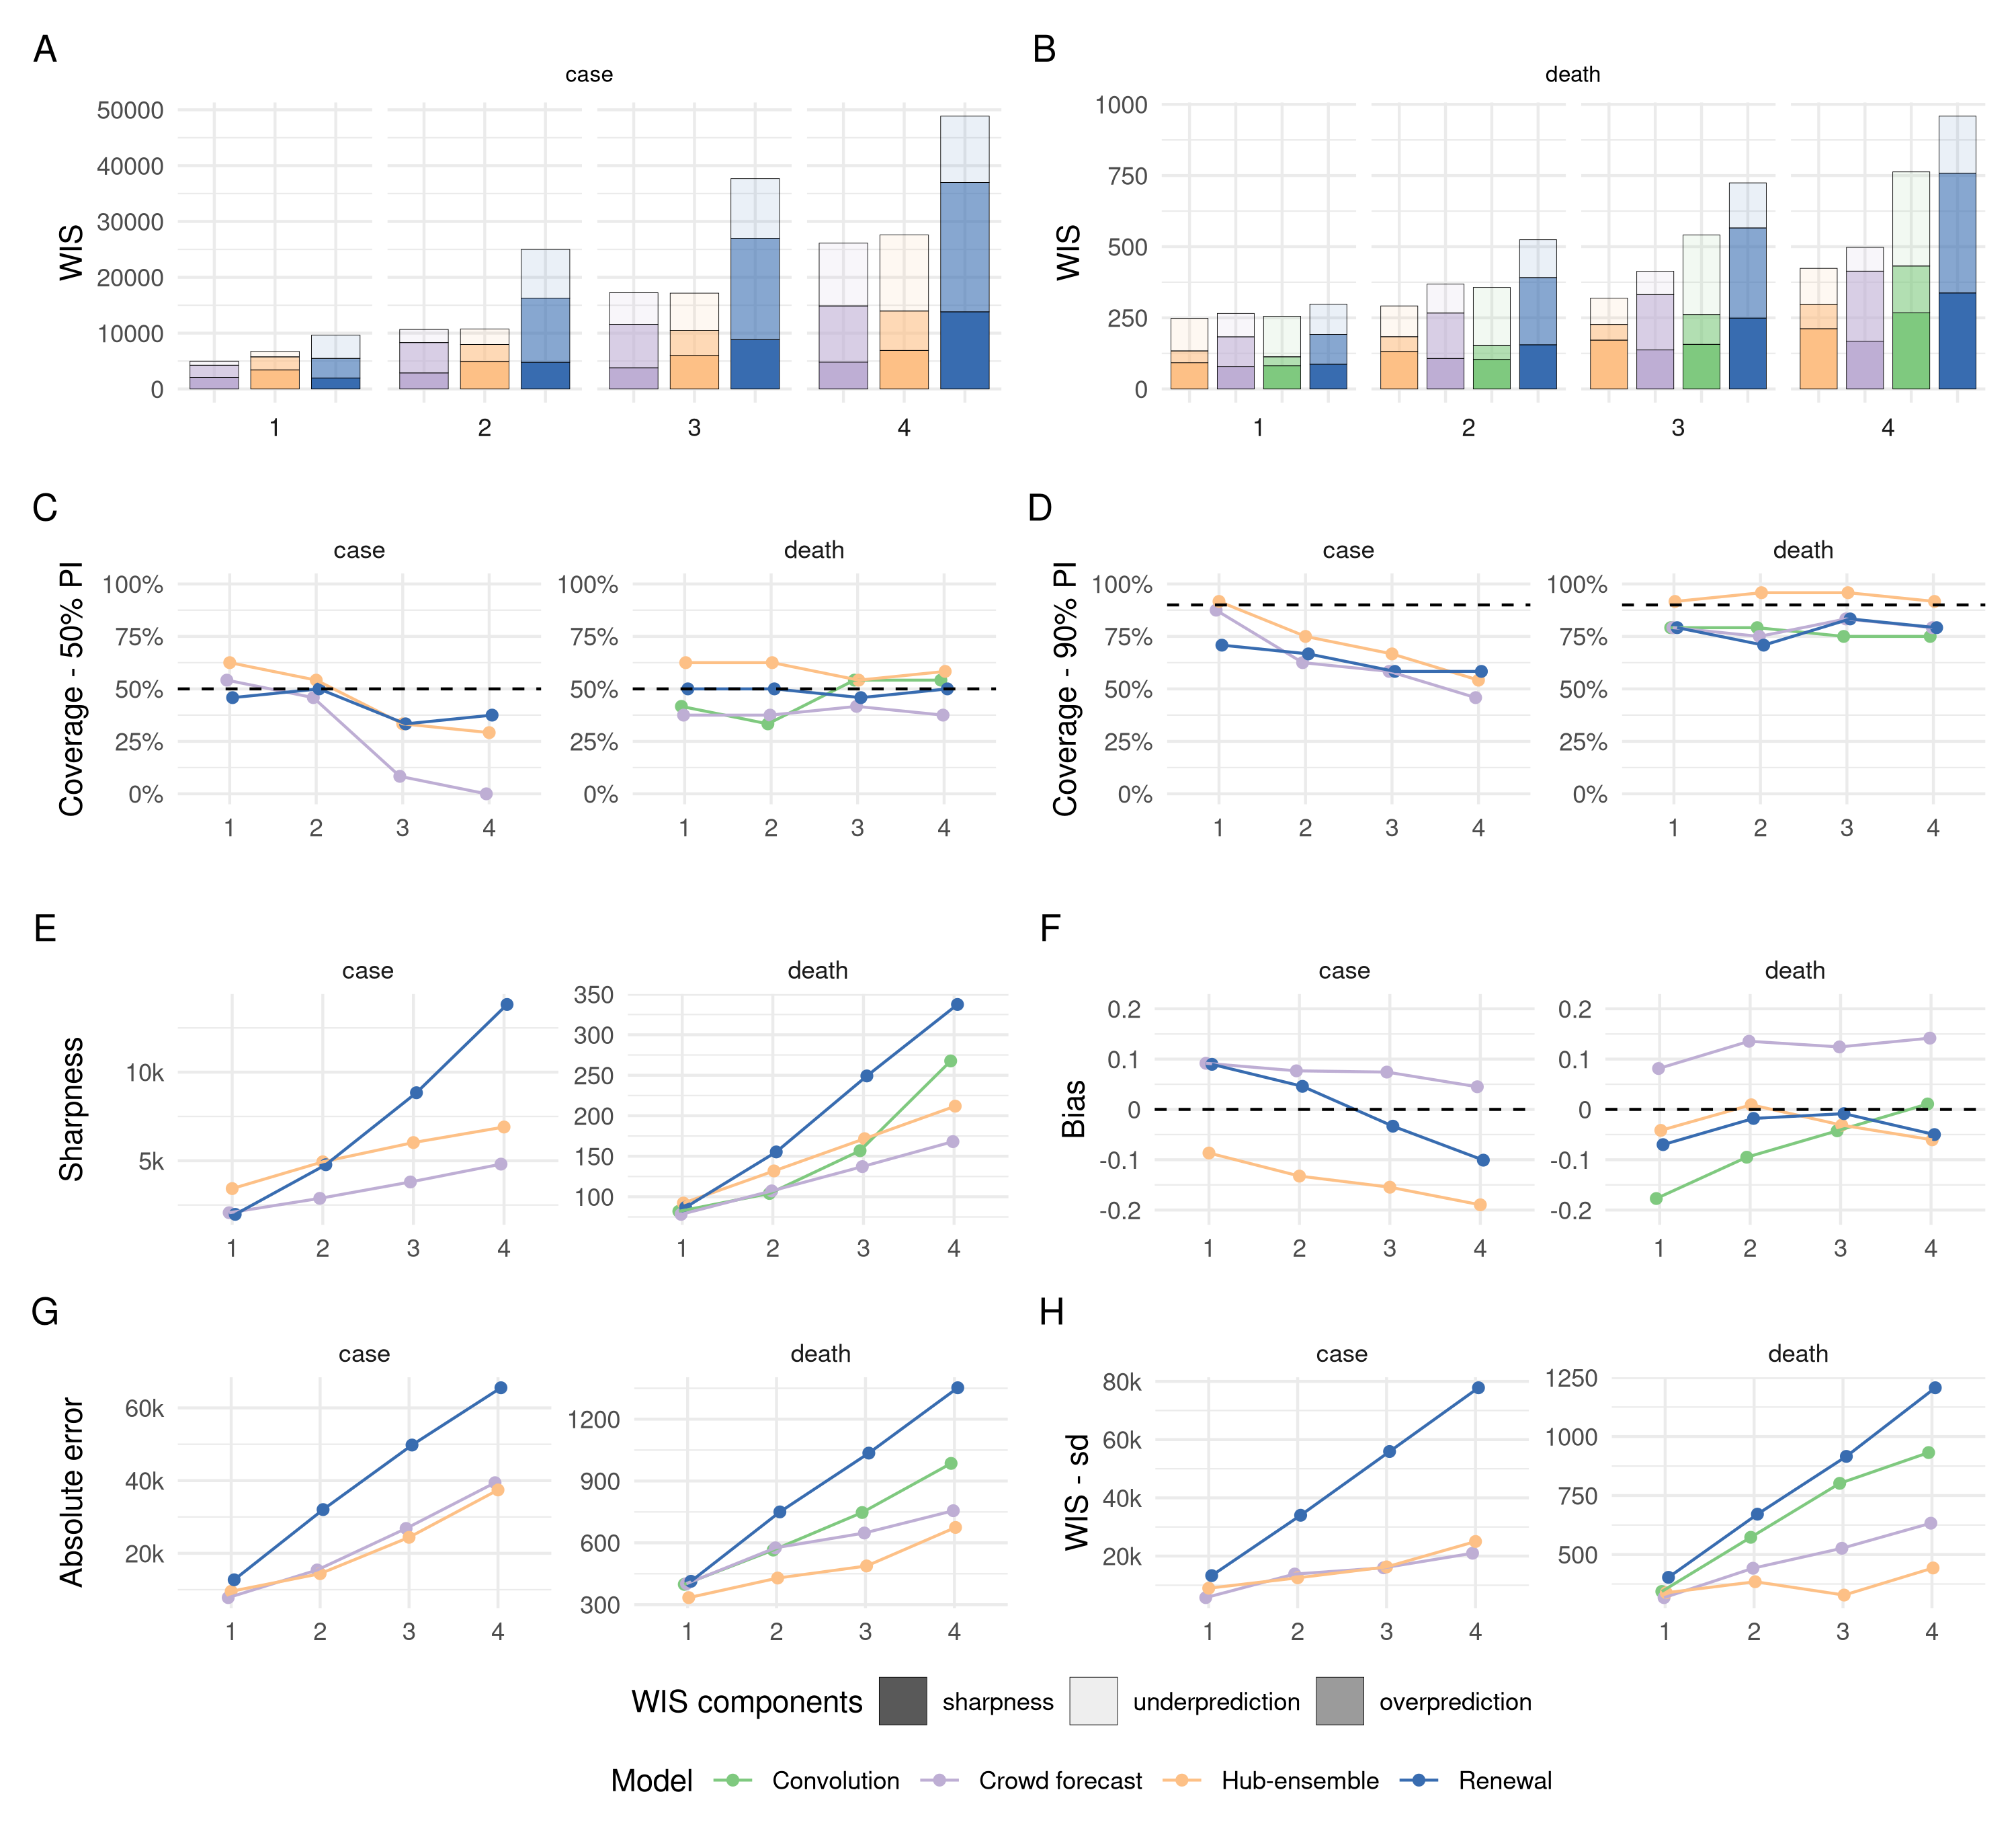
\includegraphics[width=1\linewidth,]{../analysis/plots/aggregate-performance-all-late-period-v4} \caption{Visualisation of aggregate performance metrics across forecast horizons only for the period from October 14th 2020 on where all models were available. A, B: mean weighted interval score (WIS, lower indicates better performance) across horizons. WIS is decomposed into its components dispersion, over-prediction and under-prediction. C: Empirical coverage of the 50\% prediction intervals (50\% coverage is perfect). D: Empirical coverage of the 90\% prediction intervals. E: Dispersion (same as in panel A, B). Higher values mean greater dispersion of the forecast and imply ceteris paribus a worse score. F: Bias, i.e. general (relative) tendency to over- or underpredict. Values are between -1 (complete under-prediction) and 1 (complete over-prediction) and 0 ideally. G: Absolute error of the median forecast (lower is better). H. Standard deviation of all WIS values for different horizons}\label{fig:agg-performance-all-late}
\end{figure}

\begin{table}[!h]
\caption{\label{tab:score-table-late-2}Scores for one and two week ahead forecasts (cut to three significant digits and rounded) calculated on forecasts made between December 14th 2020 and March 1st 2021. Numbers in brackets show the metrics relative to the Hub ensemble (i.e. the median ensemble of all other models submitted to the German and Polish Forecast Hub, excluding our contributions). WIS is the mean weighted interval score (lower values are better), WIS - sd is the standard deviation of all scores achieved by a model. Dispersion, over-prediction and under-prediction together sum up to the weighted interval score. Bias (between -1 and 1, 0 is ideal) represents the general average tendency of a model to over- or underpredict. 50\% and 90\%-coverage are the percentage of observed values that fell within the 50\% and 90\% prediction intervals of a model.\\\hspace{\textwidth}}

\centering
\resizebox{\linewidth}{!}{
\begin{tabular}{>{}llccccccccc}
\toprule
  & Model & WIS & WIS - sd & dispersion & Underpred. & Overpred. & Bias & Abs. error & 50\%-Cov. & 90\%-Cov.\\
\midrule
\addlinespace[0.3em]
\multicolumn{11}{l}{\textbf{Cases}}\\
\hline
\cellcolor{white}{} & Crowd forecast & 4980 (0.74) & 5730 (0.64) & 2070 (0.6) & 728 (0.74) & 2190 (0.94) & 0.09 & 7810 (0.82) & 0.54 & 0.88\\
\cmidrule{2-11}
\cellcolor{white}{} & Hub-ensemble & 6730 (1) & 8960 (1) & 3430 (1) & 978 (1) & 2330 (1) & -0.09 & 9550 (1) & 0.62 & 0.92\\
\cmidrule{2-11}
\cellcolor{white}{\multirow{-3}{*}{\raggedright\arraybackslash 1 wk ahead}} & Renewal & 9640 (1.43) & 13300 (1.48) & 1970 (0.57) & 4170 (4.26) & 3500 (1.5) & 0.09 & 12700 (1.33) & 0.46 & 0.71\\
\cmidrule{1-11}
\cellcolor{white}{} & Crowd forecast & 10700 (0.99) & 13800 (1.1) & 2880 (0.58) & 2350 (0.85) & 5430 (1.79) & 0.08 & 15400 (1.07) & 0.46 & 0.62\\
\cmidrule{2-11}
\cellcolor{white}{} & Hub-ensemble & 10800 (1) & 12500 (1) & 4940 (1) & 2780 (1) & 3030 (1) & -0.13 & 14400 (1) & 0.54 & 0.75\\
\cmidrule{2-11}
\cellcolor{white}{\multirow{-3}{*}{\raggedright\arraybackslash 2 wk ahead}} & Renewal & 25000 (2.31) & 34000 (2.72) & 4780 (0.97) & 8710 (3.13) & 11500 (3.8) & 0.05 & 32000 (2.22) & 0.50 & 0.67\\
\cmidrule{1-11}
\addlinespace[0.3em]
\multicolumn{11}{l}{\textbf{Deaths}}\\
\hline
\cellcolor{white}{} & Convolution & 255 (1.03) & 343 (1.01) & 82 (0.89) & 142 (1.23) & 31.1 (0.75) & -0.18 & 399 (1.19) & 0.42 & 0.79\\
\cmidrule{2-11}
\cellcolor{white}{} & Crowd forecast & 265 (1.07) & 317 (0.94) & 78.2 (0.85) & 82 (0.71) & 105 (2.52) & 0.08 & 402 (1.2) & 0.38 & 0.79\\
\cmidrule{2-11}
\cellcolor{white}{} & Hub-ensemble & 248 (1) & 338 (1) & 92.2 (1) & 115 (1) & 41.6 (1) & -0.04 & 334 (1) & 0.62 & 0.92\\
\cmidrule{2-11}
\cellcolor{white}{\multirow{-4}{*}{\raggedright\arraybackslash 1 wk ahead}} & Renewal & 298 (1.2) & 403 (1.19) & 87 (0.94) & 107 (0.93) & 105 (2.52) & -0.07 & 413 (1.24) & 0.50 & 0.79\\
\cmidrule{1-11}
\cellcolor{white}{} & Convolution & 357 (1.22) & 573 (1.49) & 104 (0.79) & 204 (1.89) & 48.8 (0.94) & -0.10 & 565 (1.32) & 0.33 & 0.79\\
\cmidrule{2-11}
\cellcolor{white}{} & Crowd forecast & 368 (1.26) & 442 (1.15) & 107 (0.81) & 102 (0.94) & 160 (3.08) & 0.14 & 576 (1.34) & 0.38 & 0.75\\
\cmidrule{2-11}
\cellcolor{white}{} & Hub-ensemble & 292 (1) & 385 (1) & 132 (1) & 108 (1) & 51.9 (1) & 0.01 & 429 (1) & 0.62 & 0.96\\
\cmidrule{2-11}
\cellcolor{white}{\multirow{-4}{*}{\raggedright\arraybackslash 2 wk ahead}} & Renewal & 524 (1.79) & 671 (1.74) & 155 (1.17) & 133 (1.23) & 236 (4.55) & -0.02 & 750 (1.75) & 0.50 & 0.71\\
\bottomrule
\end{tabular}}
\end{table}

\begin{table}[!h]
\caption{\label{tab:score-table-late-4}Scores for three and four week ahead forecasts (cut to three significant digits and rounded) calculated on forecasts made between December 14th 2020 and March 1st 2021. Numbers in brackets show the metrics relative to the Hub ensemble (i.e. the median ensemble of all other models submitted to the German and Polish Forecast Hub, excluding our contributions). WIS is the mean weighted interval score (lower values are better), WIS - sd is the standard deviation of all scores achieved by a model. Dispersion, over-prediction and under-prediction together sum up to the weighted interval score. Bias (between -1 and 1, 0 is ideal) represents the general average tendency of a model to over- or underpredict. 50\% and 90\%-coverage are the percentage of observed values that fell within the 50\% and 90\% prediction intervals of a model.\\\hspace{\textwidth}}

\centering
\resizebox{\linewidth}{!}{
\begin{tabular}{>{}llccccccccc}
\toprule
  & Model & WIS & WIS - sd & dispersion & Underpred. & Overpred. & Bias & Abs. error & 50\%-Cov. & 90\%-Cov.\\
\midrule
\addlinespace[0.3em]
\multicolumn{11}{l}{\textbf{Cases}}\\
\hline
\cellcolor{white}{} & Crowd forecast & 17200 (1) & 16000 (0.98) & 3800 (0.63) & 5660 (0.85) & 7770 (1.74) & 0.07 & 26800 (1.1) & 0.08 & 0.58\\
\cmidrule{2-11}
\cellcolor{white}{} & Hub-ensemble & 17200 (1) & 16300 (1) & 6030 (1) & 6670 (1) & 4470 (1) & -0.16 & 24400 (1) & 0.33 & 0.67\\
\cmidrule{2-11}
\cellcolor{white}{\multirow{-3}{*}{\raggedright\arraybackslash 3 wk ahead}} & Renewal & 37700 (2.19) & 55900 (3.43) & 8840 (1.47) & 10700 (1.6) & 18100 (4.05) & -0.03 & 49800 (2.04) & 0.33 & 0.58\\
\cmidrule{1-11}
\cellcolor{white}{} & Crowd forecast & 26100 (0.95) & 21000 (0.84) & 4810 (0.7) & 11300 (0.83) & 10100 (1.43) & 0.04 & 39400 (1.05) & 0.00 & 0.46\\
\cmidrule{2-11}
\cellcolor{white}{} & Hub-ensemble & 27600 (1) & 25000 (1) & 6900 (1) & 13600 (1) & 7060 (1) & -0.19 & 37400 (1) & 0.29 & 0.54\\
\cmidrule{2-11}
\cellcolor{white}{\multirow{-3}{*}{\raggedright\arraybackslash 4 wk ahead}} & Renewal & 48900 (1.77) & 77800 (3.11) & 13800 (2) & 11900 (0.88) & 23200 (3.29) & -0.10 & 65500 (1.75) & 0.38 & 0.58\\
\cmidrule{1-11}
\addlinespace[0.3em]
\multicolumn{11}{l}{\textbf{Deaths}}\\
\hline
\cellcolor{white}{} & Convolution & 541 (1.7) & 802 (2.45) & 157 (0.91) & 279 (3.01) & 105 (1.91) & -0.04 & 747 (1.53) & 0.54 & 0.75\\
\cmidrule{2-11}
\cellcolor{white}{} & Crowd forecast & 414 (1.3) & 526 (1.6) & 137 (0.8) & 82 (0.88) & 194 (3.52) & 0.12 & 648 (1.33) & 0.42 & 0.83\\
\cmidrule{2-11}
\cellcolor{white}{} & Hub-ensemble & 319 (1) & 328 (1) & 172 (1) & 92.7 (1) & 55.1 (1) & -0.03 & 488 (1) & 0.54 & 0.96\\
\cmidrule{2-11}
\cellcolor{white}{\multirow{-4}{*}{\raggedright\arraybackslash 3 wk ahead}} & Renewal & 724 (2.27) & 916 (2.79) & 249 (1.45) & 158 (1.7) & 317 (5.75) & -0.01 & 1040 (2.13) & 0.46 & 0.83\\
\cmidrule{1-11}
\cellcolor{white}{} & Convolution & 763 (1.8) & 932 (2.1) & 268 (1.26) & 331 (2.63) & 164 (1.91) & 0.01 & 985 (1.46) & 0.54 & 0.75\\
\cmidrule{2-11}
\cellcolor{white}{} & Crowd forecast & 498 (1.17) & 633 (1.43) & 168 (0.79) & 83.6 (0.66) & 246 (2.87) & 0.14 & 756 (1.12) & 0.38 & 0.79\\
\cmidrule{2-11}
\cellcolor{white}{} & Hub-ensemble & 424 (1) & 443 (1) & 212 (1) & 126 (1) & 85.7 (1) & -0.06 & 675 (1) & 0.58 & 0.92\\
\cmidrule{2-11}
\cellcolor{white}{\multirow{-4}{*}{\raggedright\arraybackslash 4 wk ahead}} & Renewal & 959 (2.26) & 1210 (2.73) & 337 (1.59) & 200 (1.59) & 421 (4.91) & -0.05 & 1350 (2) & 0.50 & 0.79\\
\bottomrule
\end{tabular}}
\end{table}

\clearpage

\hypertarget{overview-of-models-and-forecasters}{%
\subsection{Overview of models and forecasters}\label{overview-of-models-and-forecasters}}

\begin{longtable}[t]{>{\raggedright\arraybackslash}p{4.5cm}>{\raggedright\arraybackslash}p{11.0cm}}
\caption{\label{tab:table-ensemble-versions}Overview of the models and ensembles used.}\\
\toprule
Name & Explanation\\
\midrule
\endfirsthead
\caption[]{\label{tab:table-ensemble-versions}Overview of the models and ensembles used. \textit{(continued)}}\\
\toprule
Name & Explanation\\
\midrule
\endhead

\endfoot
\bottomrule
\endlastfoot
\cellcolor{gray!6}{Hub-ensemble-realised} & \cellcolor{gray!6}{Official Forecast Hub median ensemble. Created by the Forecast Hub officially under the name 'KITCOVIDhub-median\_ensemble' and used as the default ensemble. Included are our crowd forecasts as well as the renewal model (with one missed submission on December 28 2020, but not the convolution model which was deemed to similar to the renewal model.}\\
\addlinespace \addlinespace
Hub-ensemble-realised-mean & Official Forecast Hub mean ensemble. Created by the Forecast Hub officially under the name 'KITCOVIDhub-mean\_ensemble'.\\
\addlinespace \addlinespace
\cellcolor{gray!6}{ \vphantom{1}} & \cellcolor{gray!6}{}\\
\addlinespace \addlinespace
Hub-ensemble & Version of the official Hub median ensemble which excludes all our contributions.\\
\addlinespace \addlinespace
\cellcolor{gray!6}{Hub-ensemble-mean} & \cellcolor{gray!6}{Version of the official Hub mean ensemble which excludes all our contributions.}\\
\addlinespace \addlinespace
Hub-ensemble-with-renewal, 
    Hub-ensemble-with-renewal-mean & Versions of the official Hub ensembles which of our contributions includes only the Renewal model.\\
\addlinespace \addlinespace
Hub-ensemble-with-crowd, 
\cellcolor{gray!6}{    Hub-ensemble-with-crowd-mean} & \cellcolor{gray!6}{Versions of the official Hub ensembles which of our contributions includes only the Crowd forecast.}\\
\addlinespace \addlinespace
Hub-ensemble-with-convolution, 
    Hub-ensemble-with-convolution-mean & Versions of the official Hub ensembles which of our contributions includes only the Convolution model (which originally was never included in any official Hub ensemble).\\
\addlinespace \addlinespace
Hub-ensemble-with-all, 
\cellcolor{gray!6}{    Hub-ensemble-with-all-mean} & \cellcolor{gray!6}{Versions of the official Hub ensembles which includes all our contributions. For cases, this is identical to the official Hub ensembles, but for deaths the convolution model was added.}\\
\addlinespace \addlinespace
 & \\
\addlinespace \addlinespace
\cellcolor{gray!6}{Crowd forecast} & \cellcolor{gray!6}{Submitted to the Forecast Hub as 'epiforecasts-EpiExpert'}\\
\addlinespace \addlinespace
Renewal model & Submitted to the Forecast Hub as 'epiforecasts-EpiNow2'\\
\addlinespace \addlinespace
\cellcolor{gray!6}{Convolution model} & \cellcolor{gray!6}{Submitted to the Forecast Hub as 'epiforecasts-EpiNow2\_secondary'}\\*
\end{longtable}

\begin{figure}[H]
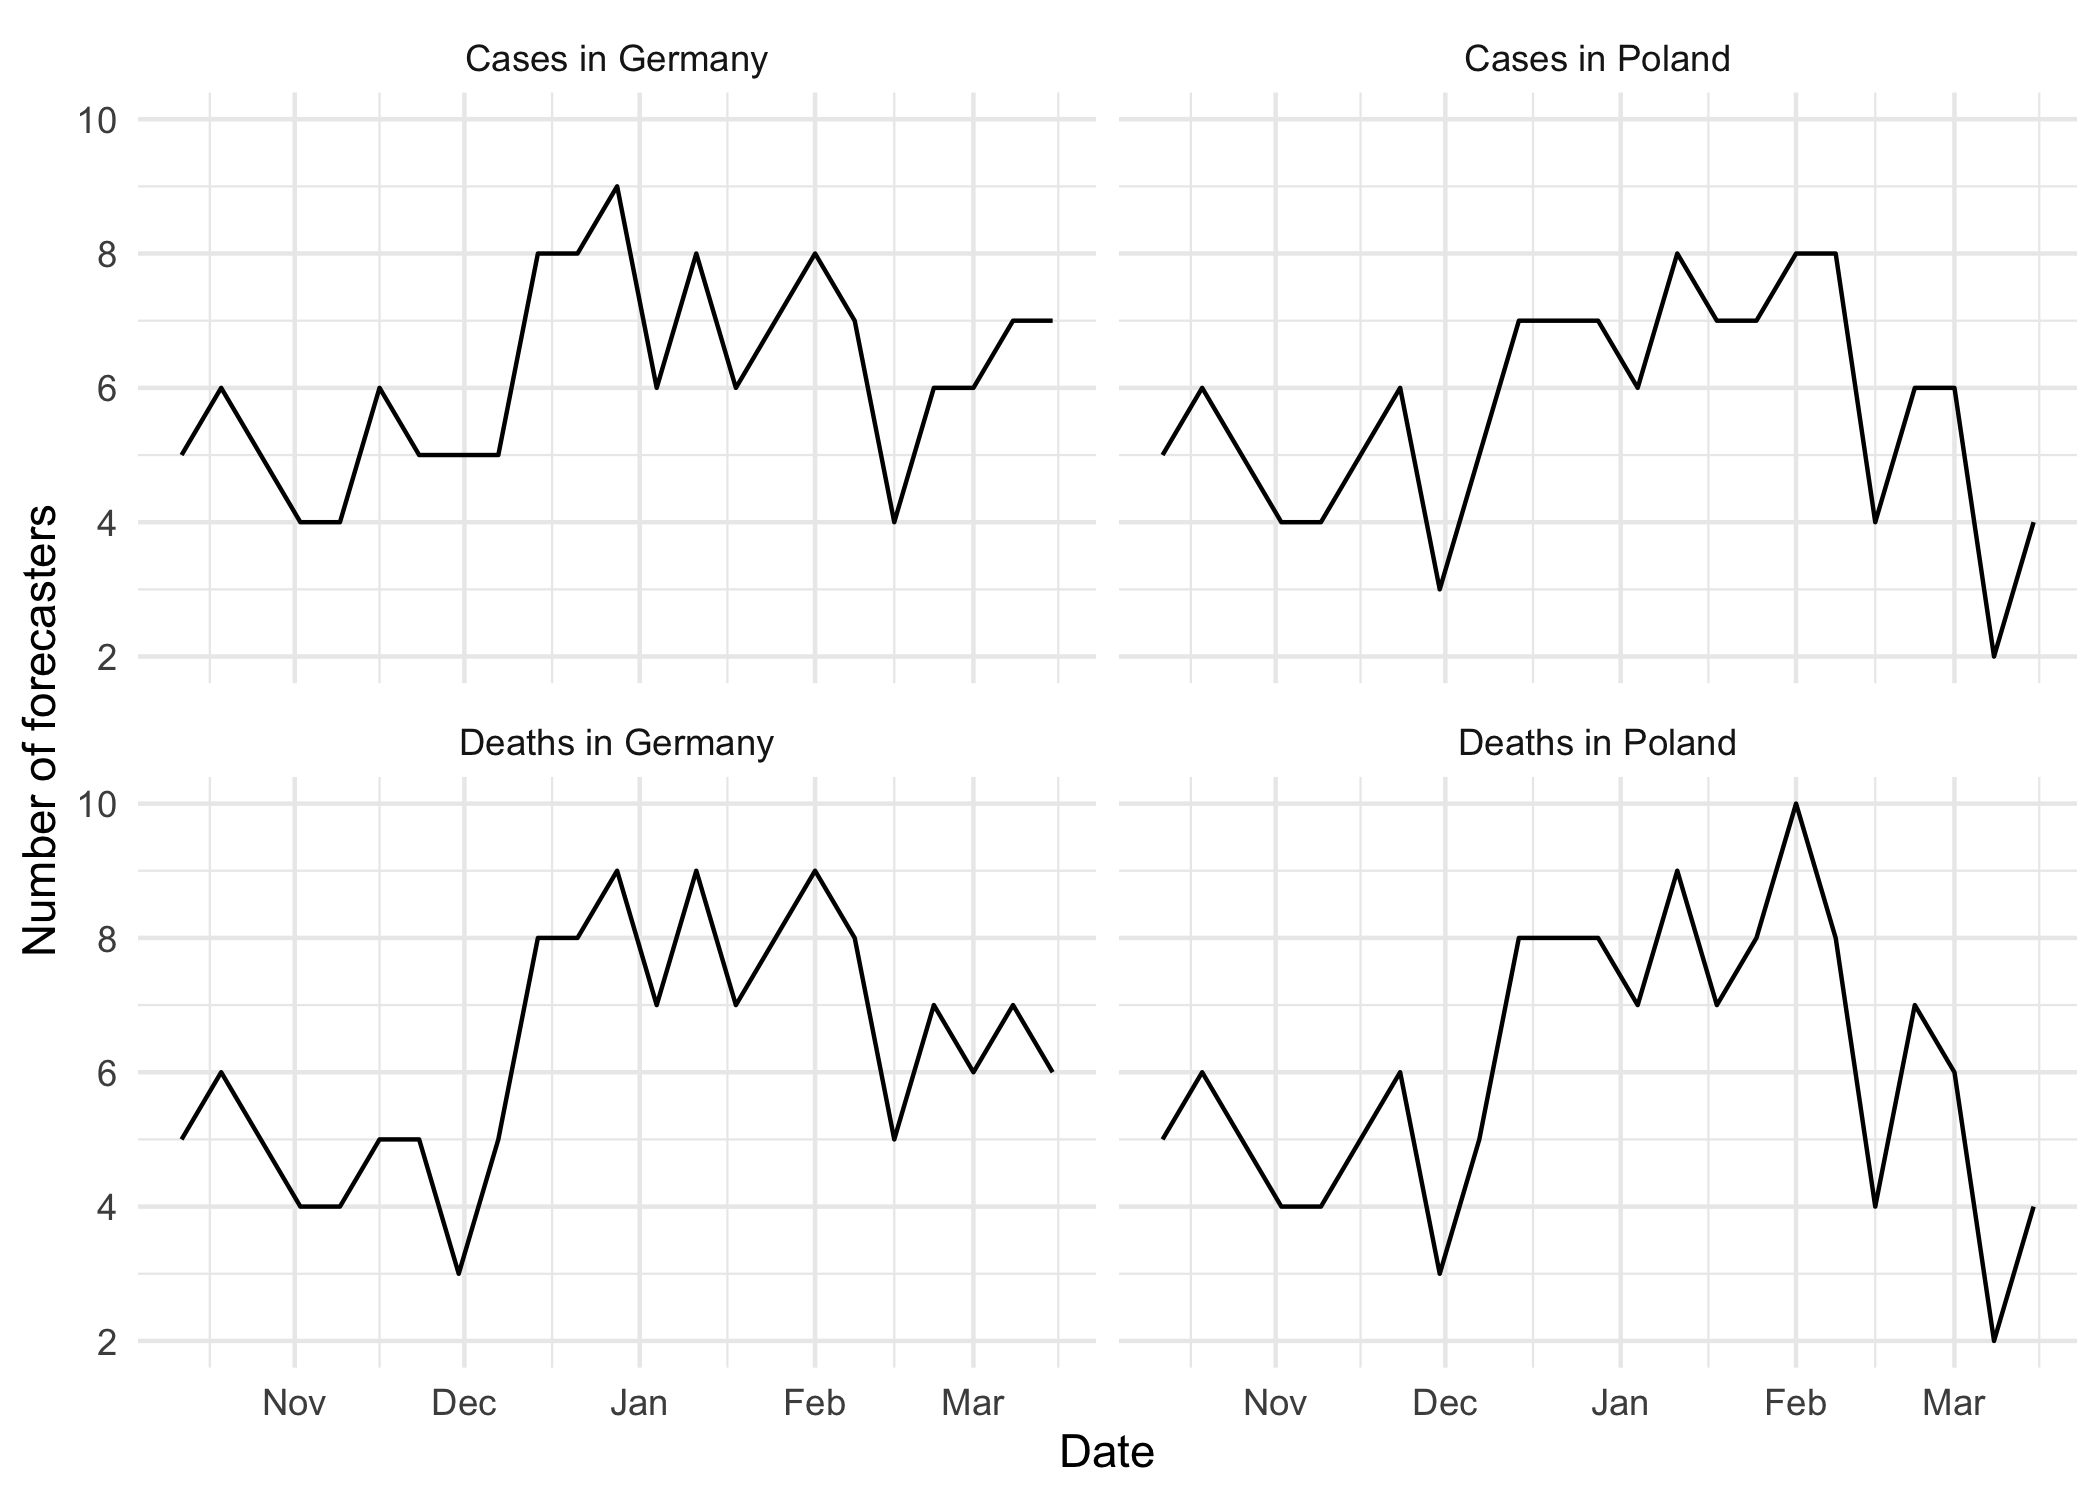
\includegraphics[width=1\linewidth,]{../analysis/plots/number-forecasters} \caption{Number of participants who submitted a forecast over time.}\label{fig:num-forecasters}
\end{figure}

\begin{figure}[H]
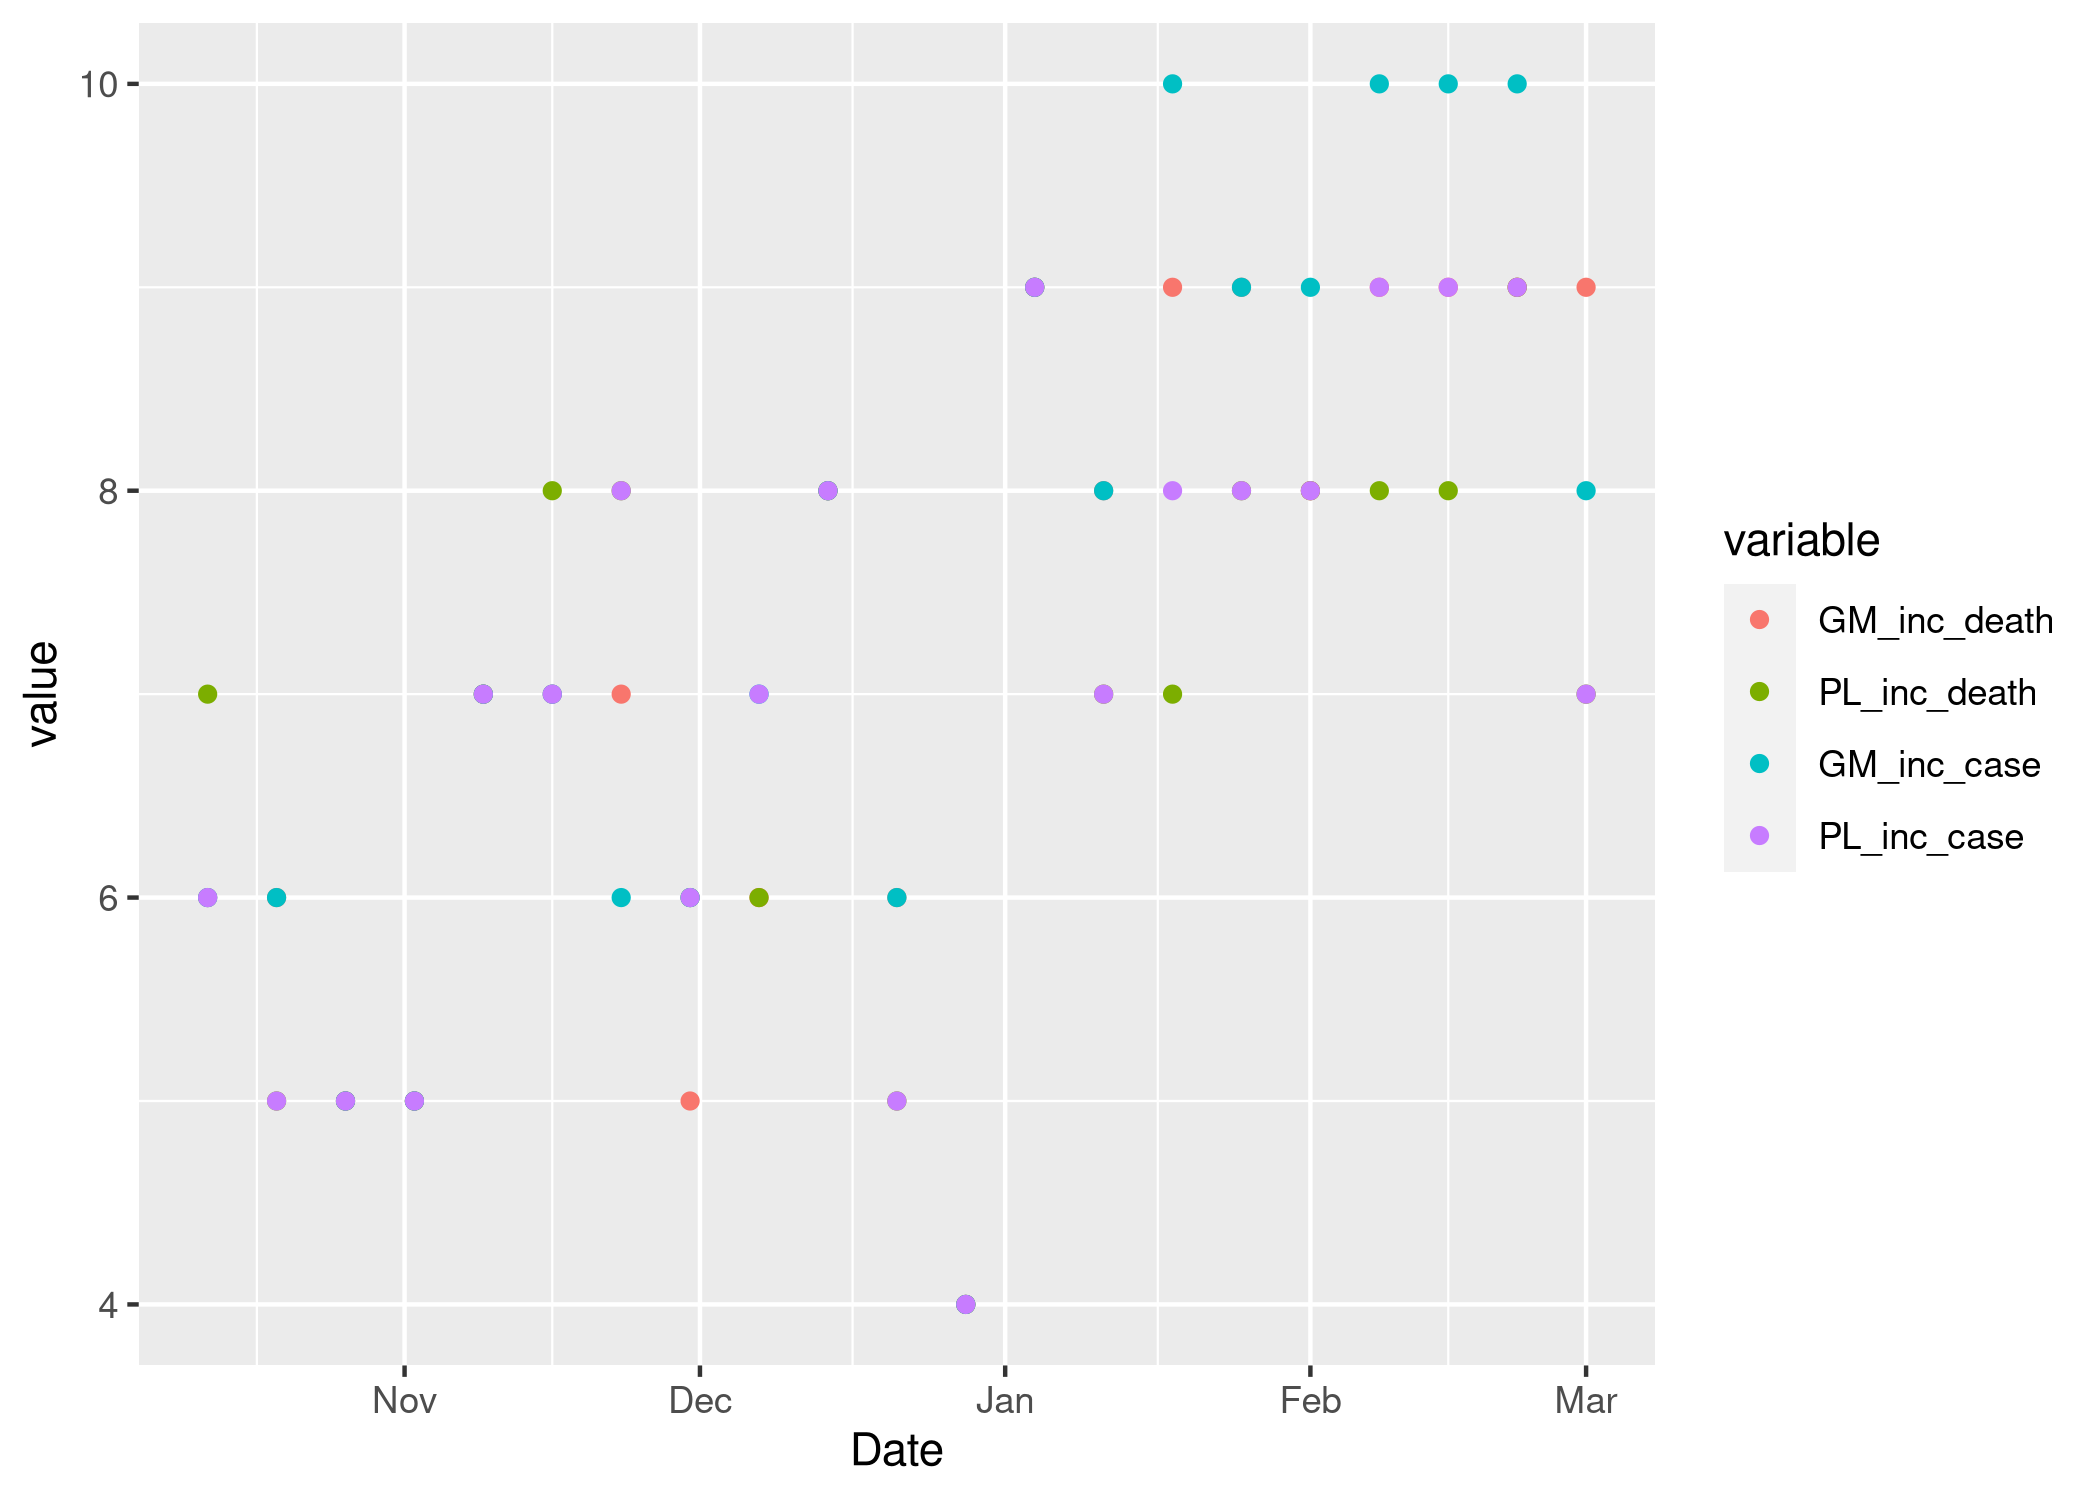
\includegraphics[width=1\linewidth,]{../analysis/plots/ensemble-members} \caption{Number of member models (including our crowd forecasts and the renewal model) in the official Hub ensemble. Note that the renewal model was not included in the ensemble on December 28th 2020.}\label{fig:num-ensemble-members}
\end{figure}

\clearpage

\hypertarget{refs}{}
\begin{CSLReferences}{1}{0}
\leavevmode\vadjust pre{\hypertarget{ref-epinow2}{}}%
Abbott, Sam, Joel Hellewell, Joe Hickson, James Munday, Katelyn Gostic, Peter Ellis, Katharine Sherratt, et al. 2020. {``EpiNow2: Estimate Real-Time Case Counts and Time-Varying Epidemiological Parameters.''} \emph{-} - (-): --. \url{https://doi.org/10.5281/zenodo.3957489}.

\leavevmode\vadjust pre{\hypertarget{ref-covidregionaldata}{}}%
Abbott, Sam, Katharine Sherratt, Jonnie Bevan, Hamish Gibbs, Joel Hellewell, James Munday, Patrick Barks, Paul Campbell, Flavio Finger, and Sebastian Funk. 2020. {``Covidregionaldata: Subnational Data for the Covid-19 Outbreak.''} \emph{-} - (-): --. \url{https://doi.org/10.5281/zenodo.3957539}.

\leavevmode\vadjust pre{\hypertarget{ref-aerzteblattSARSCoV2DiagnostikRKIPasst2020}{}}%
Ärzteblatt, Deutscher Ärzteverlag GmbH, Redaktion Deutsches. 2020. {``SARS-CoV-2-Diagnostik: RKI passt Testempfehlungen an.''} {Deutsches Ärzteblatt}. November 3, 2020. \url{https://www.aerzteblatt.de/nachrichten/118001/SARS-CoV-2-Diagnostik-RKI-passt-Testempfehlungen-an}.

\leavevmode\vadjust pre{\hypertarget{ref-atanasovDistillingWisdomCrowds2016}{}}%
Atanasov, Pavel, Phillip Rescober, Eric Stone, Samuel A. Swift, Emile Servan-Schreiber, Philip Tetlock, Lyle Ungar, and Barbara Mellers. 2016. {``Distilling the {Wisdom} of {Crowds}: Prediction {Markets} Vs. {Prediction Polls}.''} \emph{Management Science} 63 (3): 691--706. \url{https://doi.org/10.1287/mnsc.2015.2374}.

\leavevmode\vadjust pre{\hypertarget{ref-bhattSemiMechanisticBayesianModeling}{}}%
Bhatt, Samir, Neil Ferguson, Seth Flaxman, Axel Gandy, Swapnil Mishra, and James A Scott. n.d. {``Semi-{Mechanistic Bayesian} Modeling of {COVID}-19 with {Renewal Processes},''} 14.

\leavevmode\vadjust pre{\hypertarget{ref-biggerstaffResultsCentersDisease2016}{}}%
Biggerstaff, Matthew, David Alper, Mark Dredze, Spencer Fox, Isaac Chun-Hai Fung, Kyle S. Hickmann, Bryan Lewis, et al. 2016. {``Results from the Centers for Disease Control and Prevention's Predict the 2013--2014 {Influenza Season Challenge}.''} \emph{BMC Infectious Diseases} 16 (1): 357. \url{https://doi.org/10.1186/s12879-016-1669-x}.

\leavevmode\vadjust pre{\hypertarget{ref-crowdforecastr}{}}%
Bosse, Nikos I., Sam Abbott, EpiForecasts, and Sebastian Funk. 2020. \emph{Crowdforecastr: Eliciting Crowd Forecasts in r Shiny}. \url{https://doi.org/10.5281/zenodo.4618519}.

\leavevmode\vadjust pre{\hypertarget{ref-covidgermanforecasts}{}}%
Bosse, Nikos, Sam Abbott, EpiForecasts, and Sebastian Funk. 2020. \emph{Covid.german.forecasts: Forecasting Covid-19 Related Metrics for the German/Poland Forecast Hub}.

\leavevmode\vadjust pre{\hypertarget{ref-bracherEvaluatingEpidemicForecasts2021}{}}%
Bracher, Johannes, Evan L. Ray, Tilmann Gneiting, and Nicholas G. Reich. 2021. {``Evaluating Epidemic Forecasts in an Interval Format.''} \emph{PLoS Computational Biology} 17 (2): e1008618. \url{https://doi.org/10.1371/journal.pcbi.1008618}.

\leavevmode\vadjust pre{\hypertarget{ref-bracherShorttermForecastingCOVID192021}{}}%
Bracher, Johannes, Daniel Wolffram, J. Deuschel, K. Görgen, J. L. Ketterer, A. Ullrich, S. Abbott, et al. 2021. {``Short-Term Forecasting of {COVID}-19 in {Germany} and {Poland} During the Second Wave -- a Preregistered Study.''} \emph{medRxiv}, January, 2020.12.24.20248826. \url{https://doi.org/10.1101/2020.12.24.20248826}.

\leavevmode\vadjust pre{\hypertarget{ref-shiny}{}}%
Chang, Winston, Joe Cheng, JJ Allaire, Carson Sievert, Barret Schloerke, Yihui Xie, Jeff Allen, Jonathan McPherson, Alan Dipert, and Barbara Borges. 2021. \emph{Shiny: Web Application Framework for r}. \url{https://CRAN.R-project.org/package=shiny}.

\leavevmode\vadjust pre{\hypertarget{ref-colon-gonzalezProbabilisticSeasonalDengue2021}{}}%
Colón-González, Felipe J., Leonardo Soares Bastos, Barbara Hofmann, Alison Hopkin, Quillon Harpham, Tom Crocker, Rosanna Amato, et al. 2021. {``Probabilistic Seasonal Dengue Forecasting in {Vietnam}: A Modelling Study Using Superensembles.''} \emph{PLOS Medicine} 18 (3): e1003542. \url{https://doi.org/10.1371/journal.pmed.1003542}.

\leavevmode\vadjust pre{\hypertarget{ref-COVID19DataExplorer}{}}%
{``{COVID}-19 {Data Explorer}.''} n.d. {Our World in Data}. Accessed May 30, 2021. \url{https://ourworldindata.org/coronavirus-data-explorer}.

\leavevmode\vadjust pre{\hypertarget{ref-cramerEvaluationIndividualEnsemble2021}{}}%
Cramer, Estee, Evan L. Ray, Velma K. Lopez, Johannes Bracher, Andrea Brennen, Alvaro J. Castro Rivadeneira, Aaron Gerding, et al. 2021. {``Evaluation of Individual and Ensemble Probabilistic Forecasts of {COVID}-19 Mortality in the {US}.''} \emph{medRxiv}, February, 2021.02.03.21250974. \url{https://doi.org/10.1101/2021.02.03.21250974}.

\leavevmode\vadjust pre{\hypertarget{ref-cramerCOVID19ForecastHub2020}{}}%
Cramer, Estee, Nicholas G Reich, Serena Yijin Wang, Jarad Niemi, Abdul Hannan, Katie House, Youyang Gu, et al. 2020. {``{COVID}-19 {Forecast Hub}: 4 {December} 2020 Snapshot.''} {Zenodo}. \url{https://doi.org/10.5281/zenodo.3963371}.

\leavevmode\vadjust pre{\hypertarget{ref-CSETForetell}{}}%
{``{CSET Foretell}.''} n.d. Accessed October 13, 2021. \url{https://www.cset-foretell.com/}.

\leavevmode\vadjust pre{\hypertarget{ref-delvalleSummaryResults201420152018}{}}%
Del Valle, Sara Y., Benjamin H. McMahon, Jason Asher, Richard Hatchett, Joceline C. Lega, Heidi E. Brown, Mark E. Leany, et al. 2018. {``Summary Results of the 2014-2015 {DARPA Chikungunya} Challenge.''} \emph{BMC Infectious Diseases} 18 (1): 245. \url{https://doi.org/10.1186/s12879-018-3124-7}.

\leavevmode\vadjust pre{\hypertarget{ref-doiCovid19TemporalVariation}{}}%
DOI, Authors Affiliations Published Not published yet. n.d. {``Covid-19: Temporal Variation in Transmission During the {COVID}-19 Outbreak.''} {Covid-19}. Accessed May 30, 2021. \url{https://epiforecasts.io/covid/}.

\leavevmode\vadjust pre{\hypertarget{ref-DownloadHistoricalData2020a}{}}%
{``Download Historical Data (to 14 {December} 2020) on the Daily Number of New Reported {COVID}-19 Cases and Deaths Worldwide.''} 2020. {European Centre for Disease Prevention and Control}. December 14, 2020. \url{https://www.ecdc.europa.eu/en/publications-data/download-todays-data-geographic-distribution-covid-19-cases-worldwide}.

\leavevmode\vadjust pre{\hypertarget{ref-EvaluatingUseReproduction}{}}%
{``Evaluating the Use of the Reproduction Number as an Epidemiological Tool, Using Spatio-Temporal Trends of the {Covid}-19 Outbreak in {England} \textbar{} {medRxiv}.''} n.d. Accessed May 30, 2021. \url{https://www.medrxiv.org/content/10.1101/2020.10.18.20214585v1}.

\leavevmode\vadjust pre{\hypertarget{ref-farrowHumanJudgmentApproach2017}{}}%
Farrow, David C., Logan C. Brooks, Sangwon Hyun, Ryan J. Tibshirani, Donald S. Burke, and Roni Rosenfeld. 2017. {``A Human Judgment Approach to Epidemiological Forecasting.''} \emph{PLOS Computational Biology} 13 (3): e1005248. \url{https://doi.org/10.1371/journal.pcbi.1005248}.

\leavevmode\vadjust pre{\hypertarget{ref-golem}{}}%
Fay, Colin, Vincent Guyader, Sébastien Rochette, and Cervan Girard. 2021. \emph{Golem: A Framework for Robust Shiny Applications}. \url{https://github.com/ThinkR-open/golem}.

\leavevmode\vadjust pre{\hypertarget{ref-fraserEstimatingIndividualHousehold2007}{}}%
Fraser, Christophe. 2007. {``Estimating {Individual} and {Household Reproduction Numbers} in an {Emerging Epidemic}.''} \emph{PLOS ONE} 2 (8): e758. \url{https://doi.org/10.1371/journal.pone.0000758}.

\leavevmode\vadjust pre{\hypertarget{ref-funkShorttermForecastsInform2020}{}}%
Funk, Sebastian, Sam Abbott, B. D. Atkins, M. Baguelin, J. K. Baillie, P. Birrell, J. Blake, et al. 2020. {``Short-Term Forecasts to Inform the Response to the {Covid}-19 Epidemic in the {UK}.''} \emph{medRxiv}, November, 2020.11.11.20220962. \url{https://doi.org/10.1101/2020.11.11.20220962}.

\leavevmode\vadjust pre{\hypertarget{ref-funkAssessingPerformanceRealtime2019}{}}%
Funk, Sebastian, Anton Camacho, Adam J. Kucharski, Rachel Lowe, Rosalind M. Eggo, and W. John Edmunds. 2019. {``Assessing the Performance of Real-Time Epidemic Forecasts: A Case Study of {Ebola} in the {Western Area} Region of {Sierra Leone}, 2014-15.''} \emph{PLOS Computational Biology} 15 (2): e1006785. \url{https://doi.org/10.1371/journal.pcbi.1006785}.

\leavevmode\vadjust pre{\hypertarget{ref-generationinterval}{}}%
Ganyani, Tapiwa, Cecile Kremer, Dongxuan Chen, Andrea Torneri, Christel Faes, Jacco Wallinga, and Niel Hens. 2020. {``Estimating the Generation Interval for Coronavirus Disease (COVID-19) Based on Symptom Onset Data, March 2020.''} \emph{Eurosurveillance} 25 (17).

\leavevmode\vadjust pre{\hypertarget{ref-gneiting_strictly_2007}{}}%
Gneiting, Tilmann, and Adrian E Raftery. 2007. {``Strictly Proper Scoring Rules, Prediction, and Estimation.''} \emph{Journal of the American Statistical Association} 102 (477): 359--78. \url{https://doi.org/10.1198/016214506000001437}.

\leavevmode\vadjust pre{\hypertarget{ref-heldProbabilisticForecastingInfectious2017}{}}%
Held, Leonhard, Sebastian Meyer, and Johannes Bracher. 2017. {``Probabilistic Forecasting in Infectious Disease Epidemiology: The 13th {Armitage} Lecture.''} \emph{Statistics in Medicine} 36 (22): 3443--60. \url{https://doi.org/10.1002/sim.7363}.

\leavevmode\vadjust pre{\hypertarget{ref-hoogeveenLaypeopleCanPredict2020}{}}%
Hoogeveen, Suzanne, Alexandra Sarafoglou, and Eric-Jan Wagenmakers. 2020. {``Laypeople {Can Predict Which Social}-{Science Studies Will Be Replicated Successfully}.''} \emph{Advances in Methods and Practices in Psychological Science} 3 (3): 267--85. \url{https://doi.org/10.1177/2515245920919667}.

\leavevmode\vadjust pre{\hypertarget{ref-EuroHub}{}}%
Hub, European COVID-19 Forecast. 2021. {``Forecasts of New Cases and Deaths Due to Covid-19 over the Next Four Weeks in Countries Across Europe and the UK.''} \url{https://covid19forecasthub.eu/}.

\leavevmode\vadjust pre{\hypertarget{ref-HypermindSupercollectiveIntelligence}{}}%
{``Hypermind \textbar{} {Supercollective} Intelligence for Decision Makers.''} n.d. {Hypermind}. Accessed October 13, 2021. \url{https://www.hypermind.com/en/}.

\leavevmode\vadjust pre{\hypertarget{ref-johanssonOpenChallengeAdvance2019}{}}%
Johansson, Michael A., Karyn M. Apfeldorf, Scott Dobson, Jason Devita, Anna L. Buczak, Benjamin Baugher, Linda J. Moniz, et al. 2019. {``An Open Challenge to Advance Probabilistic Forecasting for Dengue Epidemics.''} \emph{Proceedings of the National Academy of Sciences} 116 (48): 24268--74. \url{https://doi.org/10.1073/pnas.1909865116}.

\leavevmode\vadjust pre{\hypertarget{ref-incubationperiod}{}}%
Lauer, Stephen A, Kyra H Grantz, Qifang Bi, Forrest K Jones, Qulu Zheng, Hannah R Meredith, Andrew S Azman, Nicholas G Reich, and Justin Lessler. 2020. {``The Incubation Period of Coronavirus Disease 2019 (COVID-19) from Publicly Reported Confirmed Cases: Estimation and Application.''} \emph{Annals of Internal Medicine} 172 (9): 577--82.

\leavevmode\vadjust pre{\hypertarget{ref-mcandrewExpertJudgmentModel2020}{}}%
McAndrew, Thomas Charles, and Nicholas G. Reich. 2020. {``An Expert Judgment Model to Predict Early Stages of the {COVID}-19 Outbreak in the {United States}.''} \emph{medRxiv}, September, 2020.09.21.20196725. \url{https://doi.org/10.1101/2020.09.21.20196725}.

\leavevmode\vadjust pre{\hypertarget{ref-mcgowanCollaborativeEffortsForecast2019}{}}%
McGowan, Craig J., Matthew Biggerstaff, Michael Johansson, Karyn M. Apfeldorf, Michal Ben-Nun, Logan Brooks, Matteo Convertino, et al. 2019. {``Collaborative Efforts to Forecast Seasonal Influenza in the {United States}, 2015--2016.''} \emph{Scientific Reports} 9 (1, 1): 683. \url{https://doi.org/10.1038/s41598-018-36361-9}.

\leavevmode\vadjust pre{\hypertarget{ref-metaculusPreliminaryLookMetaculus2020}{}}%
Metaculus. 2020. {``A {Preliminary Look} at {Metaculus} and {Expert Forecasts}.''} June 22, 2020. \url{https://www.metaculus.com/news/2020/06/02/LRT/}.

\leavevmode\vadjust pre{\hypertarget{ref-PredictIt}{}}%
{``{PredictIt}.''} n.d. Accessed October 13, 2021. \url{https://www.predictit.org/}.

\leavevmode\vadjust pre{\hypertarget{ref-recchiaHowWellDid2021}{}}%
Recchia, Gabriel, Alexandra L. J. Freeman, and David Spiegelhalter. 2021. {``How Well Did Experts and Laypeople Forecast the Size of the {COVID}-19 Pandemic?''} \emph{PLOS ONE} 16 (5): e0250935. \url{https://doi.org/10.1371/journal.pone.0250935}.

\leavevmode\vadjust pre{\hypertarget{ref-reichCollaborativeMultiyearMultimodel2019}{}}%
Reich, Nicholas G., Logan C. Brooks, Spencer J. Fox, Sasikiran Kandula, Craig J. McGowan, Evan Moore, Dave Osthus, et al. 2019. {``A Collaborative Multiyear, Multimodel Assessment of Seasonal Influenza Forecasting in the {United States}.''} \emph{Proceedings of the National Academy of Sciences} 116 (8): 3146--54. \url{https://doi.org/10.1073/pnas.1812594116}.

\leavevmode\vadjust pre{\hypertarget{ref-ReplicationMarketsReliable}{}}%
{``Replication {Markets} -- {Reliable} Research Replicates\ldots you Can Bet on It.''} n.d. Accessed October 13, 2021. \url{https://www.replicationmarkets.com/}.

\leavevmode\vadjust pre{\hypertarget{ref-approxGP}{}}%
Riutort-Mayol, Gabriel, Paul-Christian Bürkner, Michael R. Andersen, Arno Solin, and Aki Vehtari. 2020. {``Practical Hilbert Space Approximate Bayesian Gaussian Processes for Probabilistic Programming.''} \url{https://arxiv.org/abs/2004.11408}.

\leavevmode\vadjust pre{\hypertarget{ref-RKICoronavirusSARSCoV2a}{}}%
{``{RKI} - {Coronavirus SARS}-{CoV}-2 - {Aktueller Lage}-/{Situationsbericht} Des {RKI} Zu {COVID}-19.''} n.d. Accessed May 30, 2021. \url{https://www.rki.de/DE/Content/InfAZ/N/Neuartiges_Coronavirus/Situationsberichte/Gesamt.html}.

\leavevmode\vadjust pre{\hypertarget{ref-RozbieznosciStatystykachKoronawirusa0100}{}}%
{``Rozbieżności w statystykach koronawirusa. 22 tys. przypadków będą doliczone do ogólnej liczby wyników.''} 16:07:56+0100. 16:07:56+0100. \url{https://forsal.pl/lifestyle/zdrowie/artykuly/8017628,rozbieznosci-w-statystykach-koronawirusa-22-tys-przypadkow-beda-doliczone-do-ogolnej-liczby-wynikow.html}.

\leavevmode\vadjust pre{\hypertarget{ref-epidemia}{}}%
Scott, James A., Axel Gandy, Swapnil Mishra, Juliette Unwin, Seth Flaxman, and Samir Bhatt. 2020. {``Epidemia: Modeling of Epidemics Using Hierarchical Bayesian Models.''} \url{https://imperialcollegelondon.github.io/epidemia/}.

\leavevmode\vadjust pre{\hypertarget{ref-servan-schreiberPredictionMarketsDoes2004}{}}%
Servan-Schreiber, Emile, Justin Wolfers, David M. Pennock, and Brian Galebach. 2004. {``Prediction {Markets}: Does {Money Matter}?''} \emph{Electronic Markets} 14 (3): 243--51. \url{https://doi.org/10.1080/1019678042000245254}.

\leavevmode\vadjust pre{\hypertarget{ref-shamanForecastingSeasonalOutbreaks2012}{}}%
Shaman, Jeffrey, and Alicia Karspeck. 2012. {``Forecasting Seasonal Outbreaks of Influenza.''} \emph{Proceedings of the National Academy of Sciences} 109 (50): 20425--30. \url{https://doi.org/10.1073/pnas.1208772109}.

\leavevmode\vadjust pre{\hypertarget{ref-rstan}{}}%
Stan Development Team. 2020. {``RStan: The r Interface to Stan.''} \url{http://mc-stan.org/}.

\leavevmode\vadjust pre{\hypertarget{ref-tetlockForecastingTournamentsTools2014}{}}%
Tetlock, Philip E., Barbara A. Mellers, Nick Rohrbaugh, and Eva Chen. 2014. {``Forecasting {Tournaments}: Tools for {Increasing Transparency} and {Improving} the {Quality} of {Debate}.''} \emph{Current Directions in Psychological Science} 23 (4): 290--95. \url{https://doi.org/10.1177/0963721414534257}.

\leavevmode\vadjust pre{\hypertarget{ref-viboudRAPIDDEbolaForecasting2018}{}}%
Viboud, Cécile, Kaiyuan Sun, Robert Gaffey, Marco Ajelli, Laura Fumanelli, Stefano Merler, Qian Zhang, Gerardo Chowell, Lone Simonsen, and Alessandro Vespignani. 2018. {``The {RAPIDD} Ebola Forecasting Challenge: Synthesis and Lessons Learnt.''} \emph{Epidemics}, The {RAPIDD Ebola Forecasting Challenge}, 22 (March): 13--21. \url{https://doi.org/10.1016/j.epidem.2017.08.002}.

\leavevmode\vadjust pre{\hypertarget{ref-kraemer2020epidemiological}{}}%
Xu, Bo, Bernardo Gutierrez, Sarah Hill, Samuel Scarpino, Alyssa Loskill, Jessie Wu, Kara Sewalk, et al. n.d. {``Epidemiological Data from the nCoV-2019 Outbreak: Early Descriptions from Publicly Available Data.''} \url{http://virological.org/t/epidemiological-data-from-the-ncov-2019-outbreak-early-descriptions-from-publicly-available-data/337}.

\leavevmode\vadjust pre{\hypertarget{ref-yamanaSuperensembleForecastsDengue2016}{}}%
Yamana, Teresa K., Sasikiran Kandula, and Jeffrey Shaman. 2016. {``Superensemble Forecasts of Dengue Outbreaks.''} \emph{Journal of The Royal Society Interface} 13 (123): 20160410. \url{https://doi.org/10.1098/rsif.2016.0410}.

\end{CSLReferences}

\end{document}
